\documentclass[orivec]{llncs}
%% Lots of packages !
\usepackage{etex}

%% Francisation
\usepackage[francais]{babel}
\usepackage[T1]{fontenc}
\usepackage[utf8]{inputenc}

%% Réglages généraux
% \usepackage[left=1.5cm,right=1.5cm,top=2cm,bottom=2cm]{geometry}
% \usepackage{fancyhdr}
\usepackage{setspace}
\usepackage{lscape}
\usepackage{makeidx}
% \usepackage[clearempty]{titlesec}
\usepackage{cite}

%% Packages pour le texte
\usepackage{pifont}
\usepackage{eurosym}
\usepackage{soul}
\usepackage[normalem]{ulem}
\usepackage{fancybox}
\usepackage{boxedminipage}
\usepackage{enumerate}
\usepackage{verbatim}
\usepackage{moreverb}
\usepackage{listings}
\usepackage[table]{xcolor}

%% Packages pour les tableaux
\usepackage{array}
\usepackage{multirow}
\usepackage{tabularx}
\usepackage{longtable}

%% Packages pour les dessins
\usepackage{graphicx}
\usepackage{wrapfig}
\usepackage{picinpar}
\usepackage{epic}
\usepackage{eepic}
\usepackage{tikz}
\usepackage{afterpage}
\usepackage{rotating}
\usepackage{float}
% \usepackage{caption}

%% Packages pour les maths
\usepackage{amsmath}
\usepackage{amssymb}
\usepackage{dsfont}
\usepackage{mathrsfs}
\usepackage{bussproofs}
\usepackage[thmmarks,amsmath]{ntheorem}

%% Création de nouvelles commandes
\usepackage{ifthen}
\usepackage{xspace}



\usepackage{url}
\usepackage{hyperref}
\usepackage{todonotes}
\usepackage{subcaption}
% \usepackage[french,ruled,vlined,linesnumbered,algochapter,dotocloa]{algorithm2e}
\usepackage[french]{algorithm2e}
\usepackage{MnSymbol}

\usepackage{chngcntr}

\usepackage{standalone}
\usepackage{import}
\usepackage{multicol}


% \frenchbsetup{StandardEnumerateEnv=true}

% %% =======================================================================

% \fancypagestyle{empty}{%
%   \fancyhf{}
%   \fancyhead[L]{}
%   \fancyhead[C]{}
%   \fancyhead[R]{}
%   \fancyfoot[L]{}
%   \fancyfoot[C]{}
%   \fancyfoot[R]{}
% }
% \fancypagestyle{basicstyle}{
% 	\fancyhf{}	
% 	\fancyhead[L]{}
% 	\fancyhead[C]{Rendu réaliste et temps réel pour la réalité augmentée}
% 	\fancyhead[R]{}
% 	\fancyfoot[L]{hadrien.croubois@ens-lyon.fr}
% 	\fancyfoot[C]{--~\thepage~--}
% 	\fancyfoot[R]{}
% }
% \pagestyle{basicstyle}

\title{Rendu réaliste et temps réel\\pour la réalité augmentée}

\author{Hadrien Croubois\inst{1}\inst{2}\\(\email{hadrien.croubois@ens-lyon.fr})}
\institute{ENS de Lyon \and Université Claude Bernard Lyon I}


% %% =======================================================================

% \titleformat{\section}[frame]
% {\normalfont}
% {\filright \footnotesize \enspace Partie \thesection\enspace}
% {6pt}
% {\bfseries\filcenter}
	
% \titleformat{\subsection}[frame]
% {\normalfont}
% {\filright \footnotesize \enspace \thesubsection\enspace}
% {6pt}
% {\filcenter}

% \titleformat{\subsubsection}
% {\titlerule \vspace{.8ex} \normalfont\itshape}
% {\thesubsubsection}
% {.5em}
% {}

% \titleformat{\chapter}[display]
% {\normalfont\bfseries\filcenter}
% {}
% {1ex}
% {\titlerule[2pt] \vspace{2ex} \LARGE}
% [\vspace{1ex} {\titlerule[2pt]}]

% \parindent=10pt
% \DeclareUnicodeCharacter{00A0}{~}

% %% =======================================================================



% \newcommand{\HRule}{\rule{\linewidth}{0.5mm}}
\newcommand{\Hs}{\operatorname{HS}}




% \floatstyle{ruled}
% \restylefloat{figure}
% \restylefloat{table}
\newfloat{code}{!h}{locode}{}
\floatname{code}{\textsc{code}}



% \addto\captionsfrench{%
%   \renewcommand{\listfigurename}{Liste des figures}%
%   \renewcommand{\listtablename}{Liste des tableaux}%
%   \renewcommand{\listalgorithmcfname}{Liste des algorithmes}%
% }
\newcommand{\listofcode}{\listof{code}{Liste des codes}}

% \numberwithin{code}{chapter}
% \numberwithin{equation}{subsection}
% \counterwithout{footnote}{chapter}






\newcommand{\framedgraphics}[2]{%
  \setlength{\fboxsep}{0pt}%
  \setlength{\fboxrule}{1pt}%
  \fbox{\includegraphics[{#1}]{{#2}}}%
}

\newcommand*{\captionsource}[2]{%
  \caption[{#1}]{%
    #1%
    \\\hspace{\linewidth}%
    \textbf{\textsc{Source}} #2%
  }%
}

\newcommand{\footurl}[2][]{\footnote{\textbf{#1}\href{#2}{#2}}}





\newif\iftwocolumn
\twocolumnfalse

\newif\ifllncs
\llncstrue
\usetikzlibrary{3d,arrows, calc, backgrounds, petri, positioning, shadows, shapes}


\tikzset{
	persp/.style={scale=3.0,x={(-0.8cm,-0.4cm)},y={(0.8cm,-0.4cm)}, z={(0cm,1cm)}},
	points/.style={fill=white,draw=black,thick}
	grid/.style={very thin,gray},
	axis/.style={->,ultra thick},
	cube/.style={thick, fill=black!15,opacity=0.5},
	cube hidden/.style={dashed},
	block/.style={
		rectangle, rounded corners,
		draw=black!80,
		fill=black!10, fill opacity=0.5,
		text=black!90, text opacity=1.0,
    text height=1.5ex,
    text depth=.25ex,
    text width=6em,
    text centered
	}
}

\tikzstyle{class}			=[rectangle, rounded corners, draw=black, fill=blue!40, drop shadow, text centered, anchor=north, text=white,    text width=3cm]
\tikzstyle{module}		=[rectangle, rounded corners, draw=black, fill=red!40, 	drop shadow, text centered, anchor=north, text=white,    text width=3cm]
\tikzstyle{component}	=[rectangle, rounded corners, draw=black, fill=green,   drop shadow, text centered, anchor=north, text=black!90, text width=3cm]
\tikzstyle{single}		=[text height=1.5ex, text depth=0.25ex]
\tikzstyle{double}		=[text height=4.0ex, text depth=2.75ex]
\tikzstyle{triple}		=[text height=6.5ex, text depth=5.25ex]
\tikzstyle{quadru}		=[text height=9.0ex, text depth=7.75ex]
\newcommand*{\rootPath}{}



\let\chapter\section
\let\section\subsection
\let\subsection\subsubsection
\let\subsubsection\paragraph



\makeindex

%======================================================================
\begin{document}
\nocite{*}
%======================================================================

% \clearpage
% \onecolumn
\pagenumbering{gobble}

% \documentclass[10pt,a4paper,twoside, twocolumn]{report}
%% Lots of packages !
\usepackage{etex}

%% Francisation
\usepackage[francais]{babel}
\usepackage[T1]{fontenc}
\usepackage[utf8]{inputenc}
%\usepackage{textcomp}

%% Réglages généraux
\usepackage[left=1.5cm,right=1.5cm,top=2cm,bottom=2cm]{geometry}
\usepackage{fancyhdr}
\usepackage{setspace}
\usepackage{lscape}
%\usepackage{multicol}
\usepackage{makeidx}
\usepackage[clearempty]{titlesec}
\usepackage{cite}

%% Packages pour le texte
\usepackage{pifont}
\usepackage{eurosym}
\usepackage{soul}
\usepackage[normalem]{ulem}
\usepackage{fancybox}
\usepackage{boxedminipage}
\usepackage{enumerate}
\usepackage{verbatim}
\usepackage{moreverb}
\usepackage{listings}
\usepackage[table]{xcolor}

%% Packages pour les tableaux
\usepackage{array}
\usepackage{multirow}
\usepackage{tabularx}
\usepackage{longtable}

%% Packages pour les dessins
\usepackage{graphicx}
\usepackage{wrapfig}
%\usepackage{picins}
\usepackage{picinpar}
\usepackage{epic}
\usepackage{eepic}
\usepackage{tikz}
\usepackage{afterpage}
\usepackage{rotating}
\usepackage{float}
\usepackage{caption}

%% Packages pour les maths
\usepackage{amsmath}
\usepackage{amssymb}
\usepackage{dsfont}
\usepackage{mathrsfs}
\usepackage{bussproofs}
\usepackage[thmmarks,amsmath]{ntheorem}

%% Création de nouvelles commandes
%\usepackage{calc}
\usepackage{ifthen}
\usepackage{xspace}



\usepackage{url}
\usepackage{hyperref}
\usepackage{todonotes}
\usepackage{subcaption}
\usepackage[french,ruled,vlined,linesnumbered,algochapter,dotocloa]{algorithm2e}
\usepackage{MnSymbol}

\usepackage{chngcntr}

\usepackage{standalone}
\usepackage{import}



\frenchbsetup{StandardEnumerateEnv=true}

%% =======================================================================

\fancypagestyle{empty}{%
  \fancyhf{}
  \fancyhead[L]{}
  \fancyhead[C]{}
  \fancyhead[R]{}
  \fancyfoot[L]{}
  \fancyfoot[C]{}
  \fancyfoot[R]{}
}
\fancypagestyle{basicstyle}{
	\fancyhf{}	
	\fancyhead[L]{}
	\fancyhead[C]{Rendu réaliste et temps réel pour la réalité augmentée}
	\fancyhead[R]{}
	\fancyfoot[L]{hadrien.croubois@ens-lyon.fr}
	\fancyfoot[C]{--~\thepage~--}
	\fancyfoot[R]{}
}
\pagestyle{basicstyle}

%% =======================================================================

\titleformat{\section}[frame]
{\normalfont}
{\filright \footnotesize \enspace Partie \thesection\enspace}
{6pt}
{\bfseries\filcenter}
	
\titleformat{\subsection}[frame]
{\normalfont}
{\filright \footnotesize \enspace \thesubsection\enspace}
{6pt}
{\filcenter}

\titleformat{\subsubsection}
{\titlerule \vspace{.8ex} \normalfont\itshape}
{\thesubsubsection}
{.5em}
{}

\titleformat{\chapter}[display]
{\normalfont\bfseries\filcenter}
{}
{1ex}
{\titlerule[2pt] \vspace{2ex} \LARGE}
[\vspace{1ex} {\titlerule[2pt]}]

\parindent=10pt
\DeclareUnicodeCharacter{00A0}{~}

%% =======================================================================



\newcommand{\HRule}{\rule{\linewidth}{0.5mm}}
\newcommand{\Hs}{\operatorname{HS}}




\floatstyle{ruled}
\restylefloat{figure}
\restylefloat{table}
\newfloat{code}{!h}{locode}{}
\floatname{code}{\textsc{code}}

\addto\captionsfrench{%
  \renewcommand{\listfigurename}{Liste des figures}%
  \renewcommand{\listtablename}{Liste des tableaux}%
  \renewcommand{\listalgorithmcfname}{Liste des algorithmes}%
}
\newcommand{\listofcode}{\listof{code}{Liste des codes}}

\numberwithin{code}{chapter}
\numberwithin{equation}{subsection}
\counterwithout{footnote}{chapter}






\newcommand{\framedgraphics}[2]{%
  \setlength{\fboxsep}{0pt}%
  \setlength{\fboxrule}{1pt}%
  \fbox{\includegraphics[{#1}]{{#2}}}%
}

\newcommand*{\captionsource}[2]{%
  \caption[{#1}]{%
    #1%
    \\\hspace{\linewidth}%
    \textbf{\textsc{Source}} #2%
  }%
}

\newcommand{\footurl}[2][]{\footnote{\textbf{#1}\href{#2}{#2}}}
% \newcommand{\footurl}[2][]{\footnote{\textbf{#1}\url{#2}}}







\newif\iftwocolumn
\twocolumntrue
\usetikzlibrary{3d,arrows, calc, backgrounds, petri, positioning, shadows, shapes}


\tikzset{
	persp/.style={scale=3.0,x={(-0.8cm,-0.4cm)},y={(0.8cm,-0.4cm)}, z={(0cm,1cm)}},
	points/.style={fill=white,draw=black,thick}
	grid/.style={very thin,gray},
	axis/.style={->,ultra thick},
	cube/.style={thick, fill=black!15,opacity=0.5},
	cube hidden/.style={dashed},
	block/.style={
		rectangle, rounded corners,
		draw=black!80,
		fill=black!10, fill opacity=0.5,
		text=black!90, text opacity=1.0,
    text height=1.5ex,
    text depth=.25ex,
    text width=6em,
    text centered
	}
}

\tikzstyle{class}			=[rectangle, rounded corners, draw=black, fill=blue!40, drop shadow, text centered, anchor=north, text=white,    text width=3cm]
\tikzstyle{module}		=[rectangle, rounded corners, draw=black, fill=red!40, 	drop shadow, text centered, anchor=north, text=white,    text width=3cm]
\tikzstyle{component}	=[rectangle, rounded corners, draw=black, fill=green,   drop shadow, text centered, anchor=north, text=black!90, text width=3cm]
\tikzstyle{single}		=[text height=1.5ex, text depth=0.25ex]
\tikzstyle{double}		=[text height=4.0ex, text depth=2.75ex]
\tikzstyle{triple}		=[text height=6.5ex, text depth=5.25ex]
\tikzstyle{quadru}		=[text height=9.0ex, text depth=7.75ex]
\newcommand*{\rootPath}{../}
\standalonetrue

\begin{document}

\begin{titlepage}
\begin{center}
		
	~\\[3.0cm]
	
	\textsc{\LARGE M2 IGI - Université Lyon 1}\\[1.5cm]
	\textsc{\Large Rapport de stage}\\[1.5cm]
	
	\HRule \\[0.4cm]
	{ \huge \bfseries Rendu réalise et temps réel pour la réalité augmentée \\[0.4cm] }
	\HRule \\[1.5cm]

	\begin{minipage}[t]{0.4\textwidth}
	\begin{flushleft}
			\large \emph{Auteur:}\\[0.2cm]
			\large Hadrien \textsc{Croubois}\\
			\small M2 IGI -- UCBL - ENS de Lyon
	\end{flushleft}
	\end{minipage}
	\begin{minipage}[t]{0.5\textwidth}
	\begin{flushright}
			\large \emph{Encadrants:} \\[0.2cm]
			\large Jean-Philippe \textsc{Farrugia}\\
			\small Maître de conférences, LIRIS / IUTa, université Lyon 1\\[0.2cm]
			\large Jean-Claude \textsc{Iehl}\\
			\small
	\end{flushright}
	\end{minipage}

	\vfill
	
	\begin{minipage}{\textwidth}
	\begin{center}
		$\vcenter{\hbox{
\includegraphics[width=4cm]{\rootPath Imgs/ens.jpg}}}$
		\hspace*{2cm}
		$\vcenter{\hbox{
\includegraphics[width=4cm]{\rootPath Imgs/liris.png}}}$
		\hspace*{2cm}
		$\vcenter{\hbox{
\includegraphics[width=4cm]{\rootPath Imgs/ucbl.png}}}$
	\end{center}
	\end{minipage}
\end{center}
\end{titlepage}


\end{document}

\maketitle
\documentclass[10pt,a4paper,twoside, twocolumn]{report}
%% Lots of packages !
\usepackage{etex}

%% Francisation
\usepackage[francais]{babel}
\usepackage[T1]{fontenc}
\usepackage[utf8]{inputenc}
%\usepackage{textcomp}

%% Réglages généraux
\usepackage[left=1.5cm,right=1.5cm,top=2cm,bottom=2cm]{geometry}
\usepackage{fancyhdr}
\usepackage{setspace}
\usepackage{lscape}
%\usepackage{multicol}
\usepackage{makeidx}
\usepackage[clearempty]{titlesec}
\usepackage{cite}

%% Packages pour le texte
\usepackage{pifont}
\usepackage{eurosym}
\usepackage{soul}
\usepackage[normalem]{ulem}
\usepackage{fancybox}
\usepackage{boxedminipage}
\usepackage{enumerate}
\usepackage{verbatim}
\usepackage{moreverb}
\usepackage{listings}
\usepackage[table]{xcolor}

%% Packages pour les tableaux
\usepackage{array}
\usepackage{multirow}
\usepackage{tabularx}
\usepackage{longtable}

%% Packages pour les dessins
\usepackage{graphicx}
\usepackage{wrapfig}
%\usepackage{picins}
\usepackage{picinpar}
\usepackage{epic}
\usepackage{eepic}
\usepackage{tikz}
\usepackage{afterpage}
\usepackage{rotating}
\usepackage{float}
\usepackage{caption}

%% Packages pour les maths
\usepackage{amsmath}
\usepackage{amssymb}
\usepackage{dsfont}
\usepackage{mathrsfs}
\usepackage{bussproofs}
\usepackage[thmmarks,amsmath]{ntheorem}

%% Création de nouvelles commandes
%\usepackage{calc}
\usepackage{ifthen}
\usepackage{xspace}



\usepackage{url}
\usepackage{hyperref}
\usepackage{todonotes}
\usepackage{subcaption}
\usepackage[french,ruled,vlined,linesnumbered,algochapter,dotocloa]{algorithm2e}
\usepackage{MnSymbol}

\usepackage{chngcntr}

\usepackage{standalone}
\usepackage{import}



\frenchbsetup{StandardEnumerateEnv=true}

%% =======================================================================

\fancypagestyle{empty}{%
  \fancyhf{}
  \fancyhead[L]{}
  \fancyhead[C]{}
  \fancyhead[R]{}
  \fancyfoot[L]{}
  \fancyfoot[C]{}
  \fancyfoot[R]{}
}
\fancypagestyle{basicstyle}{
	\fancyhf{}	
	\fancyhead[L]{}
	\fancyhead[C]{Rendu réaliste et temps réel pour la réalité augmentée}
	\fancyhead[R]{}
	\fancyfoot[L]{hadrien.croubois@ens-lyon.fr}
	\fancyfoot[C]{--~\thepage~--}
	\fancyfoot[R]{}
}
\pagestyle{basicstyle}

%% =======================================================================

\titleformat{\section}[frame]
{\normalfont}
{\filright \footnotesize \enspace Partie \thesection\enspace}
{6pt}
{\bfseries\filcenter}
	
\titleformat{\subsection}[frame]
{\normalfont}
{\filright \footnotesize \enspace \thesubsection\enspace}
{6pt}
{\filcenter}

\titleformat{\subsubsection}
{\titlerule \vspace{.8ex} \normalfont\itshape}
{\thesubsubsection}
{.5em}
{}

\titleformat{\chapter}[display]
{\normalfont\bfseries\filcenter}
{}
{1ex}
{\titlerule[2pt] \vspace{2ex} \LARGE}
[\vspace{1ex} {\titlerule[2pt]}]

\parindent=10pt
\DeclareUnicodeCharacter{00A0}{~}

%% =======================================================================



\newcommand{\HRule}{\rule{\linewidth}{0.5mm}}
\newcommand{\Hs}{\operatorname{HS}}




\floatstyle{ruled}
\restylefloat{figure}
\restylefloat{table}
\newfloat{code}{!h}{locode}{}
\floatname{code}{\textsc{code}}

\addto\captionsfrench{%
  \renewcommand{\listfigurename}{Liste des figures}%
  \renewcommand{\listtablename}{Liste des tableaux}%
  \renewcommand{\listalgorithmcfname}{Liste des algorithmes}%
}
\newcommand{\listofcode}{\listof{code}{Liste des codes}}

\numberwithin{code}{chapter}
\numberwithin{equation}{subsection}
\counterwithout{footnote}{chapter}






\newcommand{\framedgraphics}[2]{%
  \setlength{\fboxsep}{0pt}%
  \setlength{\fboxrule}{1pt}%
  \fbox{\includegraphics[{#1}]{{#2}}}%
}

\newcommand*{\captionsource}[2]{%
  \caption[{#1}]{%
    #1%
    \\\hspace{\linewidth}%
    \textbf{\textsc{Source}} #2%
  }%
}

\newcommand{\footurl}[2][]{\footnote{\textbf{#1}\href{#2}{#2}}}
% \newcommand{\footurl}[2][]{\footnote{\textbf{#1}\url{#2}}}







\newif\iftwocolumn
\twocolumntrue
\usetikzlibrary{3d,arrows, calc, backgrounds, petri, positioning, shadows, shapes}


\tikzset{
	persp/.style={scale=3.0,x={(-0.8cm,-0.4cm)},y={(0.8cm,-0.4cm)}, z={(0cm,1cm)}},
	points/.style={fill=white,draw=black,thick}
	grid/.style={very thin,gray},
	axis/.style={->,ultra thick},
	cube/.style={thick, fill=black!15,opacity=0.5},
	cube hidden/.style={dashed},
	block/.style={
		rectangle, rounded corners,
		draw=black!80,
		fill=black!10, fill opacity=0.5,
		text=black!90, text opacity=1.0,
    text height=1.5ex,
    text depth=.25ex,
    text width=6em,
    text centered
	}
}

\tikzstyle{class}			=[rectangle, rounded corners, draw=black, fill=blue!40, drop shadow, text centered, anchor=north, text=white,    text width=3cm]
\tikzstyle{module}		=[rectangle, rounded corners, draw=black, fill=red!40, 	drop shadow, text centered, anchor=north, text=white,    text width=3cm]
\tikzstyle{component}	=[rectangle, rounded corners, draw=black, fill=green,   drop shadow, text centered, anchor=north, text=black!90, text width=3cm]
\tikzstyle{single}		=[text height=1.5ex, text depth=0.25ex]
\tikzstyle{double}		=[text height=4.0ex, text depth=2.75ex]
\tikzstyle{triple}		=[text height=6.5ex, text depth=5.25ex]
\tikzstyle{quadru}		=[text height=9.0ex, text depth=7.75ex]
\newcommand*{\rootPath}{../}
\standalonetrue

\begin{document}

\vfill

\phantomsection
\addcontentsline{toc}{section}{Abstract}
\section*{Abstract}

\begin{center}

  \vfill
  
	La réalité augmentée offre aujourd'hui de nouvelles possibilités d’interaction avec les utilisateurs. Le développement d'applications mobiles reste aujourd'hui cependant limité à des méthodes de rendu simples et ne permettant pas de résultats visuellement vraisemblables en temps réel. Nous développerons ici un pipeline de rendu permettant l’intégration d'objets de manière réaliste dans un environnement lumineux dynamique acquis en temps réel. Une telle solution logiciel à de nombreuses applications dans amélioration de l’expérience des utilisateurs de terminaux mobiles.

	\ifllncs
	Les consigne de l'université Claude Bernard Lyon I exigent de presenter ce document au format \texttt{llncs}. Ce format peut nuir à la lisibilité des figures presentes en annexe. Une autre mise en page du meme document, incluant une table des matière, est disponible dans la section \textsc{Work} de mon site: \href{http://perso.ens-lyon.fr/hadrien.croubois}{http://perso.ens-lyon.fr/hadrien.croubois}.
	\fi

	\bigskip

	The development of augmented reality offers many improvements on how users interact with their mobile devices. However, today's mobile applications only offers limited performances when rendering objects into a real scene in real time. This paper develops a method for rendering virtual objects into a real scene, with dynamically acquired lightning, in real time. Such a method opens many perspectives and help users to better interact with their mobile devices.
	
	\ifllncs
	Because of university policy this document has been formated using \texttt{llncs} formating. This format impact the formating of large figures. Another version of the same document is available on my website : \href{http://perso.ens-lyon.fr/hadrien.croubois}{http://perso.ens-lyon.fr/hadrien.croubois}.
	\fi

  \vfill

\end{center}


% \begin{abstract}

% La réalité augmentée offre aujourd'hui de nouvelles possibilités d’interaction avec les utilisateurs. Le développement d'applications mobiles reste aujourd'hui cependant limité à des méthodes de rendu simples et ne permettant pas de résultats visuellement vraisemblables en temps réel. Nous développerons ici un pipeline de rendu permettant l’intégration d'objets de manière réaliste dans un environnement lumineux dynamique acquis en temps réel. Une telle solution logiciel à de nombreuses applications dans amélioration de l’expérience des utilisateurs de terminaux mobiles.

% \bigskip

% The development of augmented reality offers many improvements on how users interact with their mobile devices. However, today's mobile applications only offers limited performances when rendering objects into a real scene in real time. This paper develops a method for rendering virtual objects into a real scene, with dynamically acquired lightning, in real time. Such a method opens many perspectives and help users to better interact with their mobile devices.

% \end{abstract}


\end{document}




%----------------------------------------------------------------------

\clearpage
% \onecolumn
\pagenumbering{roman}\setcounter{page}{1} 
\documentclass[10pt,a4paper,twoside, twocolumn]{report}
%% Lots of packages !
\usepackage{etex}

%% Francisation
\usepackage[francais]{babel}
\usepackage[T1]{fontenc}
\usepackage[utf8]{inputenc}
%\usepackage{textcomp}

%% Réglages généraux
\usepackage[left=1.5cm,right=1.5cm,top=2cm,bottom=2cm]{geometry}
\usepackage{fancyhdr}
\usepackage{setspace}
\usepackage{lscape}
%\usepackage{multicol}
\usepackage{makeidx}
\usepackage[clearempty]{titlesec}
\usepackage{cite}

%% Packages pour le texte
\usepackage{pifont}
\usepackage{eurosym}
\usepackage{soul}
\usepackage[normalem]{ulem}
\usepackage{fancybox}
\usepackage{boxedminipage}
\usepackage{enumerate}
\usepackage{verbatim}
\usepackage{moreverb}
\usepackage{listings}
\usepackage[table]{xcolor}

%% Packages pour les tableaux
\usepackage{array}
\usepackage{multirow}
\usepackage{tabularx}
\usepackage{longtable}

%% Packages pour les dessins
\usepackage{graphicx}
\usepackage{wrapfig}
%\usepackage{picins}
\usepackage{picinpar}
\usepackage{epic}
\usepackage{eepic}
\usepackage{tikz}
\usepackage{afterpage}
\usepackage{rotating}
\usepackage{float}
\usepackage{caption}

%% Packages pour les maths
\usepackage{amsmath}
\usepackage{amssymb}
\usepackage{dsfont}
\usepackage{mathrsfs}
\usepackage{bussproofs}
\usepackage[thmmarks,amsmath]{ntheorem}

%% Création de nouvelles commandes
%\usepackage{calc}
\usepackage{ifthen}
\usepackage{xspace}



\usepackage{url}
\usepackage{hyperref}
\usepackage{todonotes}
\usepackage{subcaption}
\usepackage[french,ruled,vlined,linesnumbered,algochapter,dotocloa]{algorithm2e}
\usepackage{MnSymbol}

\usepackage{chngcntr}

\usepackage{standalone}
\usepackage{import}



\frenchbsetup{StandardEnumerateEnv=true}

%% =======================================================================

\fancypagestyle{empty}{%
  \fancyhf{}
  \fancyhead[L]{}
  \fancyhead[C]{}
  \fancyhead[R]{}
  \fancyfoot[L]{}
  \fancyfoot[C]{}
  \fancyfoot[R]{}
}
\fancypagestyle{basicstyle}{
	\fancyhf{}	
	\fancyhead[L]{}
	\fancyhead[C]{Rendu réaliste et temps réel pour la réalité augmentée}
	\fancyhead[R]{}
	\fancyfoot[L]{hadrien.croubois@ens-lyon.fr}
	\fancyfoot[C]{--~\thepage~--}
	\fancyfoot[R]{}
}
\pagestyle{basicstyle}

%% =======================================================================

\titleformat{\section}[frame]
{\normalfont}
{\filright \footnotesize \enspace Partie \thesection\enspace}
{6pt}
{\bfseries\filcenter}
	
\titleformat{\subsection}[frame]
{\normalfont}
{\filright \footnotesize \enspace \thesubsection\enspace}
{6pt}
{\filcenter}

\titleformat{\subsubsection}
{\titlerule \vspace{.8ex} \normalfont\itshape}
{\thesubsubsection}
{.5em}
{}

\titleformat{\chapter}[display]
{\normalfont\bfseries\filcenter}
{}
{1ex}
{\titlerule[2pt] \vspace{2ex} \LARGE}
[\vspace{1ex} {\titlerule[2pt]}]

\parindent=10pt
\DeclareUnicodeCharacter{00A0}{~}

%% =======================================================================



\newcommand{\HRule}{\rule{\linewidth}{0.5mm}}
\newcommand{\Hs}{\operatorname{HS}}




\floatstyle{ruled}
\restylefloat{figure}
\restylefloat{table}
\newfloat{code}{!h}{locode}{}
\floatname{code}{\textsc{code}}

\addto\captionsfrench{%
  \renewcommand{\listfigurename}{Liste des figures}%
  \renewcommand{\listtablename}{Liste des tableaux}%
  \renewcommand{\listalgorithmcfname}{Liste des algorithmes}%
}
\newcommand{\listofcode}{\listof{code}{Liste des codes}}

\numberwithin{code}{chapter}
\numberwithin{equation}{subsection}
\counterwithout{footnote}{chapter}






\newcommand{\framedgraphics}[2]{%
  \setlength{\fboxsep}{0pt}%
  \setlength{\fboxrule}{1pt}%
  \fbox{\includegraphics[{#1}]{{#2}}}%
}

\newcommand*{\captionsource}[2]{%
  \caption[{#1}]{%
    #1%
    \\\hspace{\linewidth}%
    \textbf{\textsc{Source}} #2%
  }%
}

\newcommand{\footurl}[2][]{\footnote{\textbf{#1}\href{#2}{#2}}}
% \newcommand{\footurl}[2][]{\footnote{\textbf{#1}\url{#2}}}







\newif\iftwocolumn
\twocolumntrue
\usetikzlibrary{3d,arrows, calc, backgrounds, petri, positioning, shadows, shapes}


\tikzset{
	persp/.style={scale=3.0,x={(-0.8cm,-0.4cm)},y={(0.8cm,-0.4cm)}, z={(0cm,1cm)}},
	points/.style={fill=white,draw=black,thick}
	grid/.style={very thin,gray},
	axis/.style={->,ultra thick},
	cube/.style={thick, fill=black!15,opacity=0.5},
	cube hidden/.style={dashed},
	block/.style={
		rectangle, rounded corners,
		draw=black!80,
		fill=black!10, fill opacity=0.5,
		text=black!90, text opacity=1.0,
    text height=1.5ex,
    text depth=.25ex,
    text width=6em,
    text centered
	}
}

\tikzstyle{class}			=[rectangle, rounded corners, draw=black, fill=blue!40, drop shadow, text centered, anchor=north, text=white,    text width=3cm]
\tikzstyle{module}		=[rectangle, rounded corners, draw=black, fill=red!40, 	drop shadow, text centered, anchor=north, text=white,    text width=3cm]
\tikzstyle{component}	=[rectangle, rounded corners, draw=black, fill=green,   drop shadow, text centered, anchor=north, text=black!90, text width=3cm]
\tikzstyle{single}		=[text height=1.5ex, text depth=0.25ex]
\tikzstyle{double}		=[text height=4.0ex, text depth=2.75ex]
\tikzstyle{triple}		=[text height=6.5ex, text depth=5.25ex]
\tikzstyle{quadru}		=[text height=9.0ex, text depth=7.75ex]
\newcommand*{\rootPath}{../}
\standalonetrue

\begin{document}

\phantomsection
\addcontentsline{toc}{section}{Remerciements}
\section*{Remerciements}



\begin{center}

  \vspace{5cm}
  À l'issue de mon stage, je tiens à remercier tout particulièrement~:\\
  \vspace{1cm}	
  M. Jean-Philippe \textsc{Farrugia}, M. Jean-Claude \textsc{Iehl}\\
  pour m'avoir donné l'opportunité de réaliser ce travail ainsi que pour leur disponibilité et leurs conseils tout au long de mon stage;\\
  \vspace{1cm}
  M. Jonathan \textsc{Dupuy};\\
  pour l'attention qu'il à porté à mes travaux ainsi que pour la figure~\ref{fig:svg:mezonormales};\\
	\vspace{1cm}
  M. Guillaume \textsc{Bouchard}, Mme. Elsa \textsc{Flechon};\\
  pour leur accueil chaleureux;\\
  \vspace{1cm}
  Le LIRIS.
\end{center}


\end{document}

%----------------------------------------------------------------------

% \tableofcontents

%----------------------------------------------------------------------

\clearpage
% \twocolumn
\pagenumbering{arabic}\setcounter{page}{1}

\documentclass[10pt,a4paper,twoside, twocolumn]{report}
%% Lots of packages !
\usepackage{etex}

%% Francisation
\usepackage[francais]{babel}
\usepackage[T1]{fontenc}
\usepackage[utf8]{inputenc}
%\usepackage{textcomp}

%% Réglages généraux
\usepackage[left=1.5cm,right=1.5cm,top=2cm,bottom=2cm]{geometry}
\usepackage{fancyhdr}
\usepackage{setspace}
\usepackage{lscape}
%\usepackage{multicol}
\usepackage{makeidx}
\usepackage[clearempty]{titlesec}
\usepackage{cite}

%% Packages pour le texte
\usepackage{pifont}
\usepackage{eurosym}
\usepackage{soul}
\usepackage[normalem]{ulem}
\usepackage{fancybox}
\usepackage{boxedminipage}
\usepackage{enumerate}
\usepackage{verbatim}
\usepackage{moreverb}
\usepackage{listings}
\usepackage[table]{xcolor}

%% Packages pour les tableaux
\usepackage{array}
\usepackage{multirow}
\usepackage{tabularx}
\usepackage{longtable}

%% Packages pour les dessins
\usepackage{graphicx}
\usepackage{wrapfig}
%\usepackage{picins}
\usepackage{picinpar}
\usepackage{epic}
\usepackage{eepic}
\usepackage{tikz}
\usepackage{afterpage}
\usepackage{rotating}
\usepackage{float}
\usepackage{caption}

%% Packages pour les maths
\usepackage{amsmath}
\usepackage{amssymb}
\usepackage{dsfont}
\usepackage{mathrsfs}
\usepackage{bussproofs}
\usepackage[thmmarks,amsmath]{ntheorem}

%% Création de nouvelles commandes
%\usepackage{calc}
\usepackage{ifthen}
\usepackage{xspace}



\usepackage{url}
\usepackage{hyperref}
\usepackage{todonotes}
\usepackage{subcaption}
\usepackage[french,ruled,vlined,linesnumbered,algochapter,dotocloa]{algorithm2e}
\usepackage{MnSymbol}

\usepackage{chngcntr}

\usepackage{standalone}
\usepackage{import}



\frenchbsetup{StandardEnumerateEnv=true}

%% =======================================================================

\fancypagestyle{empty}{%
  \fancyhf{}
  \fancyhead[L]{}
  \fancyhead[C]{}
  \fancyhead[R]{}
  \fancyfoot[L]{}
  \fancyfoot[C]{}
  \fancyfoot[R]{}
}
\fancypagestyle{basicstyle}{
	\fancyhf{}	
	\fancyhead[L]{}
	\fancyhead[C]{Rendu réaliste et temps réel pour la réalité augmentée}
	\fancyhead[R]{}
	\fancyfoot[L]{hadrien.croubois@ens-lyon.fr}
	\fancyfoot[C]{--~\thepage~--}
	\fancyfoot[R]{}
}
\pagestyle{basicstyle}

%% =======================================================================

\titleformat{\section}[frame]
{\normalfont}
{\filright \footnotesize \enspace Partie \thesection\enspace}
{6pt}
{\bfseries\filcenter}
	
\titleformat{\subsection}[frame]
{\normalfont}
{\filright \footnotesize \enspace \thesubsection\enspace}
{6pt}
{\filcenter}

\titleformat{\subsubsection}
{\titlerule \vspace{.8ex} \normalfont\itshape}
{\thesubsubsection}
{.5em}
{}

\titleformat{\chapter}[display]
{\normalfont\bfseries\filcenter}
{}
{1ex}
{\titlerule[2pt] \vspace{2ex} \LARGE}
[\vspace{1ex} {\titlerule[2pt]}]

\parindent=10pt
\DeclareUnicodeCharacter{00A0}{~}

%% =======================================================================



\newcommand{\HRule}{\rule{\linewidth}{0.5mm}}
\newcommand{\Hs}{\operatorname{HS}}




\floatstyle{ruled}
\restylefloat{figure}
\restylefloat{table}
\newfloat{code}{!h}{locode}{}
\floatname{code}{\textsc{code}}

\addto\captionsfrench{%
  \renewcommand{\listfigurename}{Liste des figures}%
  \renewcommand{\listtablename}{Liste des tableaux}%
  \renewcommand{\listalgorithmcfname}{Liste des algorithmes}%
}
\newcommand{\listofcode}{\listof{code}{Liste des codes}}

\numberwithin{code}{chapter}
\numberwithin{equation}{subsection}
\counterwithout{footnote}{chapter}






\newcommand{\framedgraphics}[2]{%
  \setlength{\fboxsep}{0pt}%
  \setlength{\fboxrule}{1pt}%
  \fbox{\includegraphics[{#1}]{{#2}}}%
}

\newcommand*{\captionsource}[2]{%
  \caption[{#1}]{%
    #1%
    \\\hspace{\linewidth}%
    \textbf{\textsc{Source}} #2%
  }%
}

\newcommand{\footurl}[2][]{\footnote{\textbf{#1}\href{#2}{#2}}}
% \newcommand{\footurl}[2][]{\footnote{\textbf{#1}\url{#2}}}







\newif\iftwocolumn
\twocolumntrue
\usetikzlibrary{3d,arrows, calc, backgrounds, petri, positioning, shadows, shapes}


\tikzset{
	persp/.style={scale=3.0,x={(-0.8cm,-0.4cm)},y={(0.8cm,-0.4cm)}, z={(0cm,1cm)}},
	points/.style={fill=white,draw=black,thick}
	grid/.style={very thin,gray},
	axis/.style={->,ultra thick},
	cube/.style={thick, fill=black!15,opacity=0.5},
	cube hidden/.style={dashed},
	block/.style={
		rectangle, rounded corners,
		draw=black!80,
		fill=black!10, fill opacity=0.5,
		text=black!90, text opacity=1.0,
    text height=1.5ex,
    text depth=.25ex,
    text width=6em,
    text centered
	}
}

\tikzstyle{class}			=[rectangle, rounded corners, draw=black, fill=blue!40, drop shadow, text centered, anchor=north, text=white,    text width=3cm]
\tikzstyle{module}		=[rectangle, rounded corners, draw=black, fill=red!40, 	drop shadow, text centered, anchor=north, text=white,    text width=3cm]
\tikzstyle{component}	=[rectangle, rounded corners, draw=black, fill=green,   drop shadow, text centered, anchor=north, text=black!90, text width=3cm]
\tikzstyle{single}		=[text height=1.5ex, text depth=0.25ex]
\tikzstyle{double}		=[text height=4.0ex, text depth=2.75ex]
\tikzstyle{triple}		=[text height=6.5ex, text depth=5.25ex]
\tikzstyle{quadru}		=[text height=9.0ex, text depth=7.75ex]
\newcommand*{\rootPath}{../}
\standalonetrue

\begin{document}

\phantomsection
\chapter{Introduction}

Le travail détaillé dans ce document à été réalisé de février à juillet 2014 au sein de l'équipe R3AM\footurl[R3AM:~]{http://liris.cnrs.fr/r3am/} en vue de l’obtention du Master IGI de l'UCBL\footurl[UCBL:~]{http://www.univ-lyon1.fr/}. Il a été encadré par Jean-Philippe Farrugia et Jean-Claude Iehl.

Ce travail a été financé par l'ENS de Lyon\footurl[ENS de Lyon:~]{http://www.ens-lyon.eu/}, au même titre que le reste du M2 IGI, dans le cadre de la troisième année correspondant au statut de normalien.

Ce stage est issu du constat selon lequel les applications orientées temps réel actuellement disponible sur mobile ne correspondent pas à ce que propose l'état de l'art en terme de rendu réaliste. Une autre constatation est que les dispositifs mobiles actuels sont de plus en plus à même d’acquérir leur environnement (notamment au moyen de caméras frontales). 

La réalité augmentée consiste à intégrer, d'une manière ou d'une autre, des données numériques dans une scène réelle. Les problématiques soulevées sont très nombreuses afin de permettre une intégration vraisemblable de l'objet virtuelle.

Là où l'industrie cinématographique réalise aujourd'hui des effets visuels tout à fait vraisemblables au prix de nombreuses heures de travail de la part d'infographistes et de machines spécialement dédiées au rendu, nous nous intéresserons à l'aspect “temps réel” de cette discipline. Le temps réel pose des problèmes aussi bien pour l'acquisition que pour le rendu. Il vas, en effet, falloir à la fois reconnaître la scène, notamment en terme d'environnement lumineux et de géométrie, pour pouvoir dans un second temps intégrer un objet virtuel à cette dernière. Un tel ajout implique de modéliser les interactions lumineuses correspondant à la fois à l'éclairage de l'objet par son environnement mais aussi à l'impact du dit objet, notamment en terme d'ombre portées, sur la scène.

Les deux problématiques sont aujourd'hui bien maîtrisées mais exploitent des méthodes qui demande des temps de traitement excluant le temps réel, à fortiori sur des terminaux mobiles disposant d'une puissance de calcul limité.

Afin de réduire les temps de calcul, le rendu est en effet généralement réalisé à partir d'un nombre limité de sources lumineuses issue de la segmentation de l'image\cite{Work2003}\cite{Havran2003}, ces sources pouvant être considérées de manière hiérarchique\cite{Gibson2003}. Cette étape de segmentation reste cependant lourde, notamment dans le cas d'une carte d'environnement dynamique qui exigerai une mise à jour permanente de la hiérarchie. D'autres méthodes demandent une reconstruction de la scène à partir de plusieurs prises de vue \cite{Laffont2012} avec des temps de calcul qui ne permettent par de reconstruction en temps réel. Enfin d'autres méthode permettent de reconstruire l'environnement lumineux à partir d'une unique prise de vue et d'heuristiques mais la quantité de calculs est ici aussi trop importante pour du rendu en temps réel\cite{Lopez-Moreno2010}. À cela il faudra ajouter que l’acquisition de l'environnement demande souvent du matériel dédié.

L'optique de se stage est donc d'évaluer les possibilités d'acquisition et de rendu en temps réel sur une plate-forme mobile et de proposer une solution complète de rendu, en temps réel, à partir de données de carte d'environnement reconstruites dynamiquement. L'optique étant une intégration visuellement pertinente on s’intéressera plus à la vraisemblance des données qu'a leur exactitude physique, ce qui nous permettra de nous affranchir des méthodes de rendu stochastiques très lourdes à exécuter.

Le code développée devra par ailleurs être conçu dans l'optique d'être facilement portable sur différentes plate-formes mobiles.


%=====================================================================
%=====================================================================
\ifstandalone
	\addcontentsline{toc}{chapter}{Bibliographie}
	\bibliographystyle{apalike}
	\bibliography{\rootPath Annexes/biblio}
\fi
%=====================================================================
%=====================================================================
\end{document}
\documentclass[10pt,a4paper,twoside, twocolumn]{report}
%% Lots of packages !
\usepackage{etex}

%% Francisation
\usepackage[francais]{babel}
\usepackage[T1]{fontenc}
\usepackage[utf8]{inputenc}
%\usepackage{textcomp}

%% Réglages généraux
\usepackage[left=1.5cm,right=1.5cm,top=2cm,bottom=2cm]{geometry}
\usepackage{fancyhdr}
\usepackage{setspace}
\usepackage{lscape}
%\usepackage{multicol}
\usepackage{makeidx}
\usepackage[clearempty]{titlesec}
\usepackage{cite}

%% Packages pour le texte
\usepackage{pifont}
\usepackage{eurosym}
\usepackage{soul}
\usepackage[normalem]{ulem}
\usepackage{fancybox}
\usepackage{boxedminipage}
\usepackage{enumerate}
\usepackage{verbatim}
\usepackage{moreverb}
\usepackage{listings}
\usepackage[table]{xcolor}

%% Packages pour les tableaux
\usepackage{array}
\usepackage{multirow}
\usepackage{tabularx}
\usepackage{longtable}

%% Packages pour les dessins
\usepackage{graphicx}
\usepackage{wrapfig}
%\usepackage{picins}
\usepackage{picinpar}
\usepackage{epic}
\usepackage{eepic}
\usepackage{tikz}
\usepackage{afterpage}
\usepackage{rotating}
\usepackage{float}
\usepackage{caption}

%% Packages pour les maths
\usepackage{amsmath}
\usepackage{amssymb}
\usepackage{dsfont}
\usepackage{mathrsfs}
\usepackage{bussproofs}
\usepackage[thmmarks,amsmath]{ntheorem}

%% Création de nouvelles commandes
%\usepackage{calc}
\usepackage{ifthen}
\usepackage{xspace}



\usepackage{url}
\usepackage{hyperref}
\usepackage{todonotes}
\usepackage{subcaption}
\usepackage[french,ruled,vlined,linesnumbered,algochapter,dotocloa]{algorithm2e}
\usepackage{MnSymbol}

\usepackage{chngcntr}

\usepackage{standalone}
\usepackage{import}



\frenchbsetup{StandardEnumerateEnv=true}

%% =======================================================================

\fancypagestyle{empty}{%
  \fancyhf{}
  \fancyhead[L]{}
  \fancyhead[C]{}
  \fancyhead[R]{}
  \fancyfoot[L]{}
  \fancyfoot[C]{}
  \fancyfoot[R]{}
}
\fancypagestyle{basicstyle}{
	\fancyhf{}	
	\fancyhead[L]{}
	\fancyhead[C]{Rendu réaliste et temps réel pour la réalité augmentée}
	\fancyhead[R]{}
	\fancyfoot[L]{hadrien.croubois@ens-lyon.fr}
	\fancyfoot[C]{--~\thepage~--}
	\fancyfoot[R]{}
}
\pagestyle{basicstyle}

%% =======================================================================

\titleformat{\section}[frame]
{\normalfont}
{\filright \footnotesize \enspace Partie \thesection\enspace}
{6pt}
{\bfseries\filcenter}
	
\titleformat{\subsection}[frame]
{\normalfont}
{\filright \footnotesize \enspace \thesubsection\enspace}
{6pt}
{\filcenter}

\titleformat{\subsubsection}
{\titlerule \vspace{.8ex} \normalfont\itshape}
{\thesubsubsection}
{.5em}
{}

\titleformat{\chapter}[display]
{\normalfont\bfseries\filcenter}
{}
{1ex}
{\titlerule[2pt] \vspace{2ex} \LARGE}
[\vspace{1ex} {\titlerule[2pt]}]

\parindent=10pt
\DeclareUnicodeCharacter{00A0}{~}

%% =======================================================================



\newcommand{\HRule}{\rule{\linewidth}{0.5mm}}
\newcommand{\Hs}{\operatorname{HS}}




\floatstyle{ruled}
\restylefloat{figure}
\restylefloat{table}
\newfloat{code}{!h}{locode}{}
\floatname{code}{\textsc{code}}

\addto\captionsfrench{%
  \renewcommand{\listfigurename}{Liste des figures}%
  \renewcommand{\listtablename}{Liste des tableaux}%
  \renewcommand{\listalgorithmcfname}{Liste des algorithmes}%
}
\newcommand{\listofcode}{\listof{code}{Liste des codes}}

\numberwithin{code}{chapter}
\numberwithin{equation}{subsection}
\counterwithout{footnote}{chapter}






\newcommand{\framedgraphics}[2]{%
  \setlength{\fboxsep}{0pt}%
  \setlength{\fboxrule}{1pt}%
  \fbox{\includegraphics[{#1}]{{#2}}}%
}

\newcommand*{\captionsource}[2]{%
  \caption[{#1}]{%
    #1%
    \\\hspace{\linewidth}%
    \textbf{\textsc{Source}} #2%
  }%
}

\newcommand{\footurl}[2][]{\footnote{\textbf{#1}\href{#2}{#2}}}
% \newcommand{\footurl}[2][]{\footnote{\textbf{#1}\url{#2}}}







\newif\iftwocolumn
\twocolumntrue
\usetikzlibrary{3d,arrows, calc, backgrounds, petri, positioning, shadows, shapes}


\tikzset{
	persp/.style={scale=3.0,x={(-0.8cm,-0.4cm)},y={(0.8cm,-0.4cm)}, z={(0cm,1cm)}},
	points/.style={fill=white,draw=black,thick}
	grid/.style={very thin,gray},
	axis/.style={->,ultra thick},
	cube/.style={thick, fill=black!15,opacity=0.5},
	cube hidden/.style={dashed},
	block/.style={
		rectangle, rounded corners,
		draw=black!80,
		fill=black!10, fill opacity=0.5,
		text=black!90, text opacity=1.0,
    text height=1.5ex,
    text depth=.25ex,
    text width=6em,
    text centered
	}
}

\tikzstyle{class}			=[rectangle, rounded corners, draw=black, fill=blue!40, drop shadow, text centered, anchor=north, text=white,    text width=3cm]
\tikzstyle{module}		=[rectangle, rounded corners, draw=black, fill=red!40, 	drop shadow, text centered, anchor=north, text=white,    text width=3cm]
\tikzstyle{component}	=[rectangle, rounded corners, draw=black, fill=green,   drop shadow, text centered, anchor=north, text=black!90, text width=3cm]
\tikzstyle{single}		=[text height=1.5ex, text depth=0.25ex]
\tikzstyle{double}		=[text height=4.0ex, text depth=2.75ex]
\tikzstyle{triple}		=[text height=6.5ex, text depth=5.25ex]
\tikzstyle{quadru}		=[text height=9.0ex, text depth=7.75ex]
\newcommand*{\rootPath}{../}
\standalonetrue

\begin{document}


\iftwocolumn \twocolumn \else \onecolumn \fi


\chapter{Repérage dans l’espace}

Afin de pouvoir proceder à l'integration d'un objet dans une scène, il est necessaire de pouvoir positionner le périphérique d'acquisition par rapport à la scène. Ces informations de positionnement sont necessaires non seulement au positionnement de l'objet virtuel mais également à la reconstruction de l'evironnement lumineux.

\section{Hiérarchie de référentiels}

Afin de mettre en place les différents mécanismes de repérage, il a été nécessaire de hiérarchiser les repères relatifs aux différents référentiels considérés.

Le référentiel principal est le référentiel du monde. Il est par définition fixe au cours du temps et est défini par rapport à la mire utilisée pour l’acquisition. Ce repère est placé au centre géométrique de la mire et servira aussi bien à positionner l’objet à afficher qu’à définir le référentiel de base pour l’envmap.

Les différentes faces de la mire sont elles-mêmes fixes dans le repère du monde car liées à l’objet physique (la mire) qui le défini. Les transformations entre le repère de chacune des faces de la mire et le repère du monde sont codées dans les marqueurs présents sur les faces (matrice $model$).

Ainsi, ayant identifié une des faces à l’aide du marqueur présent sur cette dernière, il est possible, en appliquant la transformation codée par ce marqueur, de reconstruire le repère du monde.

L’interface d’acquisition est elle aussi positionnée vis-à-vis du repère principal. La transformation entre ces deux repères est codée par la matrice $view$ et changera au cours du temps, l’utilisateur se déplaçant par rapport à la mire.

\begin{figure}[!ht]
	\centering
	\includestandalone[width=0.4\textwidth]{\rootPath Figures/spaceHierarchie}
	\caption{Les différents référentiels}
	\label{fig:tikz:spaceHierarchie}
\end{figure}

Les différentes caméras présentes sur l’interface d’acquisition seront à leur tour positionnées relativement à l’interface d’acquisition. Cette dernière transformation est disponible dans les fichiers de configuration de caméra chargés au démarrage.

\begin{table}[!ht]
	\centering
	\begin{tabular}{rcl}
																			& \textbf{QRcode}				&																\\[.2cm]
		$ $																& $\updownharpoons$			& $ $														\\[.2cm]
																			& \textbf{Face}					&																\\[.2cm]
		$model^{-1}				\lcurvearrowup$	&												& $\lcurvearrowdown model$			\\[.2cm]
																			& \textbf{Monde}				&																\\[.2cm]
		$view^{-1}				\lcurvearrowup$	& 											& $\lcurvearrowdown view$				\\[.2cm]
																			& \textbf{Smartphone}		&																\\[.2cm]
		$orientation^{-1}	\lcurvearrowup$	& 											& $\lcurvearrowdown orientation$\\[.2cm]
																			& \textbf{Caméra}				&																\\[.2cm]
		$cvToGl^{-1}			\lcurvearrowup$	& 											& $\lcurvearrowdown cvToGl $		\\[.2cm]
																			& \textbf{Vue OpenGL}		&																\\[.2cm]
		$projection^{-1}	\lcurvearrowup$	&												& $\lcurvearrowdown projection$	\\[.2cm]
																			& \textbf{Image rendue}	&
	\end{tabular}
	\caption{Hiérarchie des matrices de transformations}
	\label{ref:table:hierarchie}
\end{table}



\section{Utilisation de marqueurs}

L’évaluation des transformations, qui est nécessaire au positionnement dans la scène et donc à la reconstruction de l’environnement, nécessite la reconnaissance de marqueurs. L’identification de ces marqueurs, fixes dans l’espace du monde, associée à la connaissance de la matrice $model$ correspondante permettent de calculer l’orientation au regard de la scène.

Afin de maximiser la reconnaissance de la scène dans sa globalité, il est nécessaire de construire une mire complète, disposant de plusieurs faces parmi lesquelles au moins une devra, pour toute orientation, être lisible. Les marqueurs constituants cette mire doivent par ailleurs être capables de porter les informations caractéristiques de la matrice $model$ associée.

Il est donc nécessaire de choisir un modèle de marqueurs permettant à la fois une localisation précise d’au moins trois points (nécessaires au repérage) et portant des informations propres.

Parmi les nombreux modèles de marqueurs répondant au pré-requis, le choix d’une implémentation s’est rapidement porté sur un modèle utilisant des QR codes\footurl[QRCode:~]{http://www.qrcode.com/}. L’adaptation à un autre modèle est particulièrement aisée puisqu’elle ne demande que le développement d’un module de scanner reconnaissant les marqueurs (voir section~\ref{section:module:scanner}, page~\pageref{section:module:scanner}).

Sont disponibles en annexe les patrons des mires cubiques (figure~\ref{extra:patron_cube}, page~\pageref{extra:patron_cube}) et hémisphériques octogonales (figure~\ref{extra:patron_octo}, page~\pageref{extra:patron_octo}) construites à base de QR codes.



\section{Évaluation des transformations}

Compte tenu de la hiérarchie de référentiel décrite dans la section précédente, il est nécessaire, pour décrire complètement le système, de décrire chacune des matrices de transformation. 


\subsection{Calibrage de la caméra}

L’étape de calibrage de caméra permet de calculer les différents termes de la matrice $projection$ propre à l’interface d’acquisition. Ici l’interface est simplement modélisée suivant le modèle communément admis de sténopé (ce qui revient à assimiler l’objectif à un simple point), dont la calibration détermine les caractéristique physiques (longueur focale, définition du capteur).
%Cela revient à ajuster le modèle de sténopé considéré dans la section~\ref{section:modele} avec les paramètres physiques.

La matrice $projection$ est de la forme suivante :

\begin{equation}
	\begin{pmatrix}
		\alpha_x	&	\gamma		& u_0	\\
		0					&	\alpha_y	&	v_0	\\
		0					&	0					&	1
	\end{pmatrix}
\end{equation}
avec 
\begin{align*}
	\alpha_x	&= f * m_x	\\
	\alpha_y	&= f * m_y
\end{align*}
où $f$ est la longueur focale, $m$ est la résolution du capteur selon les axes $\vec x$ et $\vec y$, $u_0$ et $v_0$ sont les coordonnées du centre optique sur le capteur et $\gamma$ est un coefficient qui décrit la non orthogonalité des axe principaux.

Le calcul de cette matrice est résolu par la minimisation d’un système linéaire sur de nombreuses prises de vue du marqueur. 

Cette étape de calibration est implémentée par la bibliothèque OpenCV\footurl[OpenCV:~]{http://opencv.org/}.

Une fois déterminés, les paramètres relatifs à la caméra sont sauvegardés dans un fichier \texttt{xml}.

\subsection{Positionnement à partir de marqueurs}\label{section:positionnement}

Une fois la caméra calibrée, c’est-à-dire une fois les paramètres intrinsèques déterminés il est possible d’utiliser la connaissance de la matrice $projection$ et des dimensions du marqueur pour reconstruire, à partir des coordonnées du marqueur dans l’espace image, la matrice de transformation $extrinsic$ correspondant au passage de l’espace du QR code (face de la mire) à l’espace de la caméra.

Les matrices $model$ et $orientation$ étant connues, la première grâce aux informations écrites sur le QR code et la seconde étant pré-enregistrée (fixe, liée à la géométrie du téléphone), il est possible d’en déduire la matrice $view$ qui caractérise le positionnement dans la scène :

\begin{align}
	view	&=			orientation^{-1}	\notag \\
%%			&\times cvToGl^{-1}				\notag \\
				&\times extrinsic					\notag \\
				&\times model^{-1}
\end{align}

\subsection{Models OpenCV / OpenGL}

Les différentes bibliothèques ont chacune leurs approches qui inpliquent des différences de conventions.

OpenCV considère les images comme des matrices. À ce titre l’origine est placée en haut à gauche, avec le $\vec x$ pointant vers la gauche et le vecteur $\vec y$ pointant vers le bas. Ainsi regarder une image revient à regarder selon l’axe des $\vec z$ croissants.

\begin{figure}[!ht]
	\centering
	\includestandalone[width=0.4\textwidth]{\rootPath Figures/space-opencv}
	\caption{Convention d’orientation OpenCV}
	\label{fig:tikz:space-opencv}
\end{figure}

À l’inverse OpenGL s’intéresse à des espaces $3D$ complets et oriente donc naturellement le vecteur $\vec y$ vers le haut. L’utilisateur regarde donc selon l’axe des $\vec z$ décroissants.

\begin{figure}[!ht]
	\centering
	\includestandalone[width=0.4\textwidth]{\rootPath Figures/space-opengl}
	\caption{Convention d’orientation OpenGL}
	\label{fig:tikz:space-opengl}
\end{figure}

Afin d’utiliser conjointement les deux bibliothèques, il convient de faire les transformations adéquates.

\begin{equation}
	cvToGl = \begin{pmatrix}1 & 0 & 0 \\ 0 & -1 & 0 \\ 0 & 0 & -1\end{pmatrix}
\end{equation}

%=====================================================================
%=====================================================================
\ifstandalone
	\addcontentsline{toc}{chapter}{Bibliographie}
	\bibliographystyle{apalike}
	\bibliography{\rootPath Annexes/biblio}
\fi
%=====================================================================
%=====================================================================
\end{document}
\documentclass[10pt,a4paper,twoside, twocolumn]{report}
%% Lots of packages !
\usepackage{etex}

%% Francisation
\usepackage[francais]{babel}
\usepackage[T1]{fontenc}
\usepackage[utf8]{inputenc}
%\usepackage{textcomp}

%% Réglages généraux
\usepackage[left=1.5cm,right=1.5cm,top=2cm,bottom=2cm]{geometry}
\usepackage{fancyhdr}
\usepackage{setspace}
\usepackage{lscape}
%\usepackage{multicol}
\usepackage{makeidx}
\usepackage[clearempty]{titlesec}
\usepackage{cite}

%% Packages pour le texte
\usepackage{pifont}
\usepackage{eurosym}
\usepackage{soul}
\usepackage[normalem]{ulem}
\usepackage{fancybox}
\usepackage{boxedminipage}
\usepackage{enumerate}
\usepackage{verbatim}
\usepackage{moreverb}
\usepackage{listings}
\usepackage[table]{xcolor}

%% Packages pour les tableaux
\usepackage{array}
\usepackage{multirow}
\usepackage{tabularx}
\usepackage{longtable}

%% Packages pour les dessins
\usepackage{graphicx}
\usepackage{wrapfig}
%\usepackage{picins}
\usepackage{picinpar}
\usepackage{epic}
\usepackage{eepic}
\usepackage{tikz}
\usepackage{afterpage}
\usepackage{rotating}
\usepackage{float}
\usepackage{caption}

%% Packages pour les maths
\usepackage{amsmath}
\usepackage{amssymb}
\usepackage{dsfont}
\usepackage{mathrsfs}
\usepackage{bussproofs}
\usepackage[thmmarks,amsmath]{ntheorem}

%% Création de nouvelles commandes
%\usepackage{calc}
\usepackage{ifthen}
\usepackage{xspace}



\usepackage{url}
\usepackage{hyperref}
\usepackage{todonotes}
\usepackage{subcaption}
\usepackage[french,ruled,vlined,linesnumbered,algochapter,dotocloa]{algorithm2e}
\usepackage{MnSymbol}

\usepackage{chngcntr}

\usepackage{standalone}
\usepackage{import}



\frenchbsetup{StandardEnumerateEnv=true}

%% =======================================================================

\fancypagestyle{empty}{%
  \fancyhf{}
  \fancyhead[L]{}
  \fancyhead[C]{}
  \fancyhead[R]{}
  \fancyfoot[L]{}
  \fancyfoot[C]{}
  \fancyfoot[R]{}
}
\fancypagestyle{basicstyle}{
	\fancyhf{}	
	\fancyhead[L]{}
	\fancyhead[C]{Rendu réaliste et temps réel pour la réalité augmentée}
	\fancyhead[R]{}
	\fancyfoot[L]{hadrien.croubois@ens-lyon.fr}
	\fancyfoot[C]{--~\thepage~--}
	\fancyfoot[R]{}
}
\pagestyle{basicstyle}

%% =======================================================================

\titleformat{\section}[frame]
{\normalfont}
{\filright \footnotesize \enspace Partie \thesection\enspace}
{6pt}
{\bfseries\filcenter}
	
\titleformat{\subsection}[frame]
{\normalfont}
{\filright \footnotesize \enspace \thesubsection\enspace}
{6pt}
{\filcenter}

\titleformat{\subsubsection}
{\titlerule \vspace{.8ex} \normalfont\itshape}
{\thesubsubsection}
{.5em}
{}

\titleformat{\chapter}[display]
{\normalfont\bfseries\filcenter}
{}
{1ex}
{\titlerule[2pt] \vspace{2ex} \LARGE}
[\vspace{1ex} {\titlerule[2pt]}]

\parindent=10pt
\DeclareUnicodeCharacter{00A0}{~}

%% =======================================================================



\newcommand{\HRule}{\rule{\linewidth}{0.5mm}}
\newcommand{\Hs}{\operatorname{HS}}




\floatstyle{ruled}
\restylefloat{figure}
\restylefloat{table}
\newfloat{code}{!h}{locode}{}
\floatname{code}{\textsc{code}}

\addto\captionsfrench{%
  \renewcommand{\listfigurename}{Liste des figures}%
  \renewcommand{\listtablename}{Liste des tableaux}%
  \renewcommand{\listalgorithmcfname}{Liste des algorithmes}%
}
\newcommand{\listofcode}{\listof{code}{Liste des codes}}

\numberwithin{code}{chapter}
\numberwithin{equation}{subsection}
\counterwithout{footnote}{chapter}






\newcommand{\framedgraphics}[2]{%
  \setlength{\fboxsep}{0pt}%
  \setlength{\fboxrule}{1pt}%
  \fbox{\includegraphics[{#1}]{{#2}}}%
}

\newcommand*{\captionsource}[2]{%
  \caption[{#1}]{%
    #1%
    \\\hspace{\linewidth}%
    \textbf{\textsc{Source}} #2%
  }%
}

\newcommand{\footurl}[2][]{\footnote{\textbf{#1}\href{#2}{#2}}}
% \newcommand{\footurl}[2][]{\footnote{\textbf{#1}\url{#2}}}







\newif\iftwocolumn
\twocolumntrue
\usetikzlibrary{3d,arrows, calc, backgrounds, petri, positioning, shadows, shapes}


\tikzset{
	persp/.style={scale=3.0,x={(-0.8cm,-0.4cm)},y={(0.8cm,-0.4cm)}, z={(0cm,1cm)}},
	points/.style={fill=white,draw=black,thick}
	grid/.style={very thin,gray},
	axis/.style={->,ultra thick},
	cube/.style={thick, fill=black!15,opacity=0.5},
	cube hidden/.style={dashed},
	block/.style={
		rectangle, rounded corners,
		draw=black!80,
		fill=black!10, fill opacity=0.5,
		text=black!90, text opacity=1.0,
    text height=1.5ex,
    text depth=.25ex,
    text width=6em,
    text centered
	}
}

\tikzstyle{class}			=[rectangle, rounded corners, draw=black, fill=blue!40, drop shadow, text centered, anchor=north, text=white,    text width=3cm]
\tikzstyle{module}		=[rectangle, rounded corners, draw=black, fill=red!40, 	drop shadow, text centered, anchor=north, text=white,    text width=3cm]
\tikzstyle{component}	=[rectangle, rounded corners, draw=black, fill=green,   drop shadow, text centered, anchor=north, text=black!90, text width=3cm]
\tikzstyle{single}		=[text height=1.5ex, text depth=0.25ex]
\tikzstyle{double}		=[text height=4.0ex, text depth=2.75ex]
\tikzstyle{triple}		=[text height=6.5ex, text depth=5.25ex]
\tikzstyle{quadru}		=[text height=9.0ex, text depth=7.75ex]
\newcommand*{\rootPath}{../}
\standalonetrue

\begin{document}

\chapter{Les cartes d'environnement}
\section{Principe}
\section{Reconstruction dynamique}
\section{Détails d'implémentation}




%=====================================================================
%=====================================================================
\ifstandalone
	\addcontentsline{toc}{chapter}{Bibliographie}
	\bibliographystyle{apalike}
	\bibliography{\rootPath Annexes/biblio}
\fi
%=====================================================================
%=====================================================================
\end{document}
\documentclass[10pt,a4paper,twoside, twocolumn]{report}
%% Lots of packages !
\usepackage{etex}

%% Francisation
\usepackage[francais]{babel}
\usepackage[T1]{fontenc}
\usepackage[utf8]{inputenc}
%\usepackage{textcomp}

%% Réglages généraux
\usepackage[left=1.5cm,right=1.5cm,top=2cm,bottom=2cm]{geometry}
\usepackage{fancyhdr}
\usepackage{setspace}
\usepackage{lscape}
%\usepackage{multicol}
\usepackage{makeidx}
\usepackage[clearempty]{titlesec}
\usepackage{cite}

%% Packages pour le texte
\usepackage{pifont}
\usepackage{eurosym}
\usepackage{soul}
\usepackage[normalem]{ulem}
\usepackage{fancybox}
\usepackage{boxedminipage}
\usepackage{enumerate}
\usepackage{verbatim}
\usepackage{moreverb}
\usepackage{listings}
\usepackage[table]{xcolor}

%% Packages pour les tableaux
\usepackage{array}
\usepackage{multirow}
\usepackage{tabularx}
\usepackage{longtable}

%% Packages pour les dessins
\usepackage{graphicx}
\usepackage{wrapfig}
%\usepackage{picins}
\usepackage{picinpar}
\usepackage{epic}
\usepackage{eepic}
\usepackage{tikz}
\usepackage{afterpage}
\usepackage{rotating}
\usepackage{float}
\usepackage{caption}

%% Packages pour les maths
\usepackage{amsmath}
\usepackage{amssymb}
\usepackage{dsfont}
\usepackage{mathrsfs}
\usepackage{bussproofs}
\usepackage[thmmarks,amsmath]{ntheorem}

%% Création de nouvelles commandes
%\usepackage{calc}
\usepackage{ifthen}
\usepackage{xspace}



\usepackage{url}
\usepackage{hyperref}
\usepackage{todonotes}
\usepackage{subcaption}
\usepackage[french,ruled,vlined,linesnumbered,algochapter,dotocloa]{algorithm2e}
\usepackage{MnSymbol}

\usepackage{chngcntr}

\usepackage{standalone}
\usepackage{import}



\frenchbsetup{StandardEnumerateEnv=true}

%% =======================================================================

\fancypagestyle{empty}{%
  \fancyhf{}
  \fancyhead[L]{}
  \fancyhead[C]{}
  \fancyhead[R]{}
  \fancyfoot[L]{}
  \fancyfoot[C]{}
  \fancyfoot[R]{}
}
\fancypagestyle{basicstyle}{
	\fancyhf{}	
	\fancyhead[L]{}
	\fancyhead[C]{Rendu réaliste et temps réel pour la réalité augmentée}
	\fancyhead[R]{}
	\fancyfoot[L]{hadrien.croubois@ens-lyon.fr}
	\fancyfoot[C]{--~\thepage~--}
	\fancyfoot[R]{}
}
\pagestyle{basicstyle}

%% =======================================================================

\titleformat{\section}[frame]
{\normalfont}
{\filright \footnotesize \enspace Partie \thesection\enspace}
{6pt}
{\bfseries\filcenter}
	
\titleformat{\subsection}[frame]
{\normalfont}
{\filright \footnotesize \enspace \thesubsection\enspace}
{6pt}
{\filcenter}

\titleformat{\subsubsection}
{\titlerule \vspace{.8ex} \normalfont\itshape}
{\thesubsubsection}
{.5em}
{}

\titleformat{\chapter}[display]
{\normalfont\bfseries\filcenter}
{}
{1ex}
{\titlerule[2pt] \vspace{2ex} \LARGE}
[\vspace{1ex} {\titlerule[2pt]}]

\parindent=10pt
\DeclareUnicodeCharacter{00A0}{~}

%% =======================================================================



\newcommand{\HRule}{\rule{\linewidth}{0.5mm}}
\newcommand{\Hs}{\operatorname{HS}}




\floatstyle{ruled}
\restylefloat{figure}
\restylefloat{table}
\newfloat{code}{!h}{locode}{}
\floatname{code}{\textsc{code}}

\addto\captionsfrench{%
  \renewcommand{\listfigurename}{Liste des figures}%
  \renewcommand{\listtablename}{Liste des tableaux}%
  \renewcommand{\listalgorithmcfname}{Liste des algorithmes}%
}
\newcommand{\listofcode}{\listof{code}{Liste des codes}}

\numberwithin{code}{chapter}
\numberwithin{equation}{subsection}
\counterwithout{footnote}{chapter}






\newcommand{\framedgraphics}[2]{%
  \setlength{\fboxsep}{0pt}%
  \setlength{\fboxrule}{1pt}%
  \fbox{\includegraphics[{#1}]{{#2}}}%
}

\newcommand*{\captionsource}[2]{%
  \caption[{#1}]{%
    #1%
    \\\hspace{\linewidth}%
    \textbf{\textsc{Source}} #2%
  }%
}

\newcommand{\footurl}[2][]{\footnote{\textbf{#1}\href{#2}{#2}}}
% \newcommand{\footurl}[2][]{\footnote{\textbf{#1}\url{#2}}}







\newif\iftwocolumn
\twocolumntrue
\usetikzlibrary{3d,arrows, calc, backgrounds, petri, positioning, shadows, shapes}


\tikzset{
	persp/.style={scale=3.0,x={(-0.8cm,-0.4cm)},y={(0.8cm,-0.4cm)}, z={(0cm,1cm)}},
	points/.style={fill=white,draw=black,thick}
	grid/.style={very thin,gray},
	axis/.style={->,ultra thick},
	cube/.style={thick, fill=black!15,opacity=0.5},
	cube hidden/.style={dashed},
	block/.style={
		rectangle, rounded corners,
		draw=black!80,
		fill=black!10, fill opacity=0.5,
		text=black!90, text opacity=1.0,
    text height=1.5ex,
    text depth=.25ex,
    text width=6em,
    text centered
	}
}

\tikzstyle{class}			=[rectangle, rounded corners, draw=black, fill=blue!40, drop shadow, text centered, anchor=north, text=white,    text width=3cm]
\tikzstyle{module}		=[rectangle, rounded corners, draw=black, fill=red!40, 	drop shadow, text centered, anchor=north, text=white,    text width=3cm]
\tikzstyle{component}	=[rectangle, rounded corners, draw=black, fill=green,   drop shadow, text centered, anchor=north, text=black!90, text width=3cm]
\tikzstyle{single}		=[text height=1.5ex, text depth=0.25ex]
\tikzstyle{double}		=[text height=4.0ex, text depth=2.75ex]
\tikzstyle{triple}		=[text height=6.5ex, text depth=5.25ex]
\tikzstyle{quadru}		=[text height=9.0ex, text depth=7.75ex]
\newcommand*{\rootPath}{../}
\standalonetrue

\begin{document}

\chapter{Rendu}

%%=====================================================================

\section{État de l'art}

%%=====================================================================

\section{Éclairage ambiant}\label{section:ambiant}

\subsection{De la physique aux mathématiques}
Le calcul de l'énergie reçu en un point de l'objet revient à intégrer le flux lumineux sur l'ensemble des direction visibles.
\begin{equation}
	\mathcal E(p, \vec n)=\frac{1}{\pi}\int_{\mathcal{H}^2(\vec{n})}\mathcal L(p,\vec\omega)\times\vec\omega.\vec n\, \mathrm d\vec\omega
\end{equation}

L'intégrale selon $\int_{\mathcal{H}(\vec n)}\mathrm d\omega$ correspond à une intégrale suivant l'hémisphère visible et pondéré par l'angle solide en supposant qu'il n'y a pas d'occultation. Afin de modéliser les phénomènes d'auto-occultation on devrai utiliser la formule suivante

\begin{equation}
	\mathcal E(p, \vec n)=\frac{1}{\pi}\int_{\mathcal V(p, \vec n )}\mathcal L(p, \vec\omega)\times\vec\omega.\vec n\, \mathrm d\vec\omega
\end{equation}
Ou $\mathcal V(p, \vec n)$ est la restriction de l'hémisphère suivant le vecteur $\vec n$ a l'espace effectivement visible depuis le point $p$ (ce qui renvient à considérer $\mathcal H^2(\vec n)$ privée des direction correspondants à de l'auto-occultation).

Ici on fait d'abord la supposition que l'éclairement selon une direction $\vec{\omega}$ est indépendant du point considéré. Cette approximation, est nécessaire pour utiliser, sans reconstruction 3D complexe, l'envmap reconstruite dynamiquement.

On obtient donc l'équation
\begin{equation}
	\mathcal E(p, \vec n)=\frac{1}{\pi}\int_{\mathcal V(p, \vec n )}\mathcal L_{glob}(\vec\omega)\times\vec\omega.\vec n\, \mathrm d\vec\omega
\end{equation}

On fait alors la supposition que les phénomènes d'auto-occultation influencent de manière moyenne et globale l'énergie reçu en un point. Cela nous permet de revenir à une intégration sur tout le demi espace $\mathcal H^2(\vec{n})$ en ajoutant simplement un coefficient de $\mathcal P_{\mathcal V}(p)$ valant $1$ en l'absence d'auto-occultation et $0$ pour une auto-occultation totale.

Ce coefficient définit sur la surface de l'objet pourra être pré-calculé et fournit sous forme de texture (voir section~\ref{section:precomputation_ambiant}, page~\pageref{section:precomputation_ambiant}).

\begin{align}
	\mathcal P_{\mathcal V}(p)	&= \frac{\int_{\mathcal V(p, \vec n(p))}\vec\omega.\vec n\, \mathrm d\vec\omega}{\int_{\mathcal H^2(\vec n(p))}\vec\omega.\vec n\, \mathrm d\vec\omega}	\notag\\
															&= \frac{1}{\pi}\int_{\mathcal V(p, \vec n(p))}\vec\omega.\vec n\, \mathrm d\vec\omega \\
\intertext{d'ou}
	\mathcal E(p, \vec n)				&= \frac{\mathcal P_{\mathcal V}(p)}{\pi}\int_{\mathcal H^2(p, \vec n )}\mathcal L_{glob}(\vec\omega)\times\vec\omega.\vec n\, \mathrm d\vec\omega
\end{align}

Enfin, on fera une dernière approximation suivant la méthode proposé dans \cite{Mcguire} : on considère la fonction $\mathcal L_{glob}$ (décrite par l'envmap) comme constante sur chaque face de l'envmap. Le niveau de mipmap le moins détaillé nous donne en effet une valeur moyenne pour la face considérée.


Si l'on oublie un instants les problèmes d'auto-occultation et que l'on s'intéresse a l'angle solide décrit par une face du cube centrée au point de vue, un rapide calcul permet d'évaluer l'angle solide décrit par une face complètement visible comme étant 
\begin{equation}
	\Omega_F = \iint_{F}\frac{1}{\|\vec\omega\|^3}\, \mathrm d\omega = \frac{2\pi}{3}
\end{equation}

L'angle solide sur une face partiellement visible (selon une demi sphère caractérisée par l'hyperplan de vecteur $\vec n$)est alors défini par
\begin{equation}
	\Omega_F(\vec n) = \iint_{F}\frac{\Hs(\vec\omega.\vec n)}{\|\vec\omega\|^3}\, \mathrm d\omega
\end{equation}

Avec $\Hs$ la fonction de $\operatorname{HeavySide}$ definie par :
\begin{align}
	\Hs(x) = \begin{cases} 0 &\text{si } x<0 \\ 1 & \text{si } x\geq 0\end{cases} \notag
\end{align}

La figure~\ref{fig:curve:omega_theta} retrace l'évolution de $\Omega_F(\vec n)$ selon l'angle $\theta$ pour des orientation de $\phi=0$ et $\phi=\frac{\pi}{2}$

\begin{figure}[!ht]\centering
	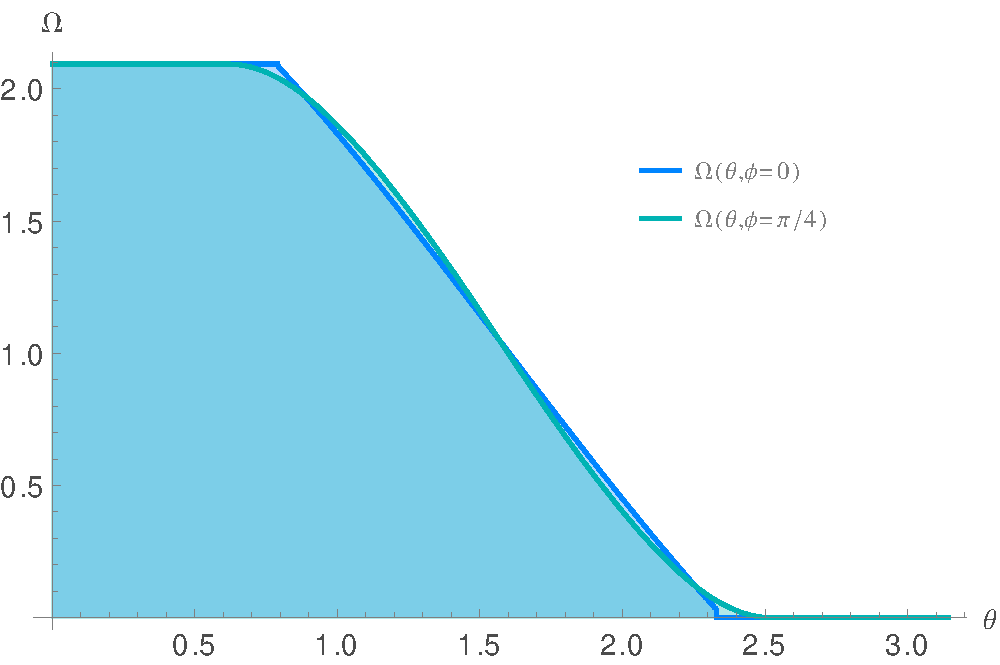
\includegraphics[width=0.4\textwidth]{\rootPath Imgs/graphs/on.pdf}
	\caption{Évolution de $\Omega_F(\vec n)$ selon l'orientation de $\vec n$}
	\label{fig:curve:omega_theta}
\end{figure}

Les poids affectés aux valeurs de chaque face de l'envmap sont donc l'intégration du produit scalaire normalisé $\frac{\vec\omega.\vec n}{\|\vec \omega\|}$ par rapport à l'angle solide sur la face considéré
\begin{align}
	W_F(\vec n)
		&= \iint_{F}\frac{\vec\omega.\vec n}{\|\vec \omega\|}\times\frac{\Hs(\vec\omega.\vec n)}{\|\vec\omega\|^3}\, \mathrm d\omega \notag\\
		&= \iint_{F}\frac{\vec\omega.\vec n\times\Hs(\vec\omega.\vec n)}{\|\vec\omega\|^4}\, \mathrm d\omega
		\label{ref:eq:wintegral}
\end{align}

\begin{figure}[!ht]
	\centering
	\includestandalone[width=0.4\textwidth]{\rootPath Figures/cubemapFacet}
	\caption{Intégration de l'envmap par rapport à une facette}
	\label{fig:tikz:envmapFacet}
\end{figure}

On notera qu'on a bien 
\begin{subequations}
	\begin{align}
					& \sum_{F \in Faces} \Omega(F) 								&=4\pi\\
	\forall \vec n	& \sum_{F \in Faces} \Omega(F,\vec n)	&=2\pi\\	
	\forall \vec n	& \sum_{F \in Faces} W_F(\vec n)			&=\pi	
	\end{align}
\end{subequations}

Dès lors, l'approximation selon laquelle $\mathcal L$ est constante sur chaque face nous donne
\begin{align}
	\mathcal E(p, \vec n)
		& = \frac{\mathcal P_{\mathcal V}(p)}{\pi}\sum_{F \in Faces}\mathcal L_{glob}(\vec F)W_F(\vec n) \notag \\
		& = \frac{\mathcal P_{\mathcal V}(p)}{\pi}\sum_{F \in Faces}\mathcal L_{glob}(\vec F)\iint_{F}\frac{\vec\omega.\vec n\times\Hs(\vec\omega.\vec n)}{\|\vec\omega\|^4}\, \mathrm d\omega
		\label{ref:eq:sumintegral_model}
\end{align}


\subsection{Approximation numérique}


En considérant la face $F_{Z^+}$ on obtient (sans perte de généralité)
\begin{multline}
	W_{F_{Z^+}}(\vec n) = \iint\limits_{[-1;1]^2} \biggl[\frac{(x.\vec n_x+y.\vec n_y + \vec n_z)}{(x^2+y^2+1)^2} \\
	\Hs(x.\vec n_x+y.\vec n_y + \vec n_z)\, \mathrm dx\, \mathrm dy\biggr]
\end{multline}

Le problème est alors de trouver un moyen de calculer, ou au moins d'approcher, la fonction $W_F(\vec n)$. Ce calcul étant par ailleurs fait  en chaque nœud du maillage, il est primordial de le faire en utilisant un minimum de ressource, quitte à évaluer une valeur approchée qui affectera le résultat de manière faible comparativement avec l'approximation faite précédemment et selon laquelle $\mathcal L$ est constante sur chacune faces.

\begin{figure}[!ht]\centering
	\begin{subfigure}[b]{0.4\textwidth}\centering
		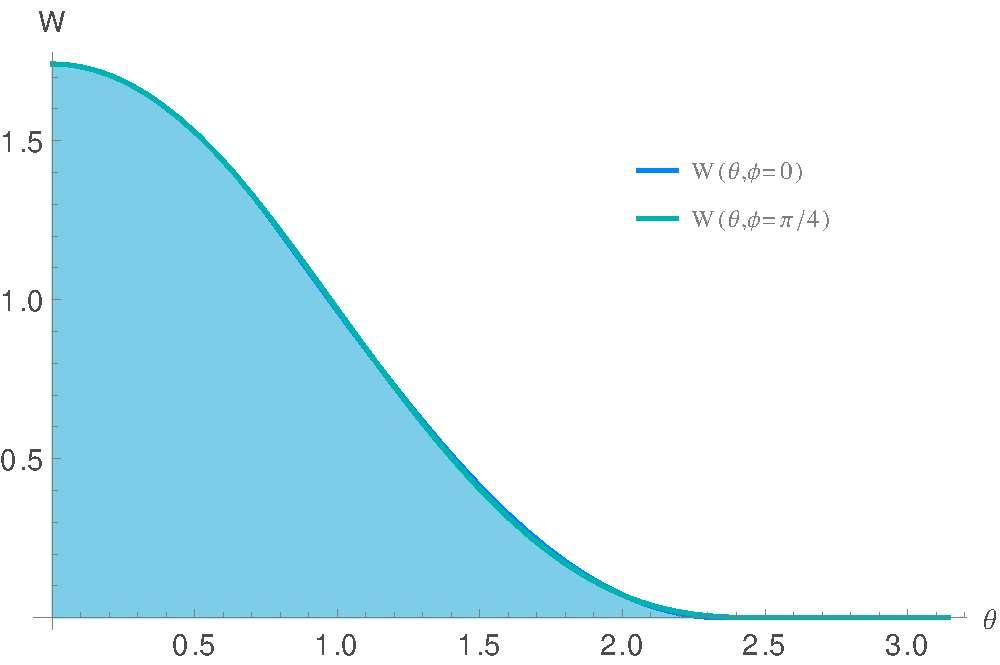
\includegraphics[width=\textwidth]{\rootPath Imgs/graphs/wn.pdf}
		\caption{$W(\theta)$}
	\end{subfigure}
	\begin{subfigure}[b]{0.4\textwidth}\centering
		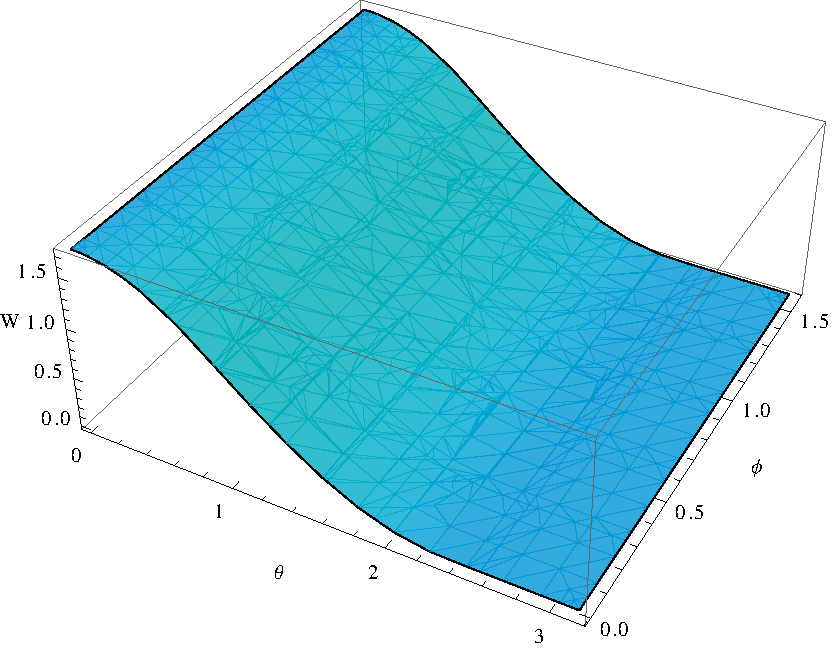
\includegraphics[width=\textwidth]{\rootPath Imgs/graphs/wn3D.pdf}
		\caption{$W(\theta,\phi)$}
	\end{subfigure}

	\caption{Évolution de $W_F(\vec n)$ selon l'orientation de $\vec n$ }
	\label{fig:curve:w_theta_phi}
\end{figure}

Comme le montre la figure~\ref{fig:curve:w_theta_phi}, la fonction $W_F$ dépendant principalement de $\theta$ on tentera de l'approximer par une fonction de $\vec n.\vec F = \cos(\theta)$

Une approximation simple est la fonction
\begin{equation}
	approx : \cos(\theta)\mapsto
	\frac{\bigl[\max\left(.75 + \cos(\theta), 0\right)\bigr]^2}{1.75}
\end{equation}
Comme le montre la figure \ref{fig:curve:w_approx}, cette fonction est, malgré sa grande simplicité proche de la fonction $W_F(\vec n)$.

\begin{figure}[!ht]\centering
	\begin{subfigure}[b]{0.4\textwidth}\centering
		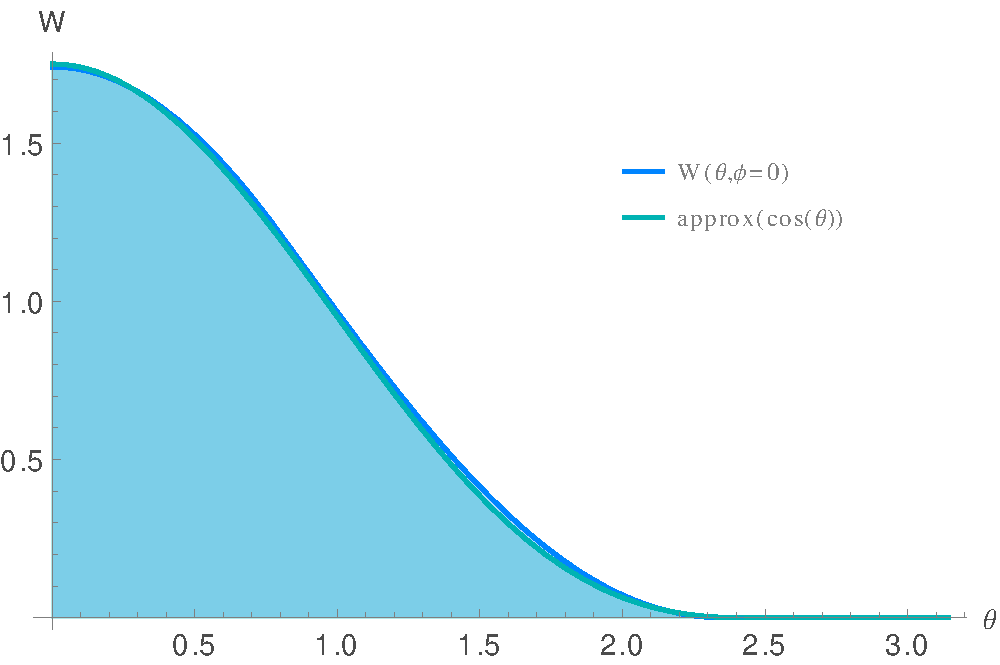
\includegraphics[width=\textwidth]{\rootPath Imgs/graphs/approxw.pdf}
		\caption{$W(\theta)$ et $approx(\cos(\theta))$}
	\end{subfigure}
	\begin{subfigure}[b]{0.4\textwidth}\centering
		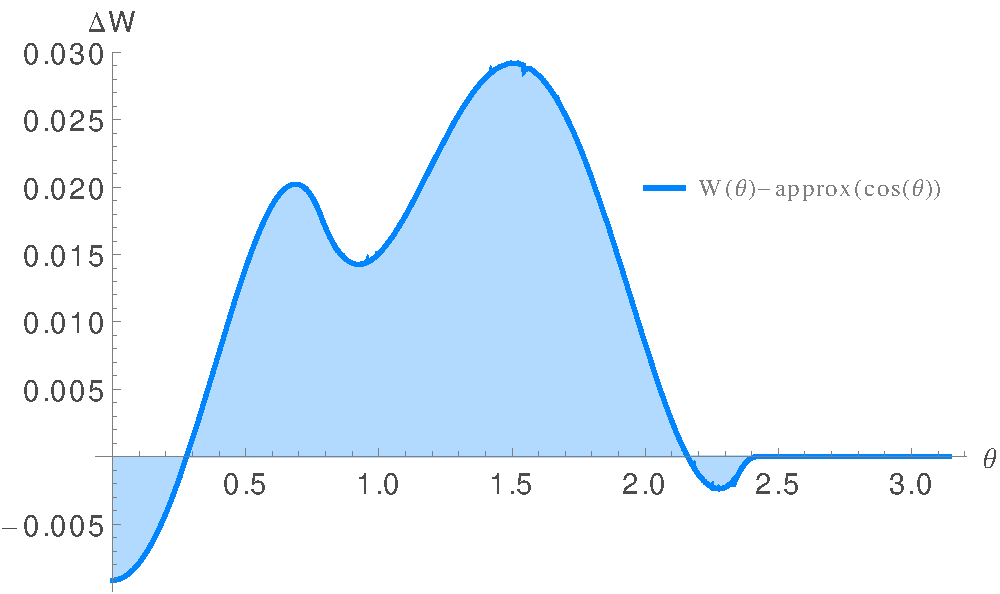
\includegraphics[width=\textwidth]{\rootPath Imgs/graphs/deltaw.pdf}
		\caption{$\Delta W$}
	\end{subfigure}
	\caption{Comparaison entre $W_F(\vec n)$ et $approx(\cos(\theta))$ }
	\label{fig:curve:w_approx}
\end{figure}


\subsection{Discussion}

La méthode développée ici repose sur l'approximation de la formule~(\ref{ref:eq:sumintegral_model}) et plus particulièrement de l'intégrale présenté dans la formule~(\ref{ref:eq:wintegral}). La complexité de cette intégrale réside dans le domaine effectif d'intégration, conditionné a la fois par la forme carré des faces de l'envmap et la présence d'un terme caractéristique de l'hémisphère visible.

Plusieurs formules ont été étudiée pour des domaines d'intégration hémisphériques ou partiellement hémisphérique ainsi que pour des polygones entièrement visibles \cite{Snyder1996} (ce qui fait disparaître le terme de $\Hs$).

Il aurait été possible d'adapter un modèle polygonale évoqué dans \cite{Snyder1996} mais les polygones sur lesquels il aurait fallu intégrer variant selon les conditions de visibilités il aurait été nécessaire d'effectuer de coûteux calculs de géométrie.

L'objectif principal étant ici une grande vitesse d'exécution, l'inexactitude des résultats étant de toute façon largement oubliée au regard des approximations faites précédemment on préféra utiliser une fonction grossièrement approché mais simple à calculer.


%%=====================================================================


\section{Ombrage}\label{section:ombres}

\subsection{Modèle}

Un indice visuel primordiale à la vraisemblance visuel des images produites est la présence d'ombres portées provoquées par l'ajout de l'objet \todo{reference}.

La modélisation de l'impact d'un tel ajout peut théoriquement être calculé qu'en connaissant la géométrie de la scène et la nature des matériaux qui la compose.

On fera ici plusieurs hypothèses dans le but d'obtenir un modèle qui soit calculable en temps réels tout en donnant des résultats vraisemblables.

Le calcul d'ombre douces est alors fait en décomposant l'objet en une hiérarchie de sphère comme présenté dans\cite{Iwanicki} et en sommant les contribution des différentes sphères.

Pour évaluer l'ombre douce projeté par une sphère il suffit alors d'évaluer le manque d'illumination.
On rappel les formules suivantes
\begin{align*}
	\mathcal E_{ambiant}(p, \vec n)	&=	\frac{1}{\pi}\int_{\mathcal{H}^2(\vec{n})}\mathcal L_{glob}(\vec\omega)\times\vec\omega.\vec n\, \mathrm d\vec\omega \\
	\mathcal E_{ombre}(p, \vec n)		&=	\mathcal E_{ambiant}(p, \vec n) - \frac{1}{\pi}\int_{\mathcal{S}(p)}\mathcal L_{glob}(\vec\omega)\times\vec\omega.\vec n\, \mathrm d\vec\omega
\end{align*}

avec $\mathcal S(p)$ la portion de sphère visible depuis la point considéré.

L'ombre est rendu en assombrissant le pixel associé ce point d'un facteur
\begin{align}
	\mathcal F(p)	&=	\frac{\mathcal E_{ombre}(p, \vec n)}{\mathcal E_{ambiant}(p, \vec n)}	\notag \\
								&=	1 - \frac{\int_{\mathcal{S}(p)}\mathcal L_{glob}(\vec\omega)\times\vec\omega.\vec n\, \mathrm d\vec\omega}{\int_{\mathcal{H}^2(\vec{n})}\mathcal L_{glob}(\vec\omega)\times\vec\omega.\vec n\, \mathrm d\vec\omega}	
\end{align}


Les différents niveaux de détail de l'envmap nous permettant d'obtenir des approximations de $L(p,\vec\omega)$ sur $\mathcal S(p)$ et sur $\mathcal{H}^2(\vec{n})$ on peut simplifier la formule en :

\begin{align}
	\mathcal F(p)	&=	1 - \frac{\mathcal L_{glob}(\mathcal{S}(p))}{\mathcal L_{glob}(\mathcal{H}^2(\vec{n}))}\left(\frac{1}{\pi}\int\limits_{\mathcal{S}(p)}\vec\omega.\vec n\, \mathrm d\vec\omega\right)
\end{align}

\begin{figure}[!ht]
	\centering
	\includestandalone[width=0.4\textwidth]{\rootPath Figures/shadows}
	\caption{Obstruction par une sphere}
	\label{fig:tikz:obstruction}
\end{figure}

Le calcul de l'angle solide formé par la sphère, et pondéré par un cosinus est détaillé dans \cite{Snyder1996}. On retiendra que dans notre cas ou la sphère est supposée au dessus du plan sur lequel se projettent les ombres :
\begin{equation}
	\int_{\mathcal{S}(p)}\vec\omega.\vec n\, \mathrm d\vec\omega = \cos(\omega)\sin^2(\alpha)
\end{equation}
avec $\alpha$ le demi angle sous lequel est vu la sphère et $\omega$ l'angle entre la vertical (normale à la surface sur laquelle se projettent les ombres) et la direction de la sphère.

On obtient ainsi :
\begin{align}
	\mathcal F(p)	&=	1 - \cos(\omega)\sin^2(\alpha)\frac{\mathcal L_{glob}(\mathcal{S}(p))}{\mathcal L_{glob}(\mathcal{H}^2(\vec{n}))}
\end{align}


\subsection{Discussion}

La ou il est habituel de segmenter l'environnement pour en extraire une hiérarchie de sources lumineuses, la méthode proposée ici permet d'évaluer des ombres douces à partir de données d'environnement sans étape de segmentation ni calcul de visibilité. 

Un développement intéressant serait de construire une décomposition hiérarchique, potentiellement intégrée dans un octree, et de l'évaluer plus ou moins profondément selon la distance considérée.


%=====================================================================

\section{Reflets spéculaires}

Le calcul de l'éclairage ambiant revient à considérer une BRDF purement lambertienne. Afin d'améliorer le réalisme du rendu il convient d'adopter un modèle de Phong en ajoutant une part d'éclairage spéculaire.

Cet éclairage spéculaire permet de rendre de manière intéressante des surfaces métallique, dans la limite d'un seul reflet. Le modèle adopté ici est par ailleurs isotrope, ce qui ne permet par le rendu de matières comme du métal brossé pour lesquels on retrouve des directions privilégiés.

Dans notre cas l'évaluation du reflet se fait naturellement en calculant la réflexion du rayon incident, donné par la position du point considéré dans l'espace de la camera, relativement à la normale de l'objet dans ce même espace. On accédera ensuite à la valeur d'éclairage directement dans l'envmap.

Une fois de plus on pourra utiliser les différents niveaux de mipmap à notre avantage, la considération du niveau de mipmap revenant la considérer l'angle d'un cône autour de l'axe du reflet. Un tel cône permet ainsi de caractériser le caractère spéculaire de l'objet, cette dernière pouvant varier d'un reflet parfait --miroir-- à un reflet plus diffus --plastique--.
On utilisera également l'ombre projeté calculé précédemment afin de moduler les reflets.

%=====================================================================

\section{Vers un modèles à micro-facettes}

Les modèles employés ici permettent un rendu rapide mais présentes des limitations en terme de qualité. Il serait intéressant, dans l'optique améliorer encore la qualité du rendu, de considérer un modèle à micro-facette. 
Le principes des modèles à micro-facette est de considérer la surface de l'objet comme un ensemble de petites faces orientés selon des normales propres a chacune (micro-normales). La distribution statistique des micro-normales autour de la normale géométrique du maillage (macro-normale) permet de déterminer les mécanismes de réflexion. Parmi les nombreux avantages d'un telle méthode il y a la possibilité de caractériser des surfaces anisotropes par le biais de directions privilégiés dans la distribution de facettes.

L'auto-occultation entre facettes, variable selon le point de vue, permet par ailleurs de calculer une normal intermédiaire entre la normale géométrique et les micro-normales des facette (mézo-normal) qui correspond à l’intégration des micro-normales sur l'ensemble des facette visible\cite{Bruneton2010}\cite{Heitz2013} \todo{figure}. Cette mézo-normale, utilisée à la place de normale géométrique, permet de corriger les reflets sur des surfaces vue sous un angle important.

L’intégration complète d'un tel modèle à été envisagé de la manière suivante :
\begin{enumerate}
	\item Choix d'une distribution de normale (gaussienne) et étude du modèle associé;
	\item Ajout aux objets 3D d'une texture (optionnelle) caractérisant localement la direction privilégiée et la force de l'anisotropie associée;
	\item Évaluer, dans le fragment shader, la distribution de direction reflétées en fonction de l'angle de vue et des caractéristiques stockées dans la texture;
	\item Évaluer la lumière incidente selon la distribution calculée précédemment.
\end{enumerate}

Au delà des calcul complexes, mais heureusement déjà documentées, du premier point\cite{Heitz2013a}, l'évaluation de l'envmap selon des distributions anisotrope nécessite de lourds calculs.
Il serait possible de les réduire fortement via un pré-calcule (convolution) mais dans notre cas le caractère dynamique de l'environnement ne permet pas un telle approche.

Dans notre cas, il serait nécessaire d'évaluer, sans pré-calcul, l’intégration anisotrope de l'envmap.
Les outils de filtrages anisotropes ne sont ici pas exploitable en l’état car une filtre anisotrope est définit entre autre par le facteur d'anisotropie qui le caractérise. Le nombre d'unité de texture étant grandement limité, il n'est pas possible de charger plusieurs fois l'envmap avec des filtrages différents qui couvriraient toutes nos attentes.

Les outils de lecture de texture par gradient\footnote{\href{https://www.opengl.org/sdk/docs/man/html/textureGrad.xhtml}{\texttt{textureGrad()}}} mis en place dans openGL ne conviennent pas non plus car même si les vecteurs fournis (\texttt{dX} et \texttt{dY}) sont caractéristique d'une forte anisotropie, seul celui de norme maximal compte dans l'évaluation de l’accès au niveau de texture. 

Il conviendrait donc, pour permettre en place les mécanismes d'évaluation anisotrope voulus, d'approximer l’intégration vis de multiples accès à la texture, le long de la direction privilégie d’anisotropie pour procéder à une intégration implicite.

%=====================================================================

\section{Pipeline}

\begin{figure*}
	\centering
	\includestandalone[width=0.8\textwidth]{\rootPath Figures/pipeline}
	\caption{Pipeline développé}
	\label{fig:tikz:pipeline}
\end{figure*}

Compte tenu des méthodes décrites précédemment, le pipeline de rendu se décompose en différentes parties (voir figure~\ref{fig:tikz:pipeline})
\begin{enumerate}
	\item L'étape de pré-calcul permet l'évaluation de données propres au modèle. Ces données n'étant pas influencé par la localisation dans l'espace ni par les caractéristiques d'environnement lumineux, il n'est pas nécessaire de les recalculer en temps réelle et on préféra donc stocker les résultats pré-calculés.
		\begin{description}
			\item[Ambiant :] information d'auto-occultation ($\mathcal P_{\mathcal V}(p)$), stocké dans une \texttt{texture2D};
			\item[Sphères :] décomposition de l'objet comme union de sphères, stocké sous forme de \texttt{vec4[]}.
		\end{description}

	\item L'étape de calcul temps réel, qui évalue des résultats temporaires nécessaires à la réalisation du rendu final. Ces résultats doivent êtres réévaluer dynamiquement car ils dépendent de paramètres dynamique tel que les données d'environnement.
		\begin{description}
			\item[Ombre :] ombre douce projeté par l'objet, elle dépend de l'environnement lumineux décrit par l'envmap.
		\end{description}
	
	\item L'étape de rendu qui produit l'image telle qu'elle est vue par l'utilisateur.
		\begin{description}
			\item[Rendu objet :] affichage de l'objet, en tenant compte de l'éclairage ambiant, et des reflets spéculaires;
			\item[Rendu ombre :] affichage des ombres en surimpression afin d'intégrer l'objet ne manière plus réaliste.
		\end{description}
\end{enumerate}

%=====================================================================

\section{Résultats}







%=====================================================================
%=====================================================================
\ifstandalone
	\addcontentsline{toc}{chapter}{Bibliographie}
	\bibliographystyle{apalike}
	\bibliography{\rootPath Annexes/biblio}
\fi
%=====================================================================
%=====================================================================

\end{document}
\documentclass[10pt,a4paper,twoside, twocolumn]{report}
%% Lots of packages !
\usepackage{etex}

%% Francisation
\usepackage[francais]{babel}
\usepackage[T1]{fontenc}
\usepackage[utf8]{inputenc}
%\usepackage{textcomp}

%% Réglages généraux
\usepackage[left=1.5cm,right=1.5cm,top=2cm,bottom=2cm]{geometry}
\usepackage{fancyhdr}
\usepackage{setspace}
\usepackage{lscape}
%\usepackage{multicol}
\usepackage{makeidx}
\usepackage[clearempty]{titlesec}
\usepackage{cite}

%% Packages pour le texte
\usepackage{pifont}
\usepackage{eurosym}
\usepackage{soul}
\usepackage[normalem]{ulem}
\usepackage{fancybox}
\usepackage{boxedminipage}
\usepackage{enumerate}
\usepackage{verbatim}
\usepackage{moreverb}
\usepackage{listings}
\usepackage[table]{xcolor}

%% Packages pour les tableaux
\usepackage{array}
\usepackage{multirow}
\usepackage{tabularx}
\usepackage{longtable}

%% Packages pour les dessins
\usepackage{graphicx}
\usepackage{wrapfig}
%\usepackage{picins}
\usepackage{picinpar}
\usepackage{epic}
\usepackage{eepic}
\usepackage{tikz}
\usepackage{afterpage}
\usepackage{rotating}
\usepackage{float}
\usepackage{caption}

%% Packages pour les maths
\usepackage{amsmath}
\usepackage{amssymb}
\usepackage{dsfont}
\usepackage{mathrsfs}
\usepackage{bussproofs}
\usepackage[thmmarks,amsmath]{ntheorem}

%% Création de nouvelles commandes
%\usepackage{calc}
\usepackage{ifthen}
\usepackage{xspace}



\usepackage{url}
\usepackage{hyperref}
\usepackage{todonotes}
\usepackage{subcaption}
\usepackage[french,ruled,vlined,linesnumbered,algochapter,dotocloa]{algorithm2e}
\usepackage{MnSymbol}

\usepackage{chngcntr}

\usepackage{standalone}
\usepackage{import}



\frenchbsetup{StandardEnumerateEnv=true}

%% =======================================================================

\fancypagestyle{empty}{%
  \fancyhf{}
  \fancyhead[L]{}
  \fancyhead[C]{}
  \fancyhead[R]{}
  \fancyfoot[L]{}
  \fancyfoot[C]{}
  \fancyfoot[R]{}
}
\fancypagestyle{basicstyle}{
	\fancyhf{}	
	\fancyhead[L]{}
	\fancyhead[C]{Rendu réaliste et temps réel pour la réalité augmentée}
	\fancyhead[R]{}
	\fancyfoot[L]{hadrien.croubois@ens-lyon.fr}
	\fancyfoot[C]{--~\thepage~--}
	\fancyfoot[R]{}
}
\pagestyle{basicstyle}

%% =======================================================================

\titleformat{\section}[frame]
{\normalfont}
{\filright \footnotesize \enspace Partie \thesection\enspace}
{6pt}
{\bfseries\filcenter}
	
\titleformat{\subsection}[frame]
{\normalfont}
{\filright \footnotesize \enspace \thesubsection\enspace}
{6pt}
{\filcenter}

\titleformat{\subsubsection}
{\titlerule \vspace{.8ex} \normalfont\itshape}
{\thesubsubsection}
{.5em}
{}

\titleformat{\chapter}[display]
{\normalfont\bfseries\filcenter}
{}
{1ex}
{\titlerule[2pt] \vspace{2ex} \LARGE}
[\vspace{1ex} {\titlerule[2pt]}]

\parindent=10pt
\DeclareUnicodeCharacter{00A0}{~}

%% =======================================================================



\newcommand{\HRule}{\rule{\linewidth}{0.5mm}}
\newcommand{\Hs}{\operatorname{HS}}




\floatstyle{ruled}
\restylefloat{figure}
\restylefloat{table}
\newfloat{code}{!h}{locode}{}
\floatname{code}{\textsc{code}}

\addto\captionsfrench{%
  \renewcommand{\listfigurename}{Liste des figures}%
  \renewcommand{\listtablename}{Liste des tableaux}%
  \renewcommand{\listalgorithmcfname}{Liste des algorithmes}%
}
\newcommand{\listofcode}{\listof{code}{Liste des codes}}

\numberwithin{code}{chapter}
\numberwithin{equation}{subsection}
\counterwithout{footnote}{chapter}






\newcommand{\framedgraphics}[2]{%
  \setlength{\fboxsep}{0pt}%
  \setlength{\fboxrule}{1pt}%
  \fbox{\includegraphics[{#1}]{{#2}}}%
}

\newcommand*{\captionsource}[2]{%
  \caption[{#1}]{%
    #1%
    \\\hspace{\linewidth}%
    \textbf{\textsc{Source}} #2%
  }%
}

\newcommand{\footurl}[2][]{\footnote{\textbf{#1}\href{#2}{#2}}}
% \newcommand{\footurl}[2][]{\footnote{\textbf{#1}\url{#2}}}







\newif\iftwocolumn
\twocolumntrue
\usetikzlibrary{3d,arrows, calc, backgrounds, petri, positioning, shadows, shapes}


\tikzset{
	persp/.style={scale=3.0,x={(-0.8cm,-0.4cm)},y={(0.8cm,-0.4cm)}, z={(0cm,1cm)}},
	points/.style={fill=white,draw=black,thick}
	grid/.style={very thin,gray},
	axis/.style={->,ultra thick},
	cube/.style={thick, fill=black!15,opacity=0.5},
	cube hidden/.style={dashed},
	block/.style={
		rectangle, rounded corners,
		draw=black!80,
		fill=black!10, fill opacity=0.5,
		text=black!90, text opacity=1.0,
    text height=1.5ex,
    text depth=.25ex,
    text width=6em,
    text centered
	}
}

\tikzstyle{class}			=[rectangle, rounded corners, draw=black, fill=blue!40, drop shadow, text centered, anchor=north, text=white,    text width=3cm]
\tikzstyle{module}		=[rectangle, rounded corners, draw=black, fill=red!40, 	drop shadow, text centered, anchor=north, text=white,    text width=3cm]
\tikzstyle{component}	=[rectangle, rounded corners, draw=black, fill=green,   drop shadow, text centered, anchor=north, text=black!90, text width=3cm]
\tikzstyle{single}		=[text height=1.5ex, text depth=0.25ex]
\tikzstyle{double}		=[text height=4.0ex, text depth=2.75ex]
\tikzstyle{triple}		=[text height=6.5ex, text depth=5.25ex]
\tikzstyle{quadru}		=[text height=9.0ex, text depth=7.75ex]
\newcommand*{\rootPath}{../}
\standalonetrue

\begin{document}


\iftwocolumn \twocolumn \else \onecolumn \fi


\chapter{Pré-calculs}

Nous avons détaillé dans le chapitre précédent les différentes étapes de rendu pour l'intégration d'un objet 3D dans une scène dynamique acquise en temps réel. Certaines des données nécessaires à un tel rendu étant indépendantes de la scène, nous nous sommes proposés de les pré-calculer. 

\section{Éclairage ambiant sous forme de texture}\label{section:precomputation_ambiant}

Nous avons vu dans la section~\ref{section:ambiant}, page~\pageref{section:ambiant}, le calcul de l'éclairage ambiant. Dans ce calcul intervenait un terme d'auto-occultation propre à l'objet 3D considéré.
\begin{align}
	\mathcal P_{\mathcal V}(p) = \frac{1}{\pi}\int_{\mathcal V(p, \vec n(p))}\vec\omega.\vec n\, \mathrm d\vec\omega
\end{align}

\subsection{Intégration statistique}
Il s’agit donc d'évaluer, en tout point de l'objet, l’intégrale du produit scalaire entre le vecteur d’intégration et la normale à l'objet, pour un vecteur d’intégration parcourant l’espace visible.

On peut alors reformuler le calcul comme suit :
\begin{align}
\mathcal P_{\mathcal V}(p)	&= \frac{1}{\pi}\int_{\mathcal V(p, \vec n(p))}\vec\omega.\vec n\, \mathrm d\vec\omega \notag\\
														&= \frac{1}{\pi}\int_{\mathcal H^2(\vec n(p))}\vec\omega.\vec n\times visible(p, \vec \omega)\, \mathrm d\vec\omega \notag\\
														&= \frac{1}{\pi}\int_{\mathcal S}\vec\omega.\vec n\times \Hs(\vec \omega.\vec n)\times visible(p, \vec n)\, \mathrm d\vec\omega
\end{align}

Pour évaluer une telle intégrale, on procède par une intégration statistique (Monte Carlo). Pour cela on simule le domaine d'intégration sur l'espace de définition en tirant $n$ points uniformément sur une sphère. Ces points représentent les vecteurs $\vec\omega$.

Pour chacun de ces points il s’agit d'évaluer :
	$$\vec\omega.\vec n\times \Hs(\vec \omega.\vec n)\times visible(p, \vec n)$$
Le terme $\Hs(\vec \omega.\vec n)$ est en fait inutile car tout point pour lequel $visible(p, \vec n)$ sera non nul sera assuré d’être dans l’hémisphère décrit par $\Hs(\vec \omega.\vec n)$. La fonction à intégrer peut donc se résumer à :
	$$\vec\omega.\vec n\times visible(p, \vec n)$$

\subsection{Évaluation de la visibilité}
L'évaluation la visibilité est faite à l'aide d'une shadowmap. Étant donné un point de vue (vecteur $\vec\omega$ aléatoire), il s’agit d’effectuer une première étape de rendu qui donnera, dans le Z-buffer, les informations de visibilité (voir figure~\ref{fig:precompute_ambiant:zbuffer}).

\begin{figure}[!ht]\centering
	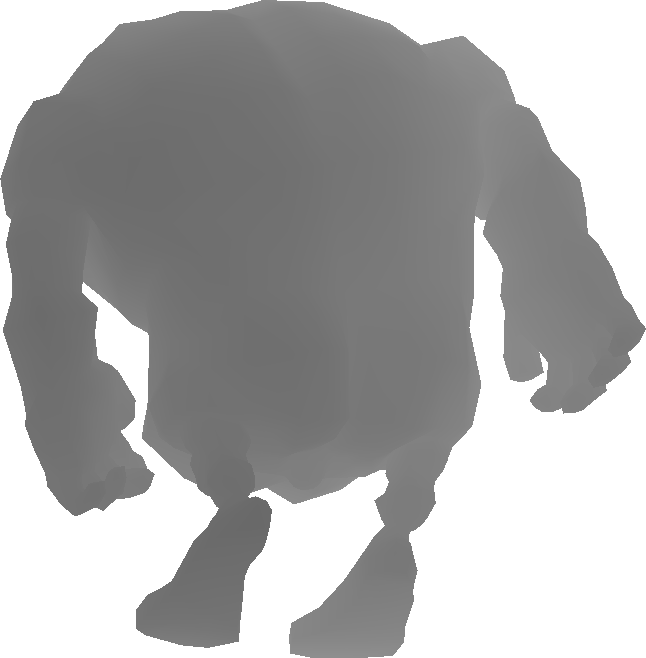
\includegraphics[width=0.4\textwidth]{\rootPath Imgs/precompute_ambiant/zbuffer.png}
	\caption{Z-buffer issu de la première étape de rendu (shadowmap)}
	\label{fig:precompute_ambiant:zbuffer}
\end{figure}


Ces données de profondeur permettent ensuite d'évaluer si un texel est visible ou non, simplement en comparant la profondeur du texel considéré et celui retenu dans la texture et qui caractérise le texel le plus proche selon le rayon associé.

La seconde étape de rendu consiste alors à écrire, dans l’espace texture associé à l'objet, les informations de visibilités qui auront été calculées (voir figure~\ref{fig:precompute_ambiant:singlesource}). À cette étape, il est important de s'assurer que la texture est bien écrite, y compris au niveau des jointures entre les différents éléments qui peuvent demander un ajustement.\cite{Aila2005}\cite{Manson2012}

\begin{figure}[!ht]\centering
	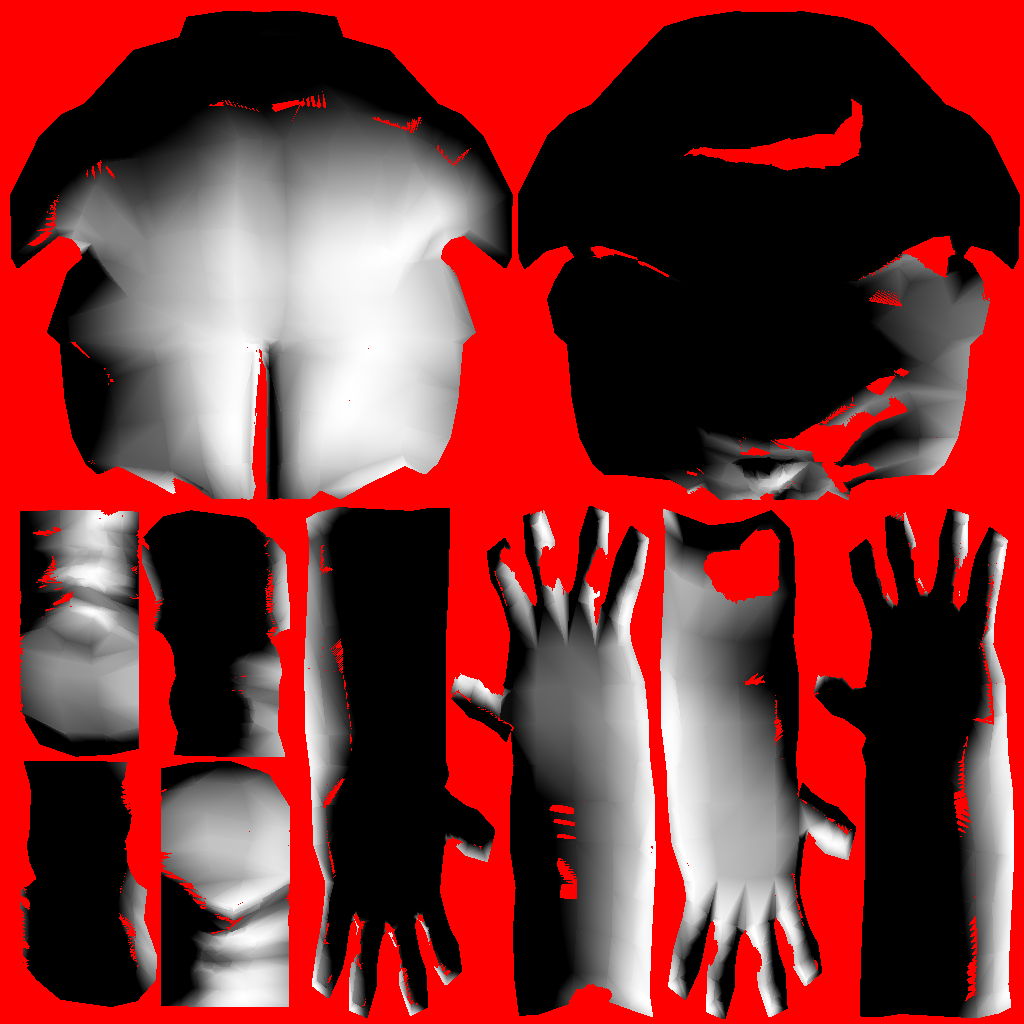
\includegraphics[width=0.4\textwidth]{\rootPath Imgs/precompute_ambiant/singlesource_red.png}
	\caption{Rendu en espace texture pour une source}
	\label{fig:precompute_ambiant:singlesource}
\end{figure}

\subsection{Post-traitement}
Une fois évalués pour une source, les résultats sont ajoutés à une texture qui somme les contributions des différentes sources. Cette texture contient ainsi le résultat de l'intégration considérée.

Une fois toutes les sources évaluées, il reste quelques étapes de post-traitement :
\begin{itemize}
	\item L'intégration étant normalisée, les valeurs calculées sont théoriquement entre $0.0$ et $1.0$. Cependant du fait de la distribution aléatoire des sources utilisées pour l'intégration, il peut arriver qu'en certains points ne pressentant pas d'auto-occultation la valeur dépasse $1.0$. Les valeurs sont alors seuillées afin de ne pas poser de problèmes au moment du stockage au format \texttt{.png}.

	Les données étant quantifiées entre $0$ et $255$, un dépassement de la valeur flottante à stocker peut provoquer une traduction en un entier supérieur à $255$. Ces nombres étant stockés sous forme de caractères ASCII, un dépassement à $256$ ou $257$ peut alors provoquer une évaluation modulo $256$ soit un stockage sous forme de $0$ ou de $1$.

	\item Les parties de l'image ne correspondant pas à des coordonnées de textures valides étant jusque-là vides. L'évaluation des niveaux de mipmap pour la texture considérée risque de prendre en compte des éléments qui ne sont par représentatifs de la réalité géométrique de l'objet. Afin de limiter ce biais dans l'évaluation des niveaux de mipmap, on remplit les parties vides et non représentative avec la valeur moyenne calculée sur les parties représentatives. Ainsi on limite l’incohérence des données considérées en bordure de patch pour les niveaux de mipmap les plus élevés.
\end{itemize}

A l'issue de ces différents post-traitement, il ne reste qu'à exporter la texture sous forme d'image (voir figure~\ref{fig:precompute_ambiant:postprocess}) qui sera chargée le moment voulu.

\begin{figure}[!ht]\centering
	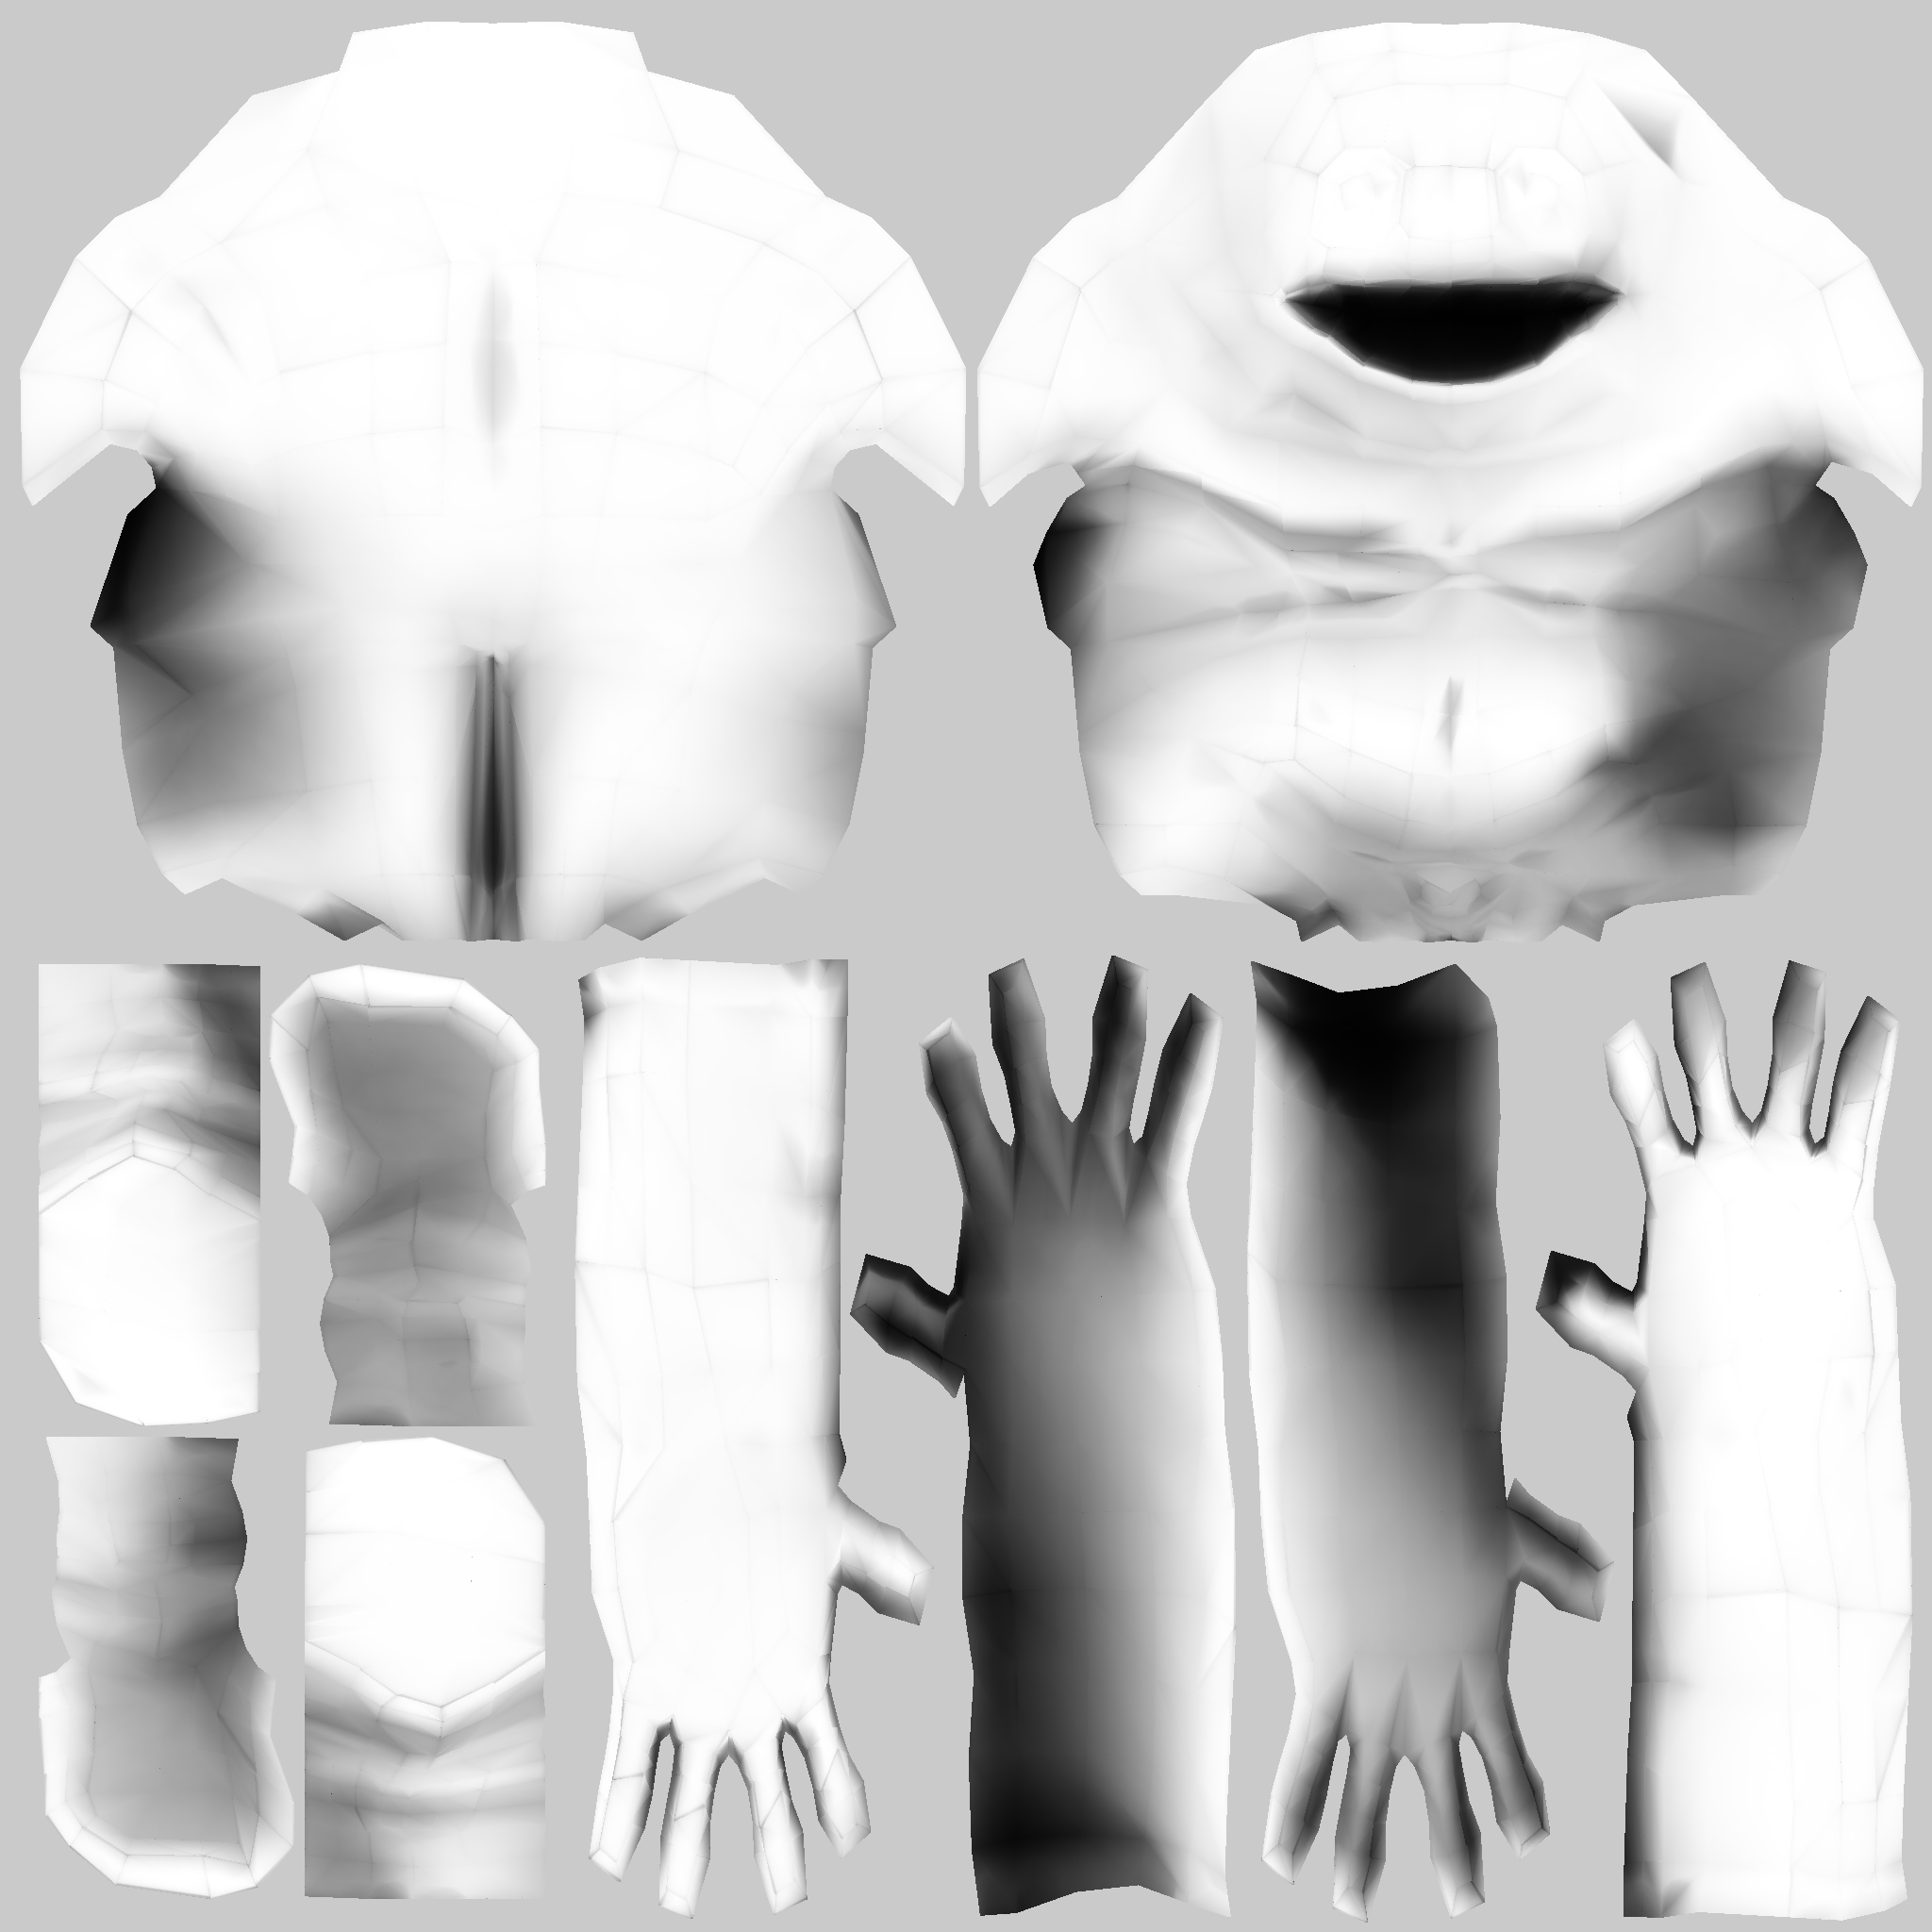
\includegraphics[width=0.4\textwidth]{\rootPath Imgs/precompute_ambiant/postprocess.png}
	\caption{Données pré-calculées en espace texture après post-traitement (1000 sources)}
	\label{fig:precompute_ambiant:postprocess}
\end{figure}

\begin{figure}[!ht]\centering
	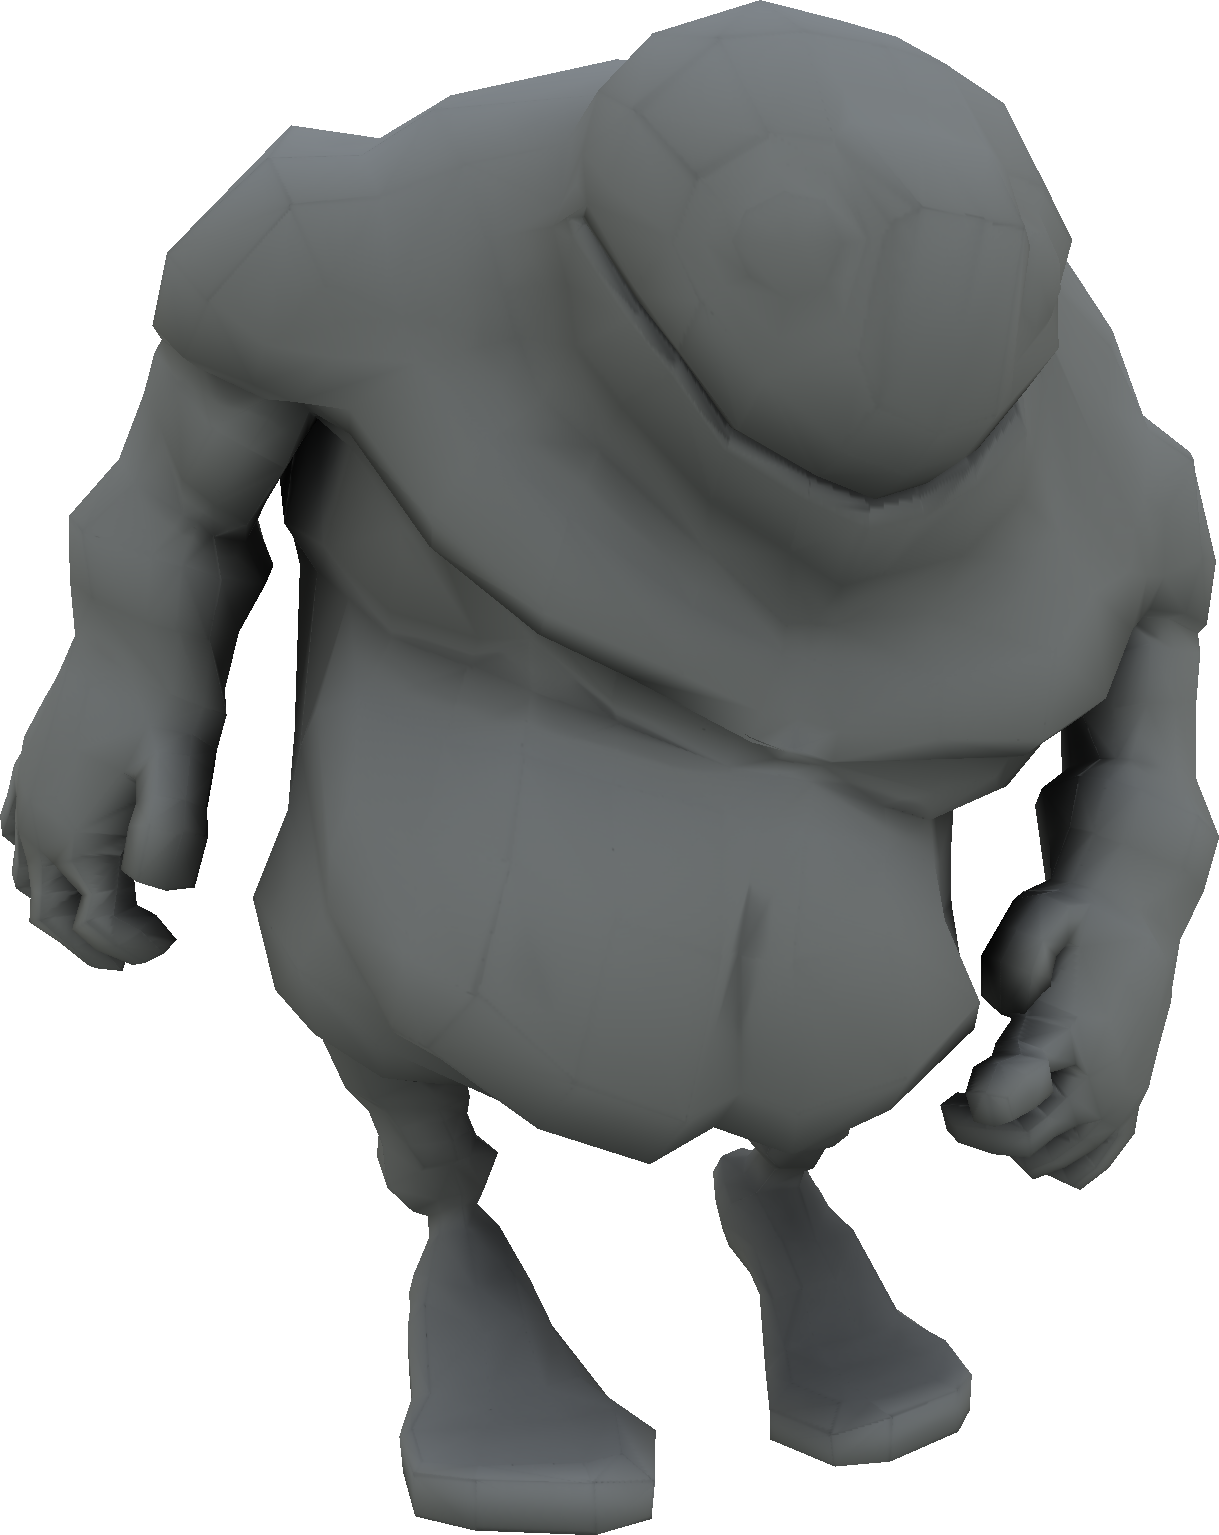
\includegraphics[height=4cm]{\rootPath Imgs/precompute_ambiant/view3.png}
	\hspace{0.5cm}
	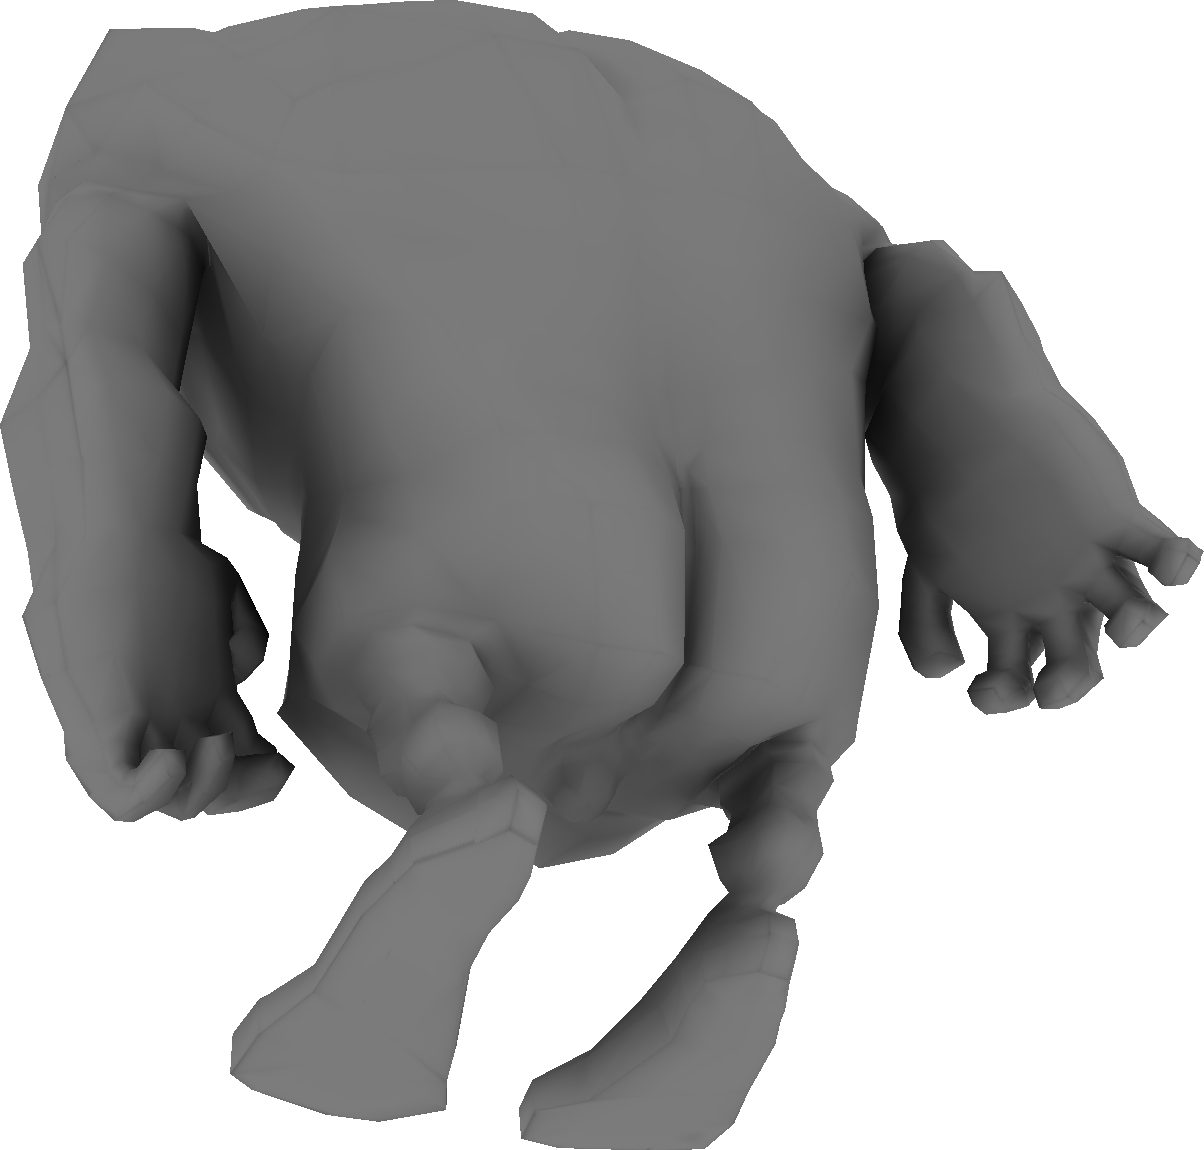
\includegraphics[height=4cm]{\rootPath Imgs/precompute_ambiant/view2.png}
	\caption{Utilisation des données d'éclairage ambiant lors du rendu}
	\label{fig:precompute_ambiant:view}
\end{figure}



\section{Décomposition en sphères}\label{section:precomputation_spheres}
La section~\ref{section:ombres}, page~\pageref{section:ombres}, traite du rendu d'ombres portées issues de l'objet 3D ajouté à la scène. Cette étape nécessite une représentation de l'objet en question comme union de sphères.

Le pré-calcul étudié ici consiste donc à construire, étant donné un maillage, un ensemble limites de sphères qui s'approche au mieux de la surface correspondant au maillage.

Ce problème d'optimisation est longuement développé dans la littérature\cite{Marshall1997}\cite{Gross2003}, notamment pour la reconstruction de surfaces implicites à partir de points (orientées ou non). La plupart des méthodes consistent à ajuster des surfaces contraintes à l'aide d'outils statistiques. Ces méthodes présentent cependant le défaut d’être mathématiquement complexes et numériquement complexes.

Le choix s'est donc porté sur une méthode simple et inexacte mais suffisante au regard de l'utilisation des résultats par l'algorithme de calcul des ombrages.

\begin{algorithm}[ht]
	\SetKwData{Mesh}{Maillage}
	\SetKwData{Point}{Point}
	\SetKwData{Sphere}{Sphere}
	\SetKwData{int}{int}
	\SetKwFunction{UniformSample}{EchantionnageUniforme}
	\SetKwFunction{Clustering}{Appareillement}
	\SetKwFunction{BestMatchingSphere}{SphereOptimale}

	\Entree{\Mesh $m$, \int $n$, \int $s$}
	\BlankLine
	\tcc{Échantillonnage du maillage}
	\Point $pts[s]$\;
	\Pour{$i \leftarrow [1..s]$}{
		$pts[i] \leftarrow \UniformSample(m)$\;
	}
	\BlankLine
	\tcc{Initialisation des sphères}
	\Pour{$i \leftarrow [1..n]$}{
		$sphs[i] \leftarrow pts[i]$\;
	}
	\BlankLine
	\Tq{$sphs$ n'est pas stable}{
		\Point $clsts[n][]$\;
		\Pour{$i \leftarrow [1..n]$}{
			$clsts[i] \leftarrow \Clustering(pts, sphs[i])$\;
		}
		\Pour{$i \leftarrow [1..n]$}{
			$sphs[i] \leftarrow \BestMatchingSphere(clsts[i])$\;
		}
	}
	\Retour{$sphs$}\;
	\caption{Ajustement de sphères à un maillage}
\end{algorithm}

\subsection{Échantillonnage du maillage}

Afin d'obtenir une distribution uniforme de points à la surface de l'objet, on procède à un échantillonnage par importance\footnote{Importance sampling}.

Pour construire un point uniformément à la surface du maillage, on sélectionne d'abord une face proportionnellement à sa surface avant de choisir un point uniformément sur la face considéré.

En répétant cette opération un grand nombre de fois on obtient un nuage de points qui représente correctement les grandes faces. Ce sont ces points qui seront utilisés par la suite pour la construction des sphères représentatives.

\subsection{Appareillement de points et calcul de sphères optimales}

La phase d'appareillement de l'algorithme consiste à organiser les points en clusters relatifs aux sphères déjà construites. Il s’agit donc d’établir une métrique qui caractérise la proximité d'un point à une sphère. De la même manière, la phase de calcul de sphères optimales consiste à calculer la sphère qui minimisera la métrique considère précédemment sur le cluster qui lui a été associé.

La principale difficulté ici est de construire un métrique représentative des critères de qualités voulus, pour laquelle le calcul d'un élément optimal n'est pas trop complexe et qui converge vers un état stable.

\subsubsection{Première approche}

Une métrique envisagéz est d'évaluer la distance d'un point à la surface de la sphère associé :
\begin{align}
	f(P, S) &= \left\|P-S\right\|^2 - S.r^2															\label{eq:metrique}	\\
					&= (P.x-S.x)^2 + (P.y-S.y)^2 + (P.z-S.z)^2 - S.r^2					\notag \\
					&= (P.x^2 + P.y^2+P.z^2) + (S.x^2+S.y^2+S.z^2)							\notag \\
					&\quad - 2(P.xS.x + P.yS.y + P.zS.z)  - S.r^2								\notag \\
					&= \|P\|^2 + \|S\|^2 - 2(P.xS.x + P.yS.y + P.zS.z) - S.r^2	\notag
\end{align}

Ce calcul de la sphère optimal associé a un cluster peut ensuite se faire par l'optimisation d'un système matriciel $AX-B$, la matrice $A$ représentant les données en entrée (points échantillonnées), le vecteur $X$ représentant la solution à optimiser et le vecteur $B$ étant l'objectif à atteindre.

L'équation~\ref{eq:metrique} nous indique comment construire $A$, $X$ et $B$ :
\begin{subequations}
\begin{align}
		A	&=	\begin{pmatrix}
						-2P_1.x & -2P_1.y & -2P_1.z & 1 			\\
						-2P_2.x & -2P_2.y & -2P_2.z & 1 			\\
						\vdots	& \vdots	&	\vdots	& \vdots	\\
						-2P_n.x & -2P_n.y & -2P_n.z & 1
					\end{pmatrix}																												\\
		X &=	\begin{pmatrix} S.x \\ S.y \\ S.z \\ \|S\|^2 - S.r^2 \end{pmatrix}	\\
		B	&=	\begin{pmatrix}
						\|P_1\|^2	\\
						\|P_2\|^2	\\
						\vdots			\\
						\|P_n\|^2
					\end{pmatrix}																												\\
\intertext{Ainsi on a :}
	A.X+B &= \begin{pmatrix}
						f(P_1, S)	\\
						f(P_2, S)	\\
						\vdots		\\
						f(P_n, S)
					\end{pmatrix}
\end{align}
\end{subequations}

Cette première considération géométrique n'est cependant pas satisfaisante. La simple proximité entre un point et la surface d'une sphère ne prend pas en compte les différences d'orientation de normale entre une face du maillage et la sphère qui le modélise, lesquels sont des éléments de qualité essentiels dans notre cas. Au delà de ce problème d'orientation, cette métrique fait aussi face au problème des outliers présents sur les modèles non convexes. Si quatre points extrémaux se retrouvent loin de tout, il est possible qu'une sphère viennent les adopter comme point d'attache, englobant alors tout le modèle et cachant la géométrie que l'on voulais représenter.

Par ailleurs la métrique proposé précédemment ne garanti pas la convergence du système.

\begin{figure*}[!ht]\centering
	\begin{subfigure}[b]{\textwidth}\centering
		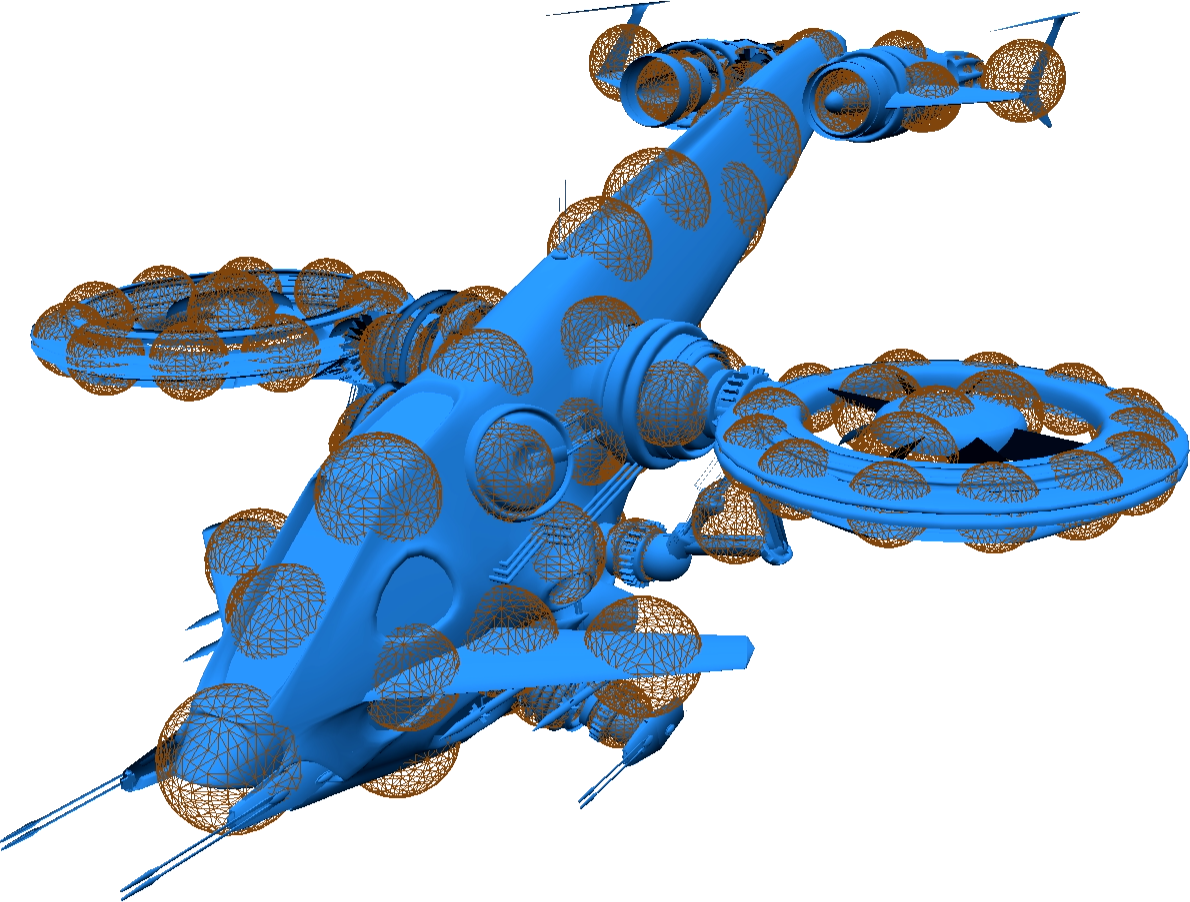
\includegraphics[width=0.4\textwidth]{\rootPath Imgs/precompute_spheres/MRX22_both.png}
		\vspace{0.5cm}
		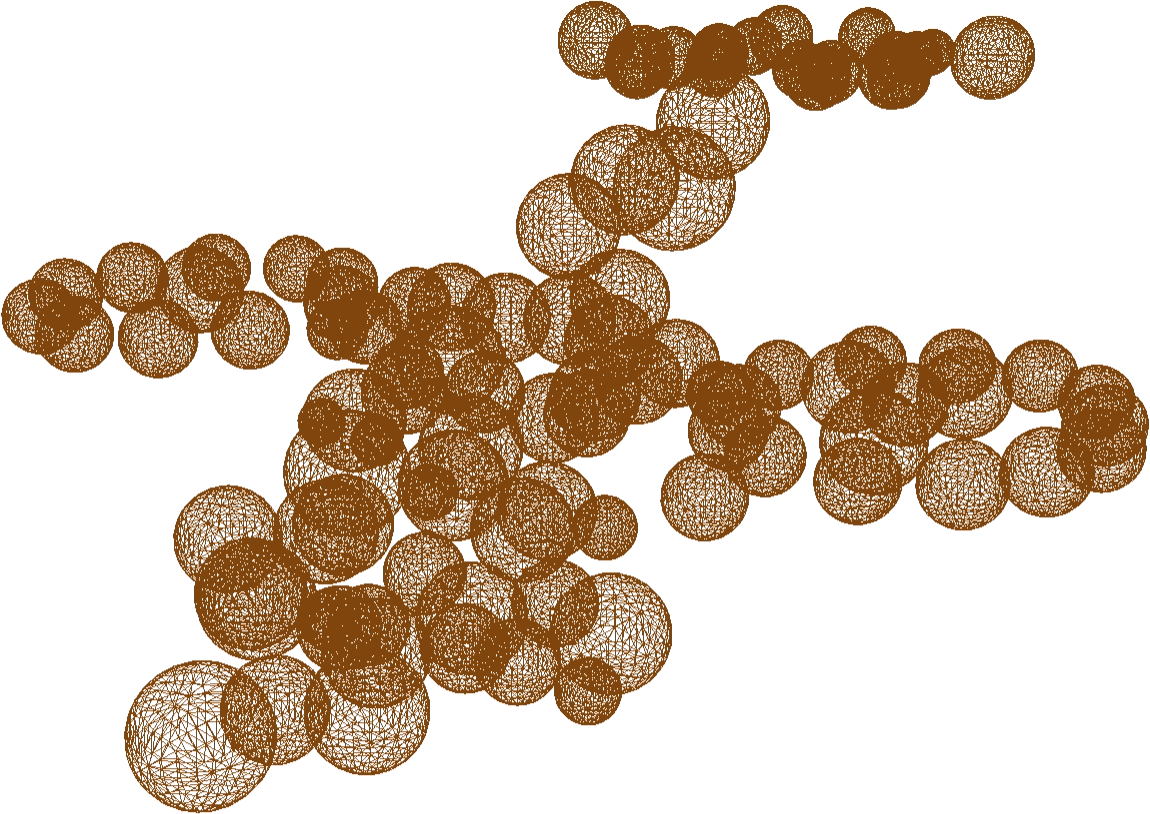
\includegraphics[width=0.4\textwidth]{\rootPath Imgs/precompute_spheres/MRX22_spheres.png}
		\caption{MRX22 (157781 sommets, 287776 triangles)}
	\end{subfigure}

	\begin{subfigure}[b]{\textwidth}\centering
		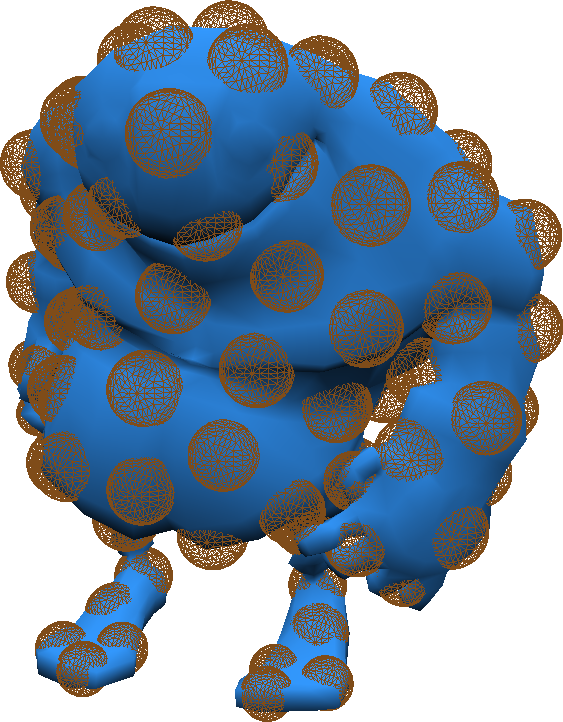
\includegraphics[width=0.4\textwidth]{\rootPath Imgs/precompute_spheres/bigguy_both.png}
		\vspace{0.5cm}
		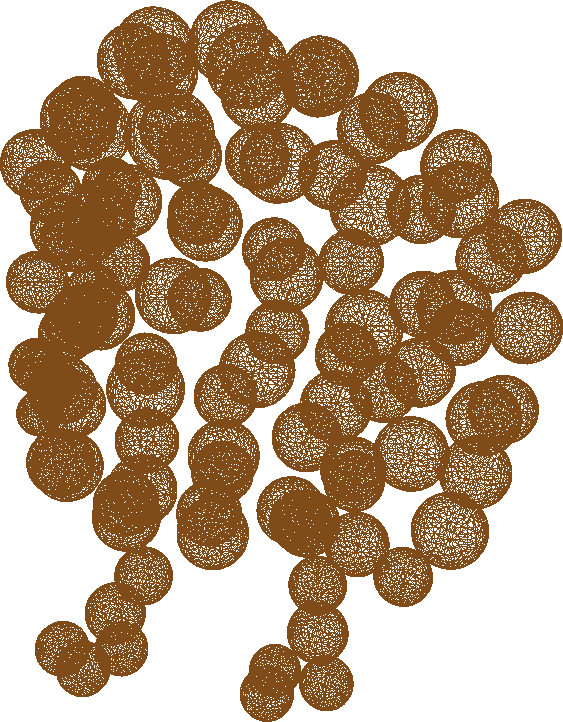
\includegraphics[width=0.4\textwidth]{\rootPath Imgs/precompute_spheres/bigguy_spheres.png}
		\caption{Bigguy (1754 sommets, 2900 triangles)}
	\end{subfigure}
	
	\caption{Décomposition en sphères d'objets 3D ($100000$ échantillons, $100$ sphères)}
	\label{fig:precompute_sphere:result}
\end{figure*}

\subsubsection{Méthode adoptée}

Finalement la solution adoptée, bien que géométriquement pauvre, nous donne des résultats visuellement acceptables tout en garantissant une convergence rapide. L'idée est de paver la surface du maillage à l'aide de sphères de rayon uniforme, ce qui correspond à la minimisation de la distance entre les points et le centre des sphère qui leur sont associés (voir figure~\ref{fig:precompute_sphere:result}).

La distance considérée
\begin{align}
	f(P, S)			&= \left\|P-S\right\|	\\
\intertext{s'optimisant trivialement sur un cluster $C$ par}
	\overline S	&= \left\{ \left(\overline p, \overline{\|p-s\|}\right)\;|\;p \in C \right\}
\end{align}

%=====================================================================
%=====================================================================
\ifstandalone
	\addcontentsline{toc}{chapter}{Bibliographie}
	\bibliographystyle{apalike}
	\bibliography{\rootPath Annexes/biblio}
\fi
%=====================================================================
%=====================================================================
\end{document}
\documentclass[10pt,a4paper,twoside, twocolumn]{report}
%% Lots of packages !
\usepackage{etex}

%% Francisation
\usepackage[francais]{babel}
\usepackage[T1]{fontenc}
\usepackage[utf8]{inputenc}
%\usepackage{textcomp}

%% Réglages généraux
\usepackage[left=1.5cm,right=1.5cm,top=2cm,bottom=2cm]{geometry}
\usepackage{fancyhdr}
\usepackage{setspace}
\usepackage{lscape}
%\usepackage{multicol}
\usepackage{makeidx}
\usepackage[clearempty]{titlesec}
\usepackage{cite}

%% Packages pour le texte
\usepackage{pifont}
\usepackage{eurosym}
\usepackage{soul}
\usepackage[normalem]{ulem}
\usepackage{fancybox}
\usepackage{boxedminipage}
\usepackage{enumerate}
\usepackage{verbatim}
\usepackage{moreverb}
\usepackage{listings}
\usepackage[table]{xcolor}

%% Packages pour les tableaux
\usepackage{array}
\usepackage{multirow}
\usepackage{tabularx}
\usepackage{longtable}

%% Packages pour les dessins
\usepackage{graphicx}
\usepackage{wrapfig}
%\usepackage{picins}
\usepackage{picinpar}
\usepackage{epic}
\usepackage{eepic}
\usepackage{tikz}
\usepackage{afterpage}
\usepackage{rotating}
\usepackage{float}
\usepackage{caption}

%% Packages pour les maths
\usepackage{amsmath}
\usepackage{amssymb}
\usepackage{dsfont}
\usepackage{mathrsfs}
\usepackage{bussproofs}
\usepackage[thmmarks,amsmath]{ntheorem}

%% Création de nouvelles commandes
%\usepackage{calc}
\usepackage{ifthen}
\usepackage{xspace}



\usepackage{url}
\usepackage{hyperref}
\usepackage{todonotes}
\usepackage{subcaption}
\usepackage[french,ruled,vlined,linesnumbered,algochapter,dotocloa]{algorithm2e}
\usepackage{MnSymbol}

\usepackage{chngcntr}

\usepackage{standalone}
\usepackage{import}



\frenchbsetup{StandardEnumerateEnv=true}

%% =======================================================================

\fancypagestyle{empty}{%
  \fancyhf{}
  \fancyhead[L]{}
  \fancyhead[C]{}
  \fancyhead[R]{}
  \fancyfoot[L]{}
  \fancyfoot[C]{}
  \fancyfoot[R]{}
}
\fancypagestyle{basicstyle}{
	\fancyhf{}	
	\fancyhead[L]{}
	\fancyhead[C]{Rendu réaliste et temps réel pour la réalité augmentée}
	\fancyhead[R]{}
	\fancyfoot[L]{hadrien.croubois@ens-lyon.fr}
	\fancyfoot[C]{--~\thepage~--}
	\fancyfoot[R]{}
}
\pagestyle{basicstyle}

%% =======================================================================

\titleformat{\section}[frame]
{\normalfont}
{\filright \footnotesize \enspace Partie \thesection\enspace}
{6pt}
{\bfseries\filcenter}
	
\titleformat{\subsection}[frame]
{\normalfont}
{\filright \footnotesize \enspace \thesubsection\enspace}
{6pt}
{\filcenter}

\titleformat{\subsubsection}
{\titlerule \vspace{.8ex} \normalfont\itshape}
{\thesubsubsection}
{.5em}
{}

\titleformat{\chapter}[display]
{\normalfont\bfseries\filcenter}
{}
{1ex}
{\titlerule[2pt] \vspace{2ex} \LARGE}
[\vspace{1ex} {\titlerule[2pt]}]

\parindent=10pt
\DeclareUnicodeCharacter{00A0}{~}

%% =======================================================================



\newcommand{\HRule}{\rule{\linewidth}{0.5mm}}
\newcommand{\Hs}{\operatorname{HS}}




\floatstyle{ruled}
\restylefloat{figure}
\restylefloat{table}
\newfloat{code}{!h}{locode}{}
\floatname{code}{\textsc{code}}

\addto\captionsfrench{%
  \renewcommand{\listfigurename}{Liste des figures}%
  \renewcommand{\listtablename}{Liste des tableaux}%
  \renewcommand{\listalgorithmcfname}{Liste des algorithmes}%
}
\newcommand{\listofcode}{\listof{code}{Liste des codes}}

\numberwithin{code}{chapter}
\numberwithin{equation}{subsection}
\counterwithout{footnote}{chapter}






\newcommand{\framedgraphics}[2]{%
  \setlength{\fboxsep}{0pt}%
  \setlength{\fboxrule}{1pt}%
  \fbox{\includegraphics[{#1}]{{#2}}}%
}

\newcommand*{\captionsource}[2]{%
  \caption[{#1}]{%
    #1%
    \\\hspace{\linewidth}%
    \textbf{\textsc{Source}} #2%
  }%
}

\newcommand{\footurl}[2][]{\footnote{\textbf{#1}\href{#2}{#2}}}
% \newcommand{\footurl}[2][]{\footnote{\textbf{#1}\url{#2}}}







\newif\iftwocolumn
\twocolumntrue
\usetikzlibrary{3d,arrows, calc, backgrounds, petri, positioning, shadows, shapes}


\tikzset{
	persp/.style={scale=3.0,x={(-0.8cm,-0.4cm)},y={(0.8cm,-0.4cm)}, z={(0cm,1cm)}},
	points/.style={fill=white,draw=black,thick}
	grid/.style={very thin,gray},
	axis/.style={->,ultra thick},
	cube/.style={thick, fill=black!15,opacity=0.5},
	cube hidden/.style={dashed},
	block/.style={
		rectangle, rounded corners,
		draw=black!80,
		fill=black!10, fill opacity=0.5,
		text=black!90, text opacity=1.0,
    text height=1.5ex,
    text depth=.25ex,
    text width=6em,
    text centered
	}
}

\tikzstyle{class}			=[rectangle, rounded corners, draw=black, fill=blue!40, drop shadow, text centered, anchor=north, text=white,    text width=3cm]
\tikzstyle{module}		=[rectangle, rounded corners, draw=black, fill=red!40, 	drop shadow, text centered, anchor=north, text=white,    text width=3cm]
\tikzstyle{component}	=[rectangle, rounded corners, draw=black, fill=green,   drop shadow, text centered, anchor=north, text=black!90, text width=3cm]
\tikzstyle{single}		=[text height=1.5ex, text depth=0.25ex]
\tikzstyle{double}		=[text height=4.0ex, text depth=2.75ex]
\tikzstyle{triple}		=[text height=6.5ex, text depth=5.25ex]
\tikzstyle{quadru}		=[text height=9.0ex, text depth=7.75ex]
\newcommand*{\rootPath}{../}
\standalonetrue

\begin{document}


% \iftwocolumn \onecolumn \else \twocolumn \fi
\onecolumn


\chapter{Résultats et conclusion}


\iftwocolumn \begin{multicols}{2} \fi
En début de stage, nous nous étions fixé l’objectif de développer un pipeline de rendu réaliste, exécutable en temps réel sur des périphériques mobiles, ainsi que de mettre en place les mécanismes nécessaires à l’acquisition dynamique de l’environnement lumineux.

Le travail réalisé nous permet aujourd’hui de proposé une méthode de rendu d’objets 3D dont la principale force est l’utilisation des niveaux de détails des textures pour l’évaluation des intégrations de l’environnement lumineux. Cette approche nous a permis de réaliser non seulement l’éclairage de l’objet mais aussi le rendu d’ombres douces issues de l’objet.
\iftwocolumn \end{multicols} \fi


\begin{figure*}[!ht]\centering

	\begin{subfigure}[b]{0.3\textwidth}\centering
		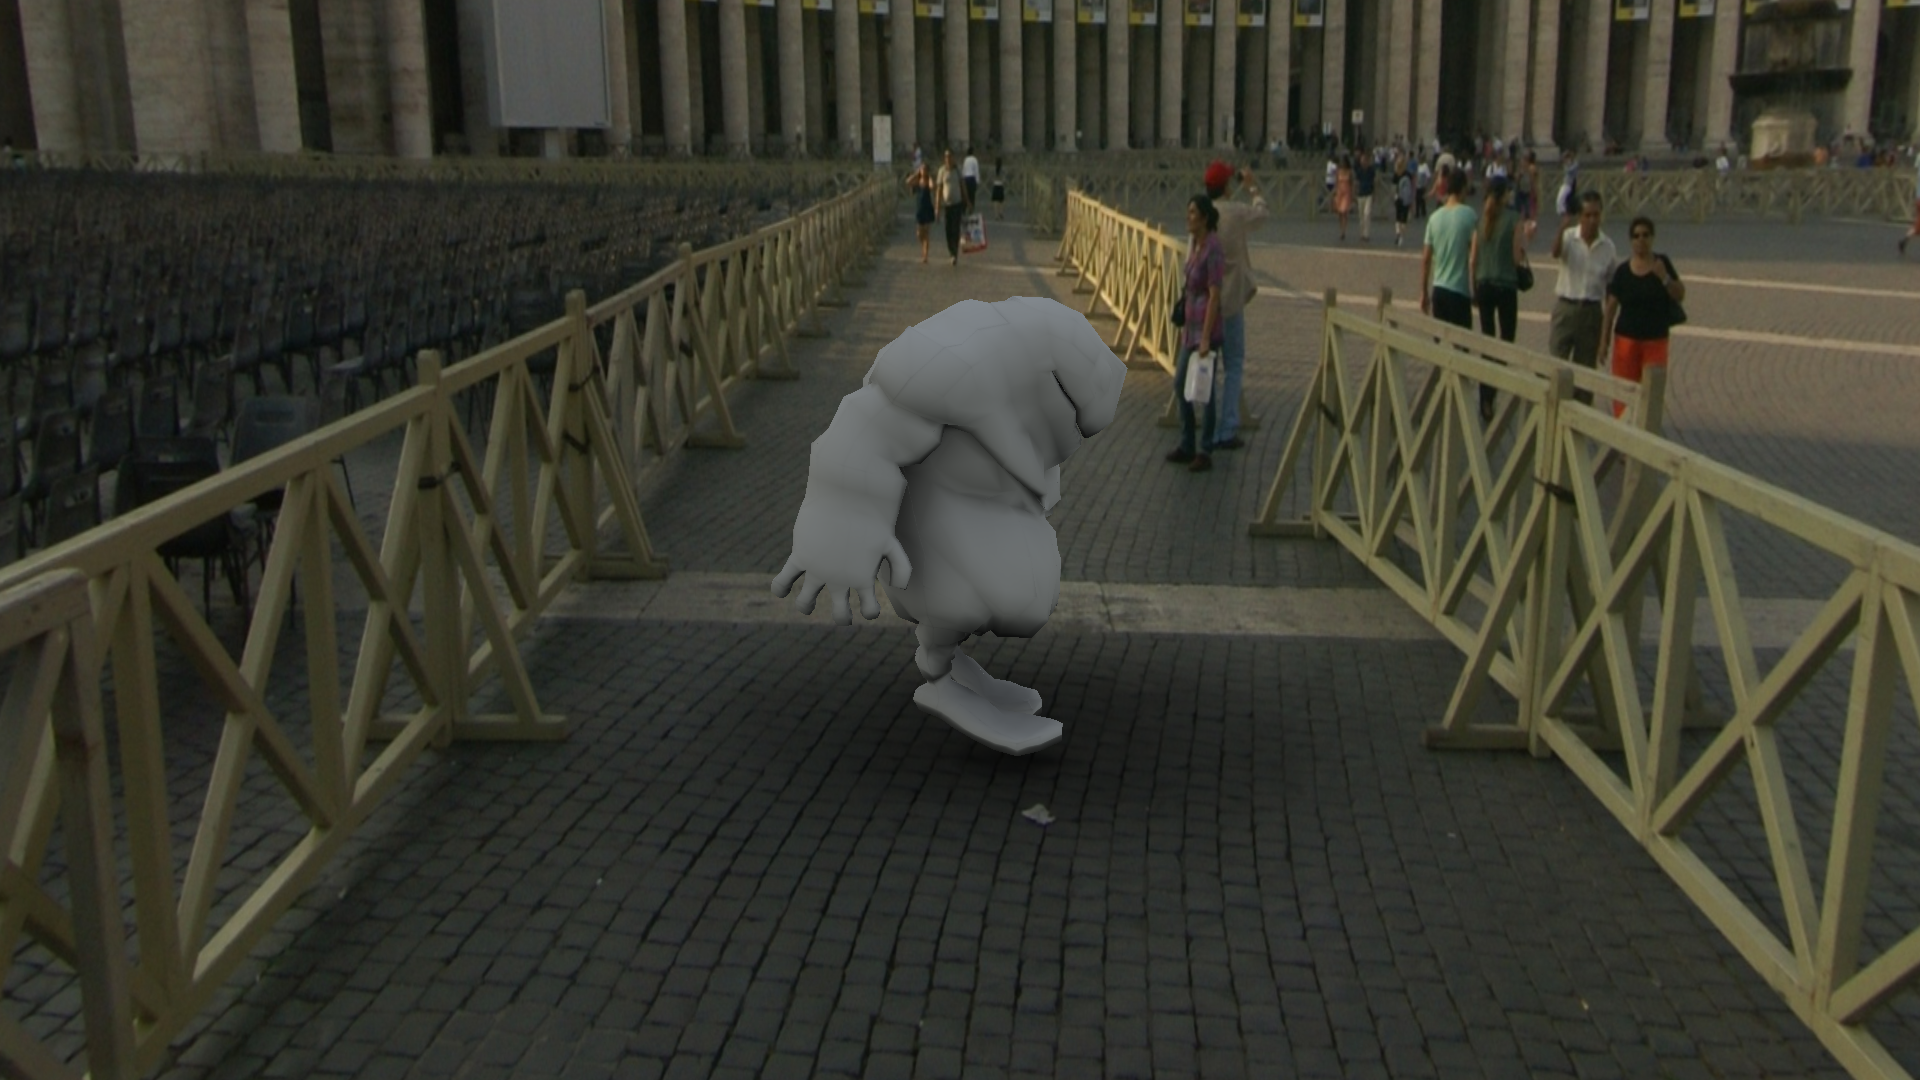
\includegraphics[width=\textwidth]{\rootPath Imgs/screen/white-1.png}
	\end{subfigure}
	\begin{subfigure}[b]{0.3\textwidth}\centering
		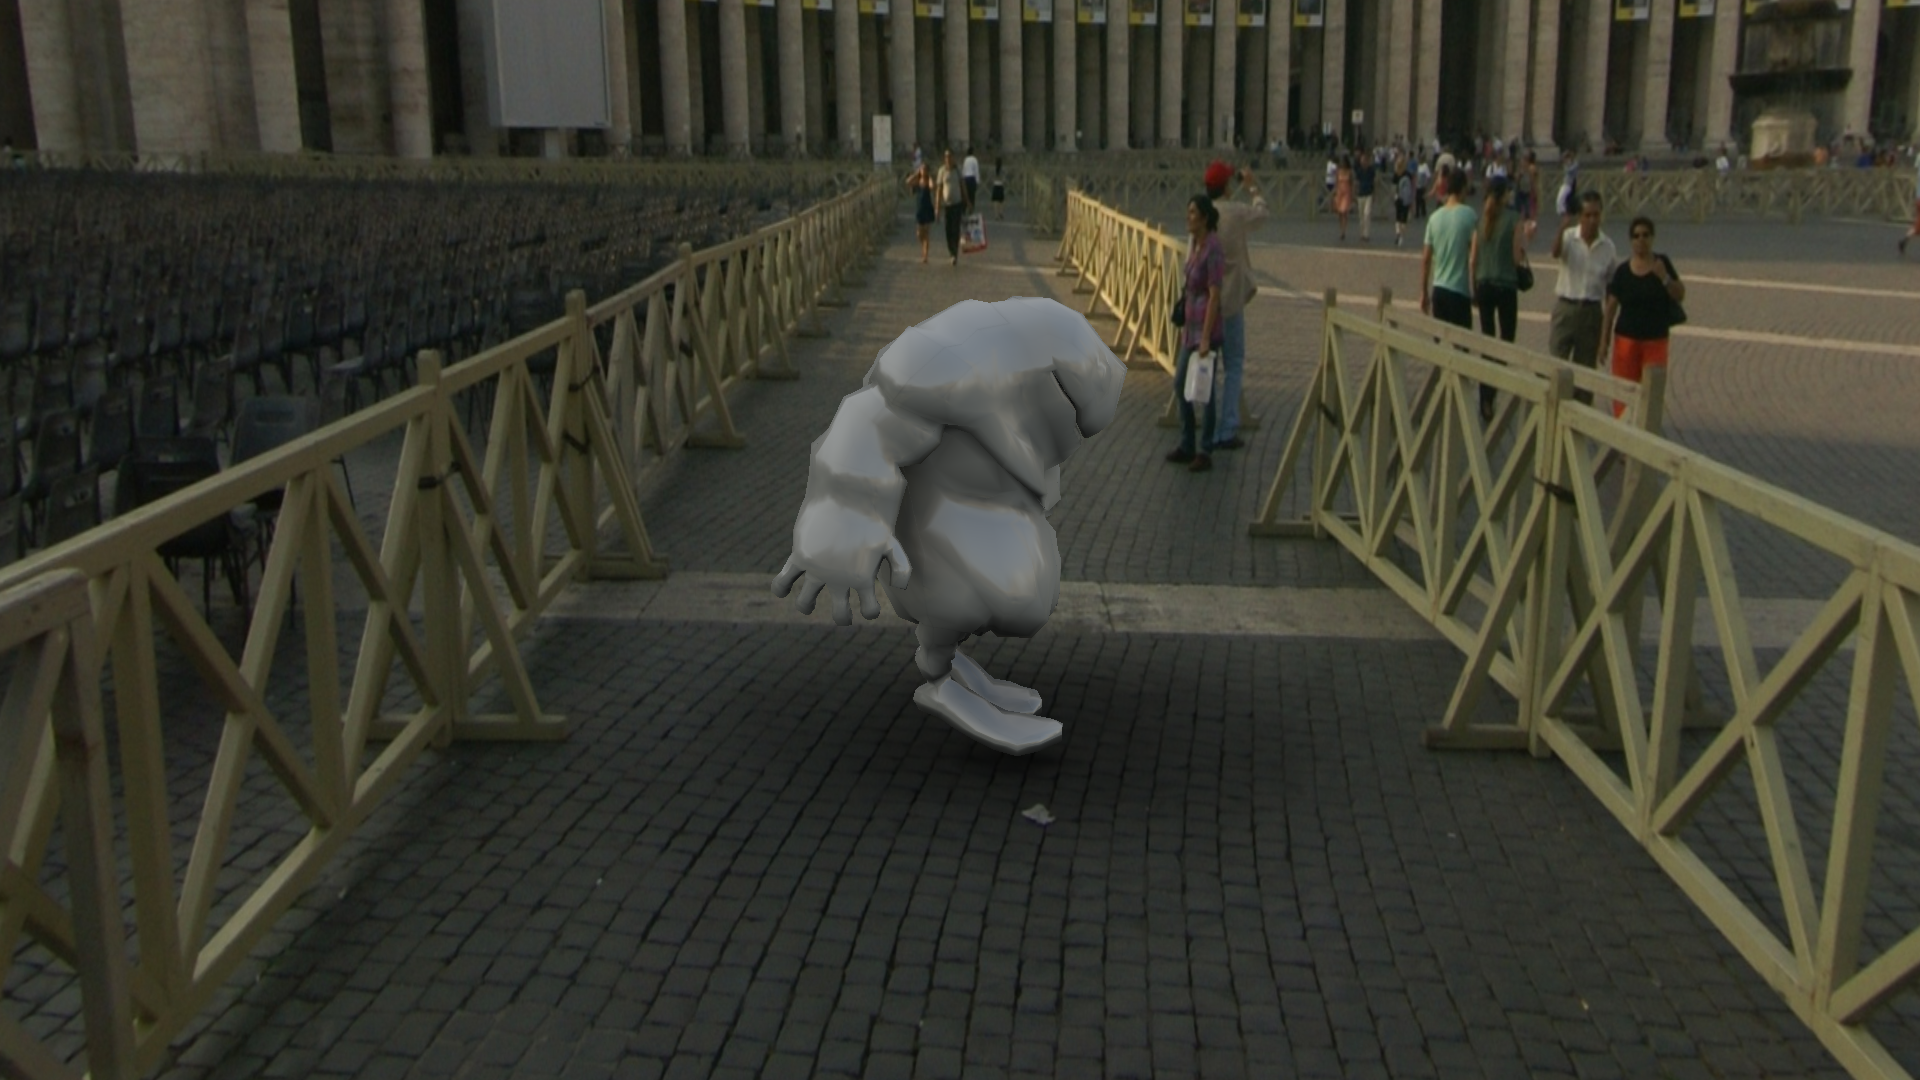
\includegraphics[width=\textwidth]{\rootPath Imgs/screen/glossy-1.png}
	\end{subfigure}
	\begin{subfigure}[b]{0.3\textwidth}\centering
		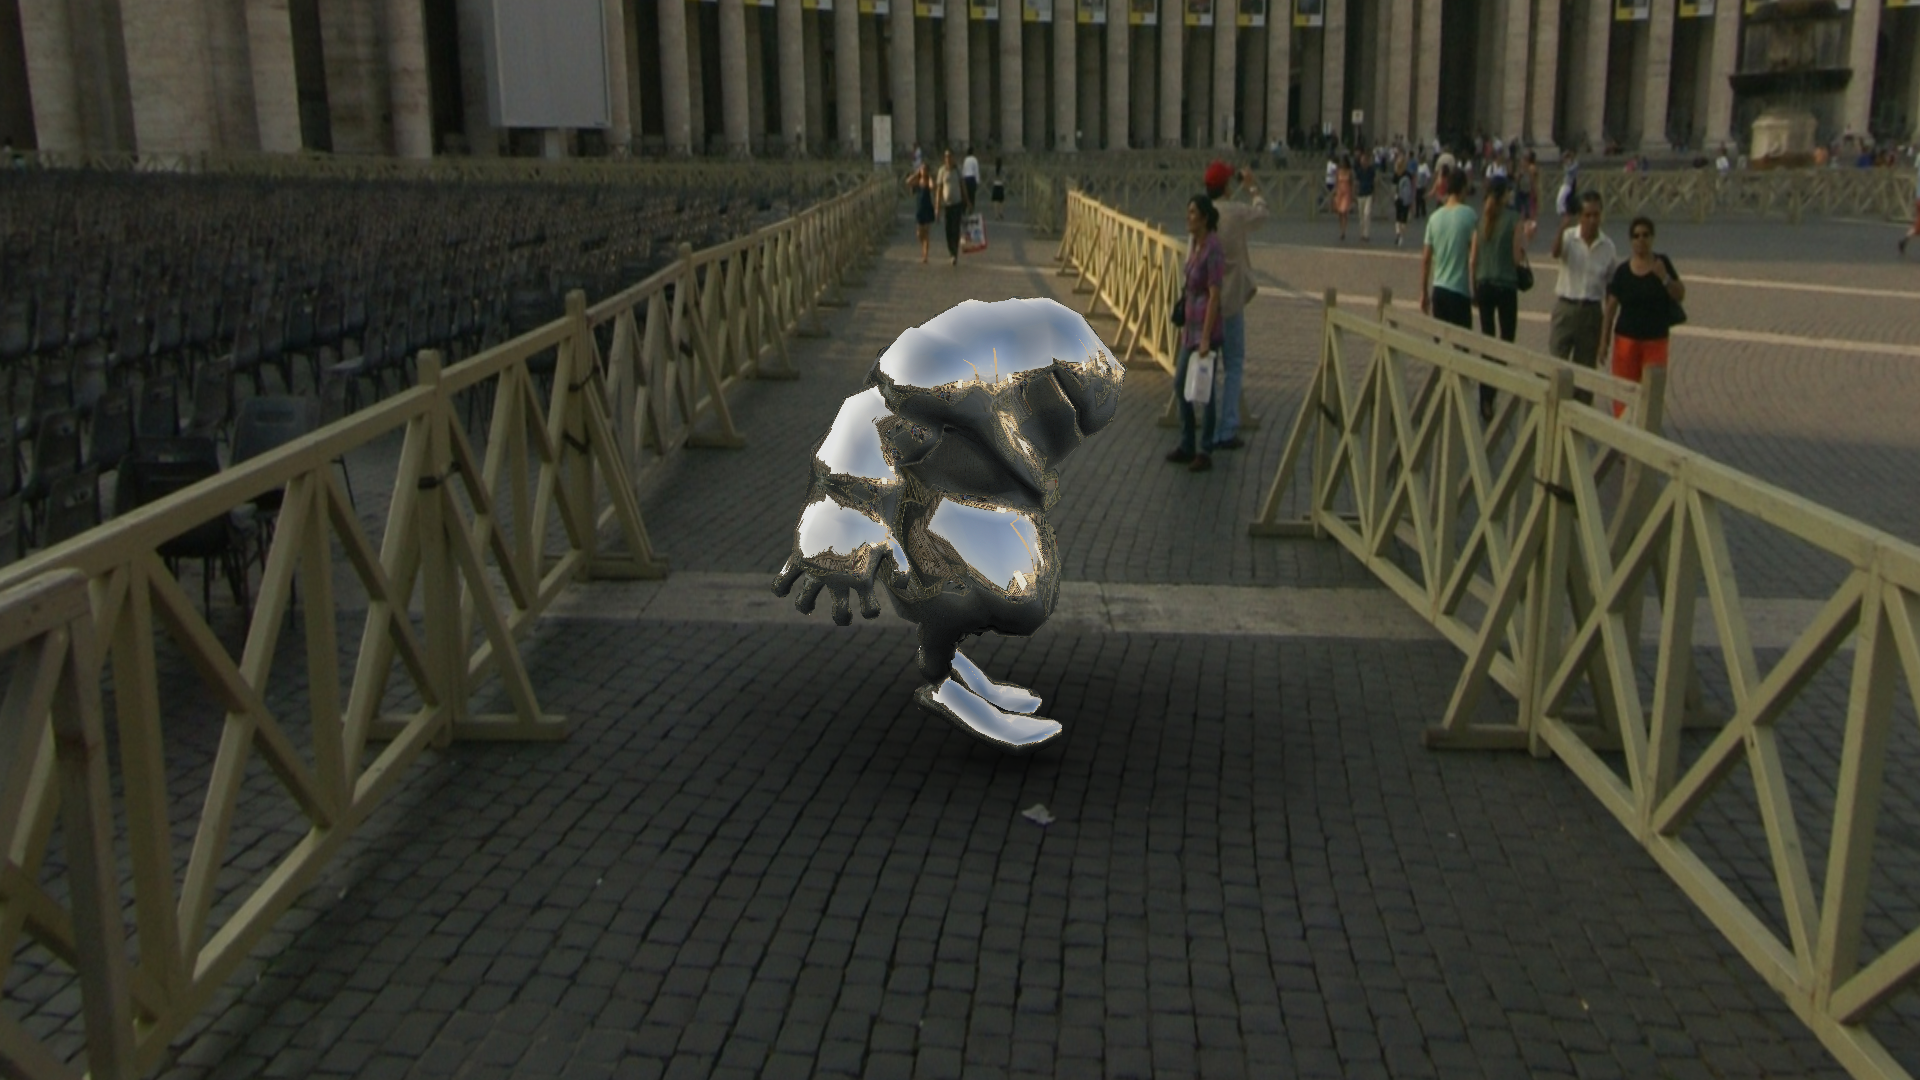
\includegraphics[width=\textwidth]{\rootPath Imgs/screen/miror-1.png}
	\end{subfigure}
	
	\begin{subfigure}[b]{0.3\textwidth}\centering
		\includegraphics[width=\textwidth]{\rootPath Imgs/screen/white-2.png}
	\end{subfigure}
	\begin{subfigure}[b]{0.3\textwidth}\centering
		\includegraphics[width=\textwidth]{\rootPath Imgs/screen/glossy-2.png}
	\end{subfigure}
	\begin{subfigure}[b]{0.3\textwidth}\centering
		\includegraphics[width=\textwidth]{\rootPath Imgs/screen/miror-2.png}
	\end{subfigure}
	
	\begin{subfigure}[b]{0.3\textwidth}\centering
		\includegraphics[width=\textwidth]{\rootPath Imgs/screen/white-3.png}
	\end{subfigure}
	\begin{subfigure}[b]{0.3\textwidth}\centering
		\includegraphics[width=\textwidth]{\rootPath Imgs/screen/glossy-3.png}
	\end{subfigure}
	\begin{subfigure}[b]{0.3\textwidth}\centering
		\includegraphics[width=\textwidth]{\rootPath Imgs/screen/miror-3.png}
	\end{subfigure}
	
	\begin{subfigure}[b]{0.3\textwidth}\centering
		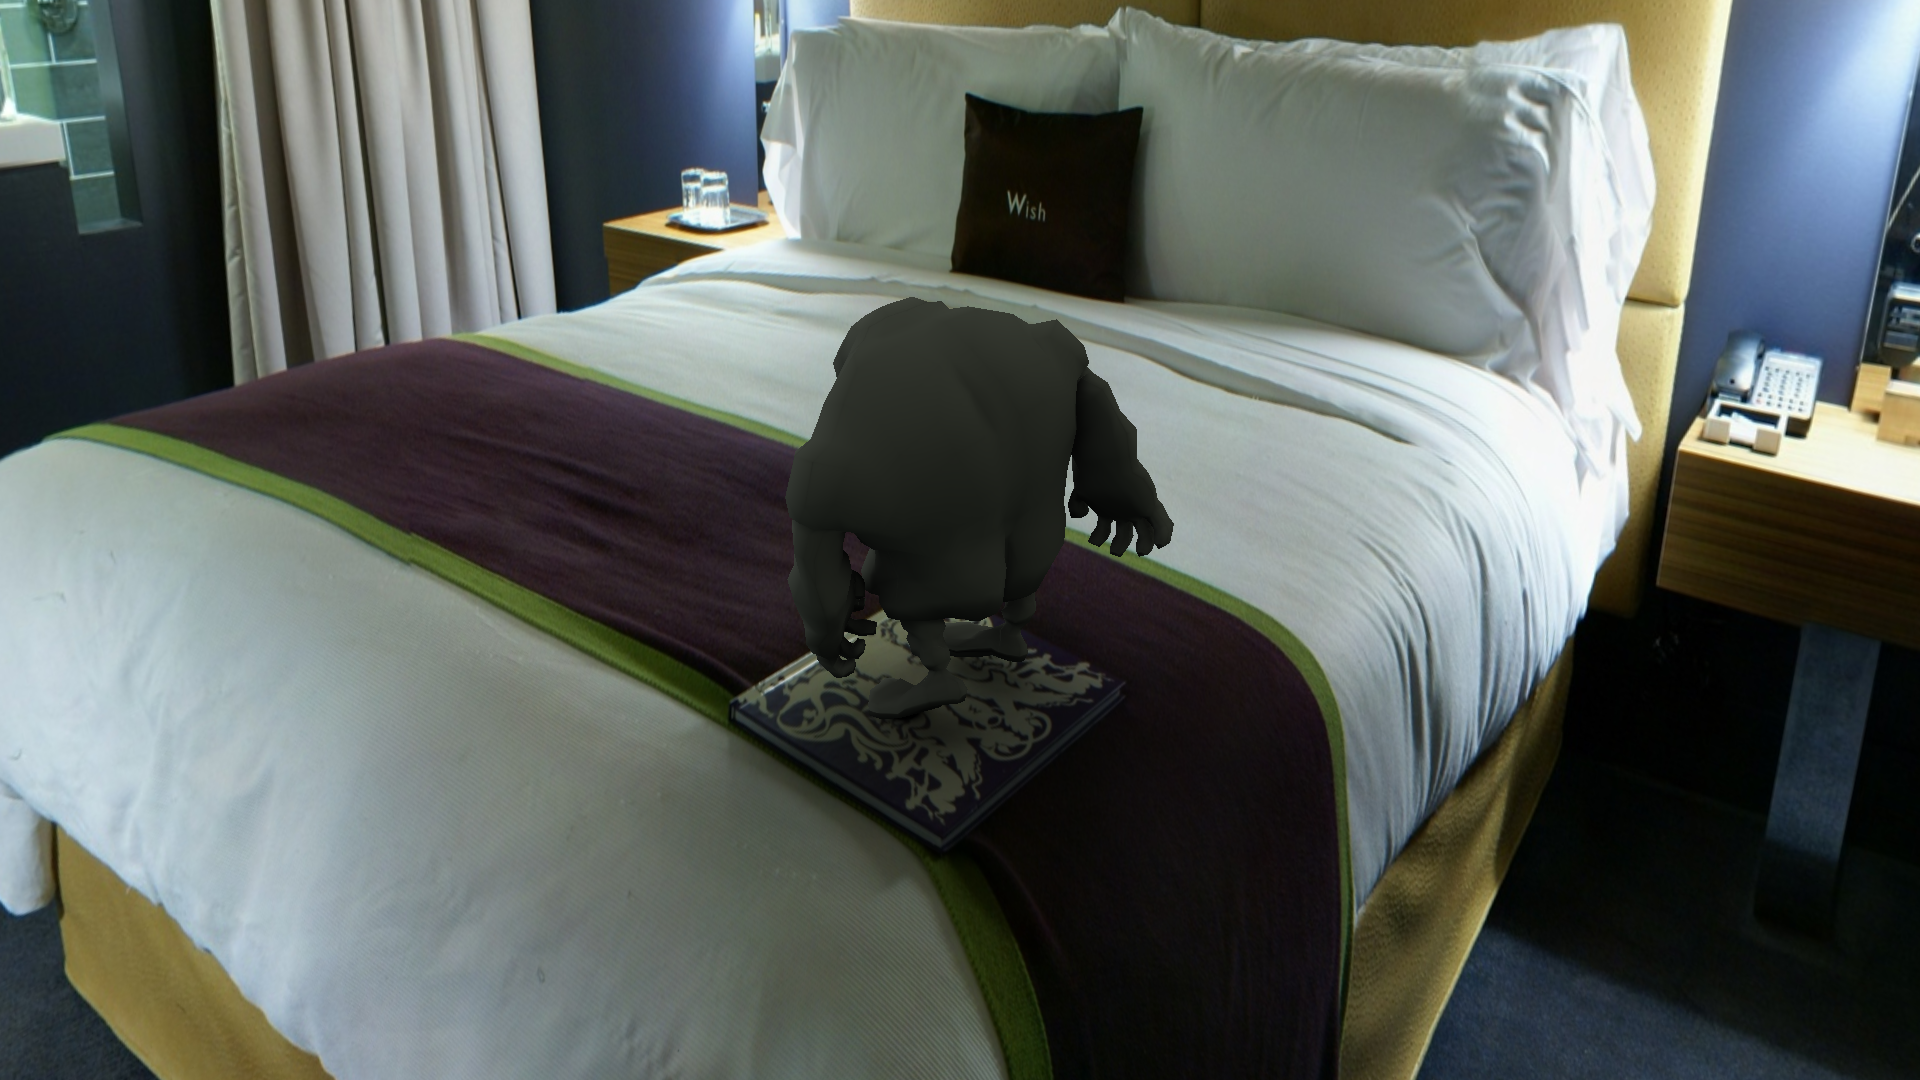
\includegraphics[width=\textwidth]{\rootPath Imgs/screen/white-4.png}
	\end{subfigure}
	\begin{subfigure}[b]{0.3\textwidth}\centering
		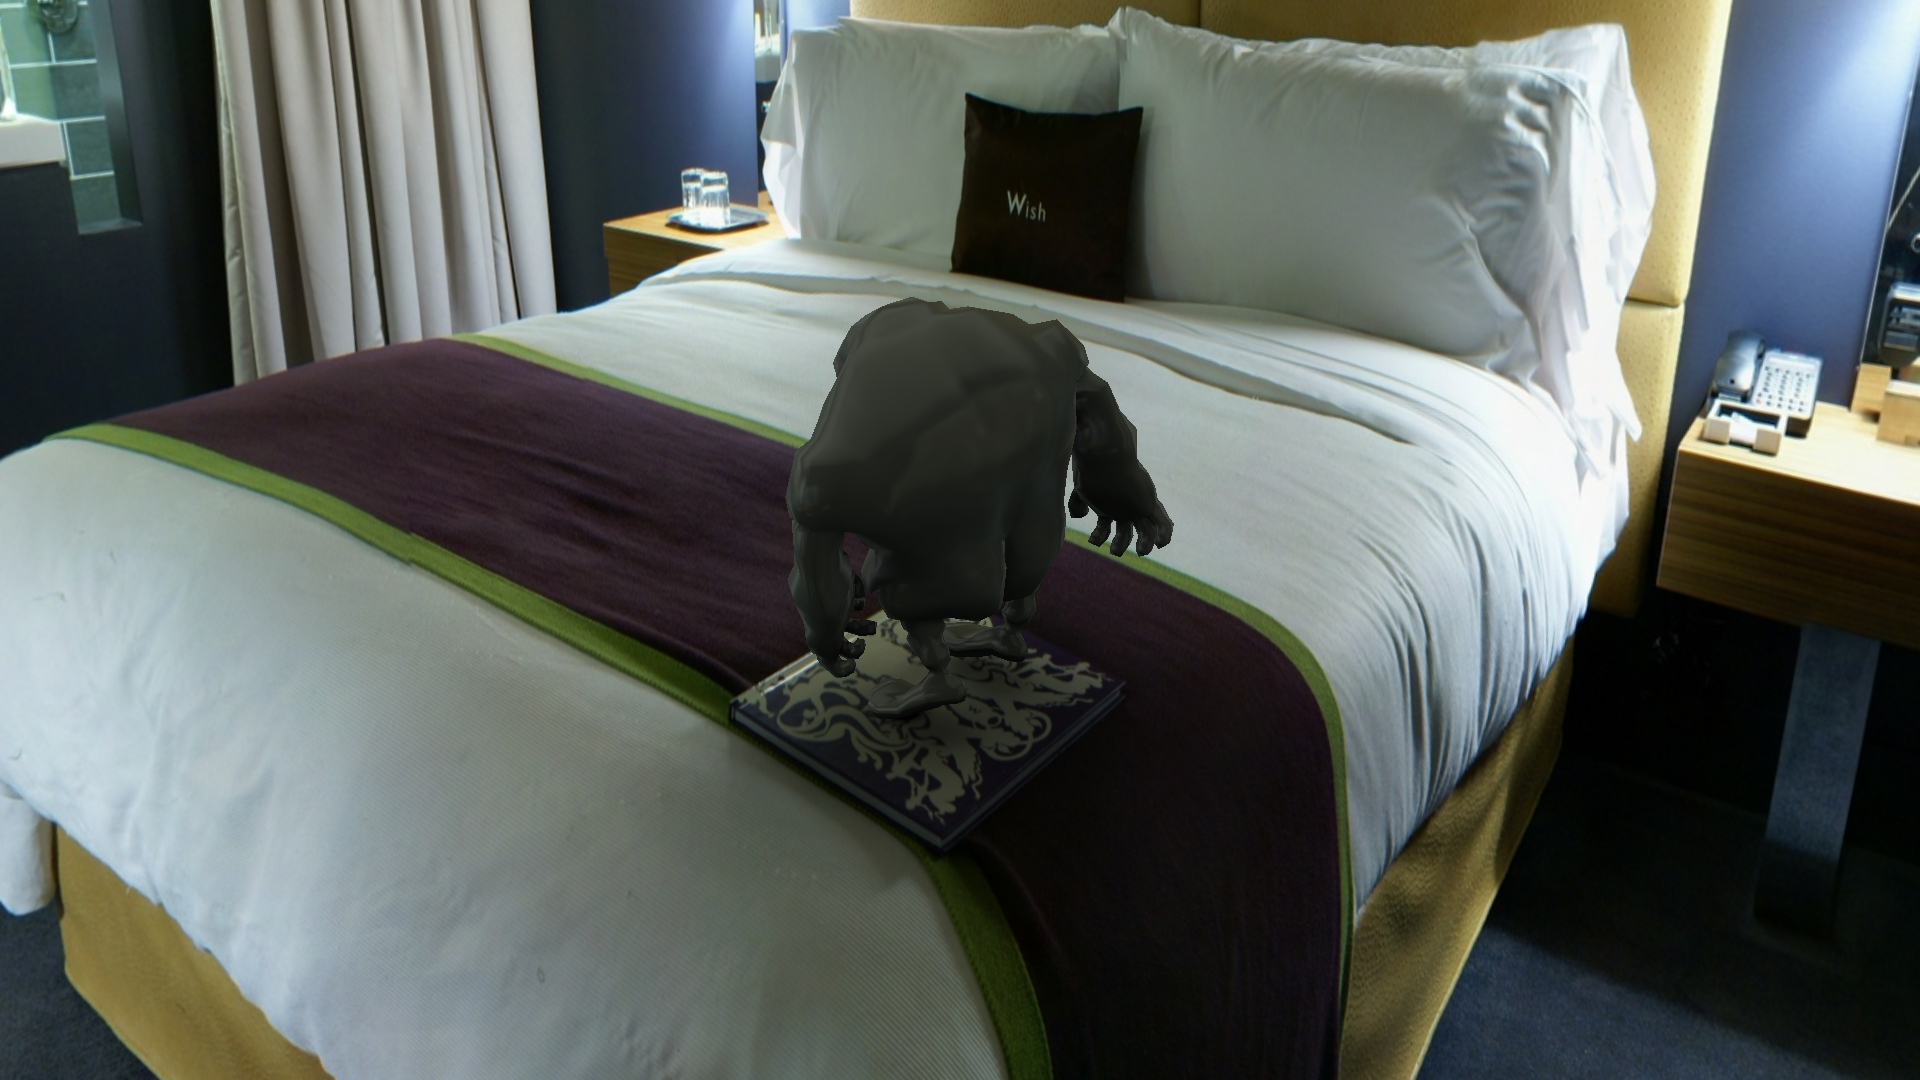
\includegraphics[width=\textwidth]{\rootPath Imgs/screen/glossy-4.png}
	\end{subfigure}
	\begin{subfigure}[b]{0.3\textwidth}\centering
		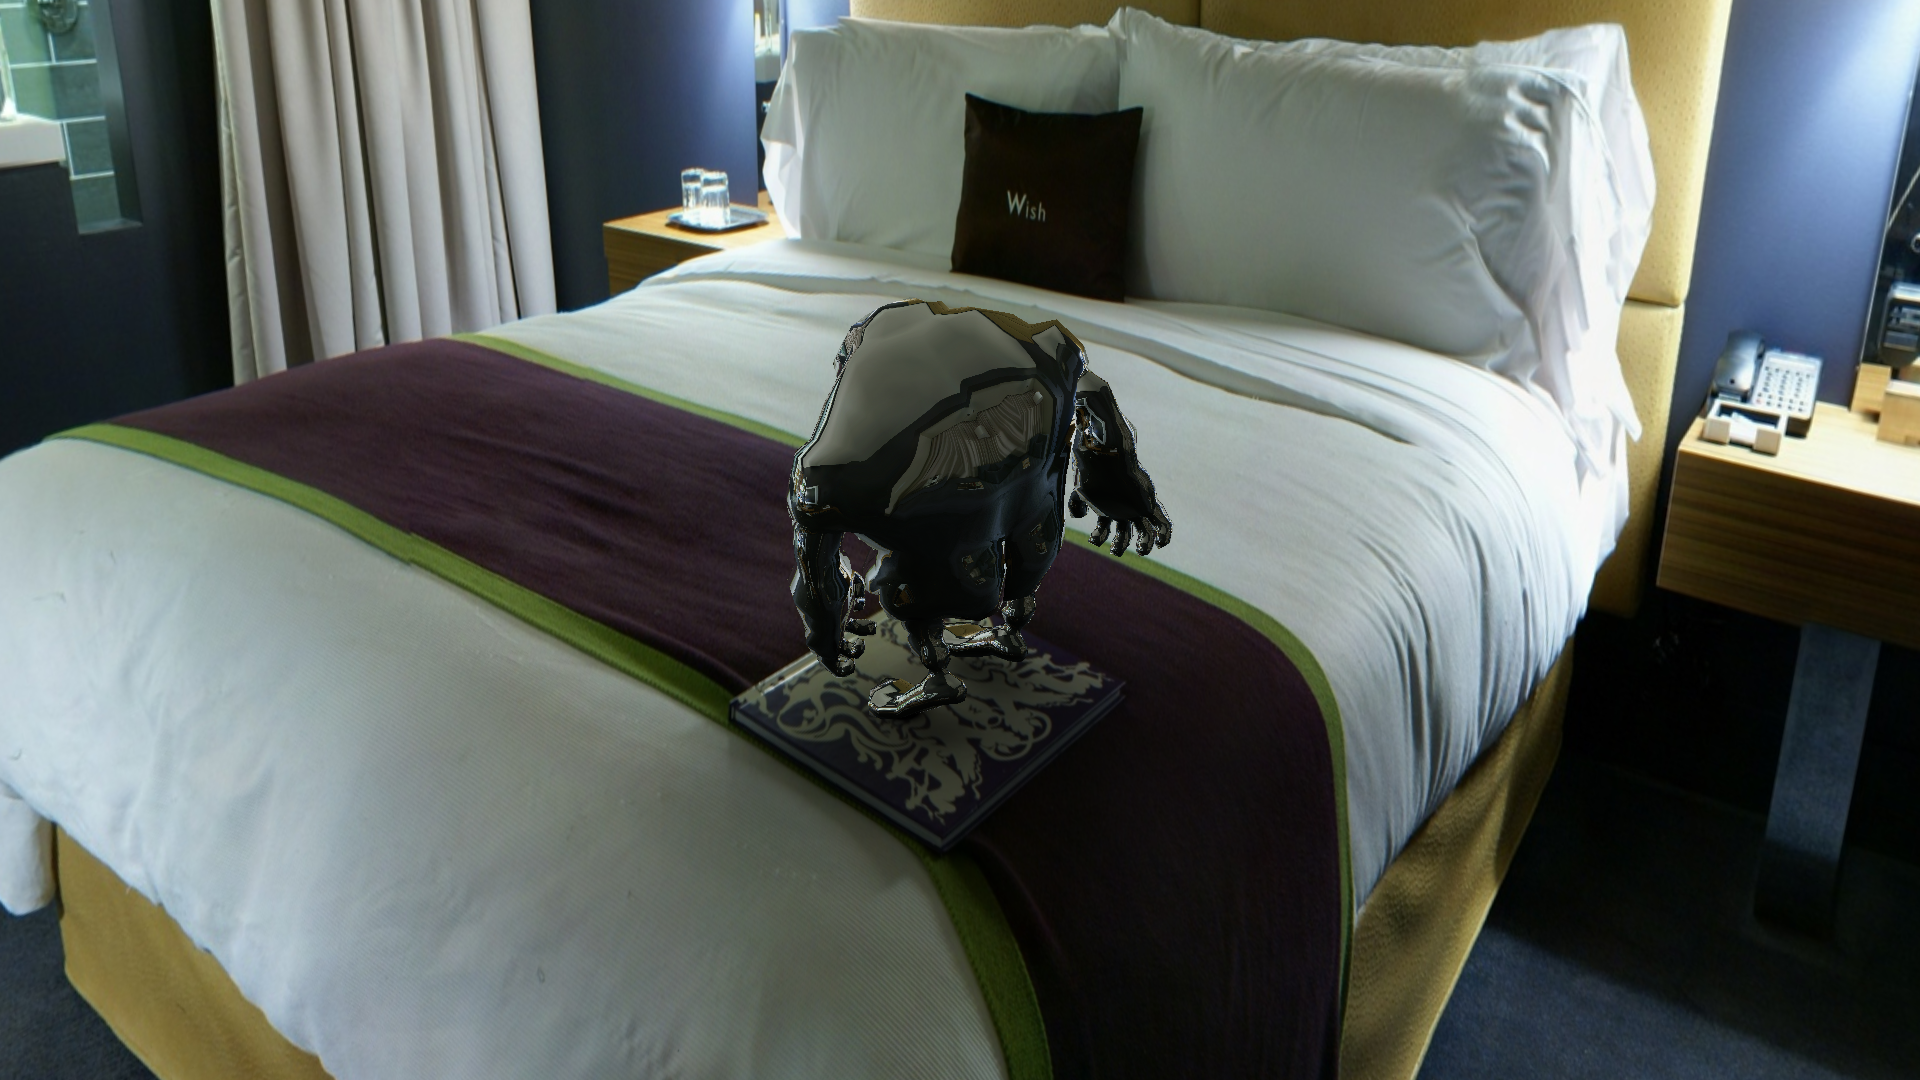
\includegraphics[width=\textwidth]{\rootPath Imgs/screen/miror-4.png}
	\end{subfigure}

	\caption{Rendu du modèle “bigguy” pour differents niveau de spécularité}
	\label{fig:result:specularity}
\end{figure*}


\iftwocolumn \begin{multicols}{2} \fi
L’application développée, ainsi que son portage sur iOS, ont permis de valider le modèle de rendu développée au cours de ce stage. À défaut de correspondre aux résultats d’un modèle statistique, les images rendues répondent aux exigences d’intégration vraisemblable. L’aspect temps réel est lui aussi atteint, les performances sur périphériques mobiles allant de $20$ à plus de $60$ images par seconde selon la méthode d'acquisition de l’envmap. Ces performances sont rendues possible grâce à l’architecture des terminaux mobiles, le fait que la mémoire CPU et GPU soit partagées réduit en effet le coût des transferts mémoire.

Parallèlement, les mécanismes d’acquisition d’envmap développés permettent l’acquisition des données d’environnements nécessaires à la phase de rendu. Même si de nombreux artefacts sont visibles dans le cas de reflets spéculaires, ils restent invisibles pour des matières diffuses. 
\iftwocolumn \end{multicols} \fi


\begin{figure*}[!ht]\centering

	\begin{subfigure}[b]{0.45\textwidth}\centering
		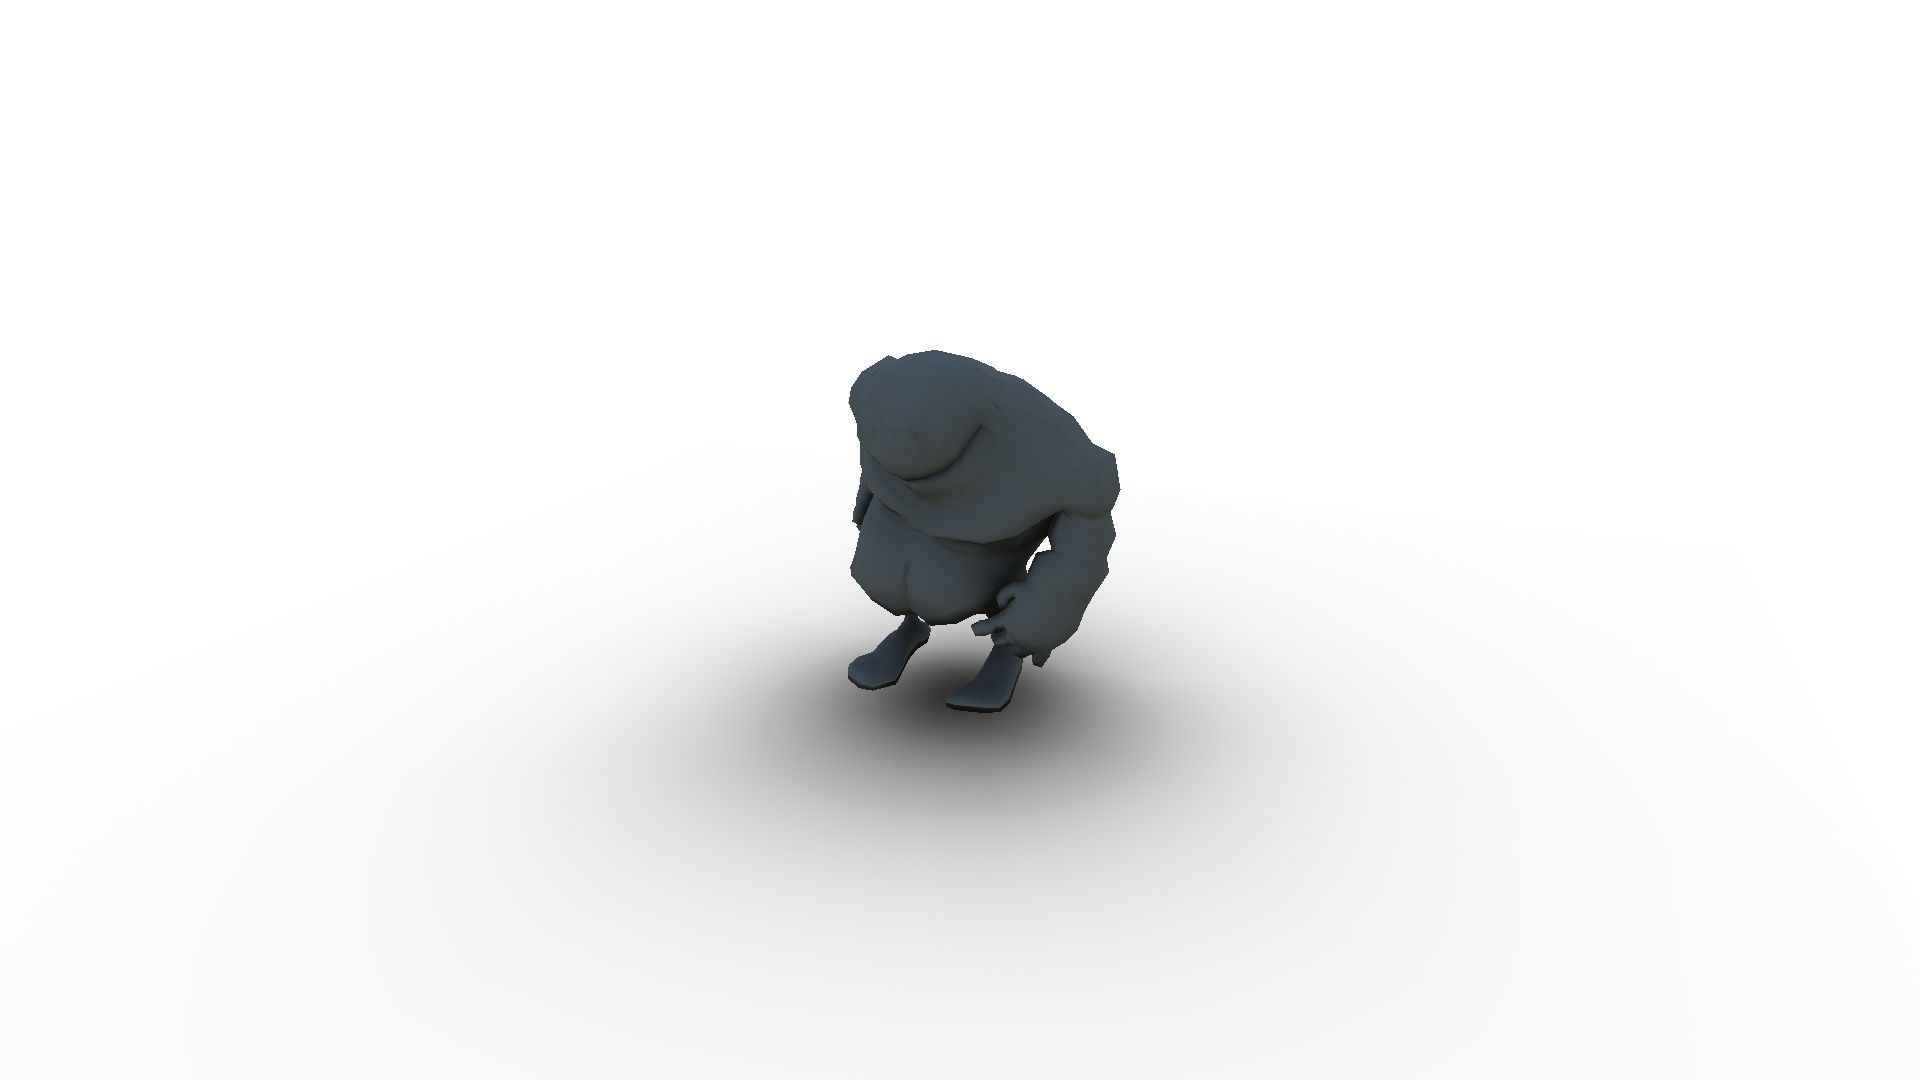
\includegraphics[width=\textwidth]{\rootPath Imgs/screen/sphere-single-1.png}
	\end{subfigure}
	\begin{subfigure}[b]{0.45\textwidth}\centering
		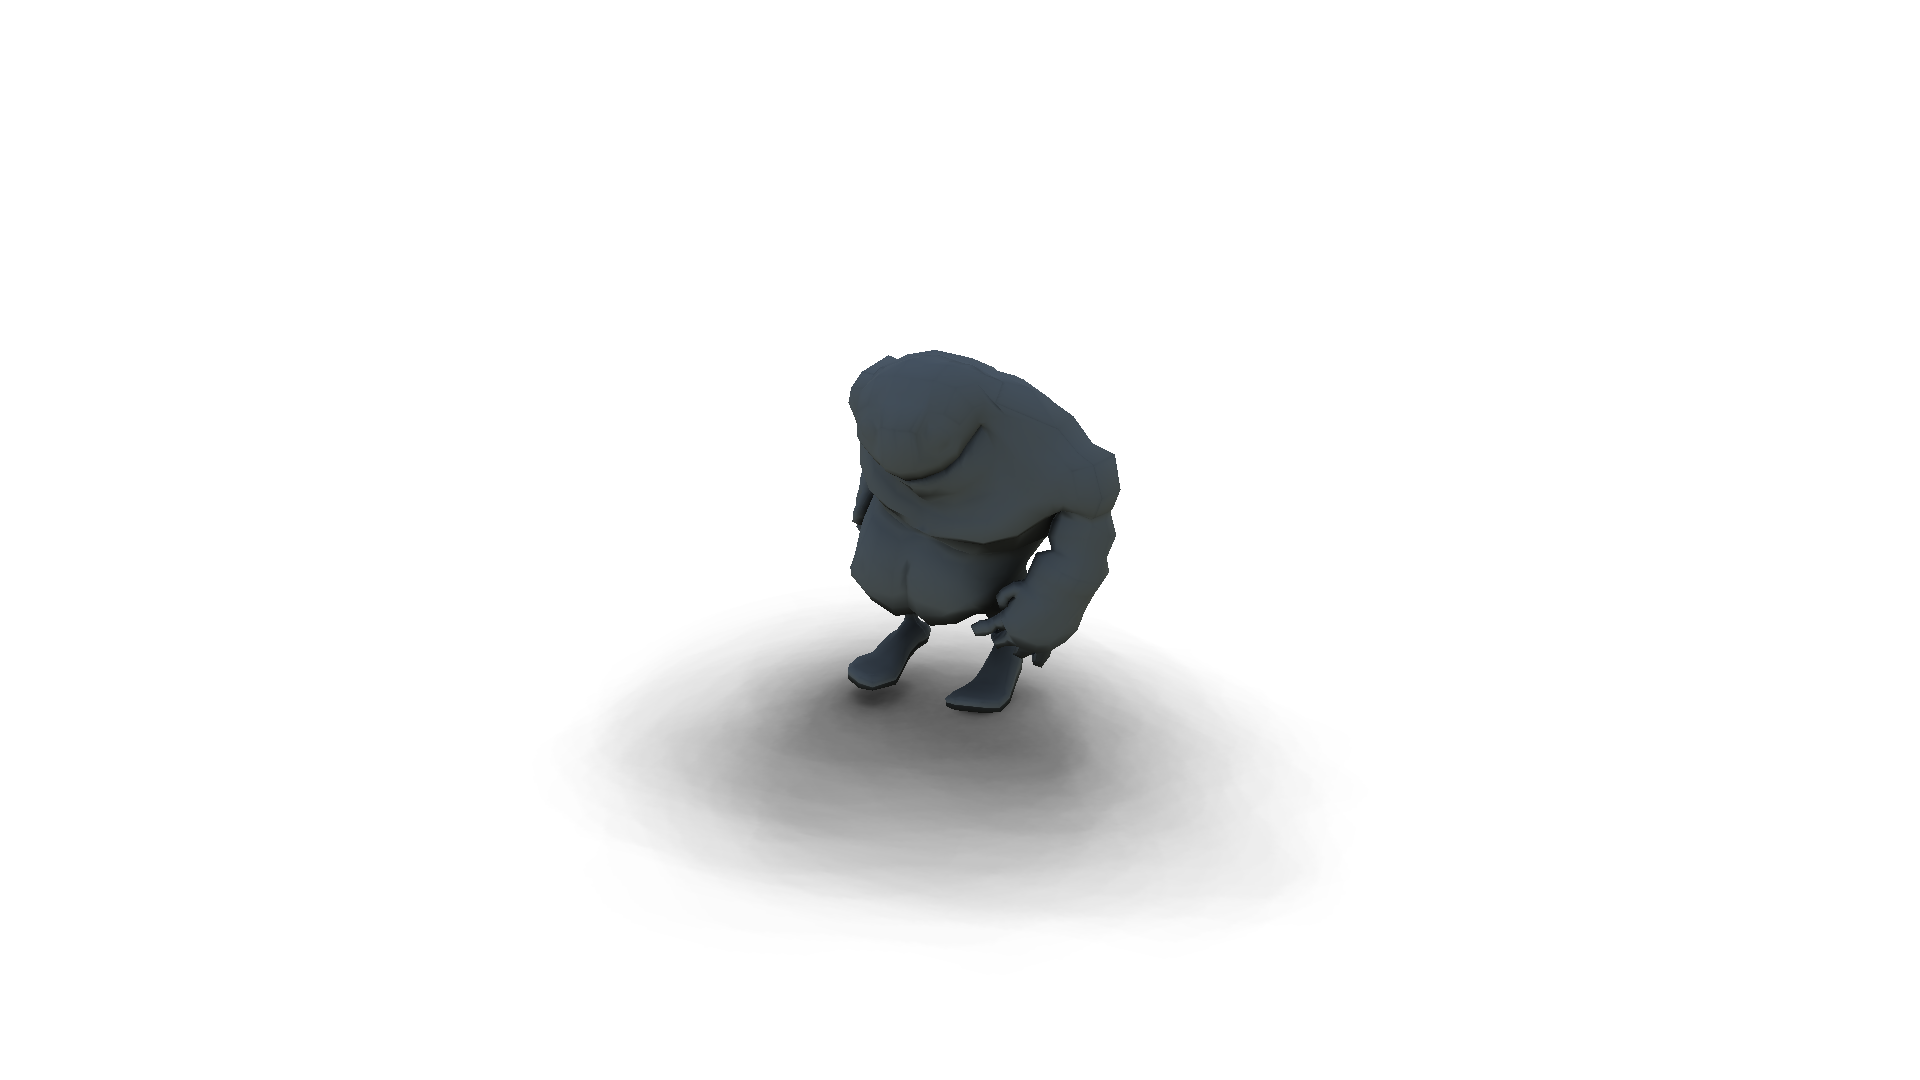
\includegraphics[width=\textwidth]{\rootPath Imgs/screen/sphere-mult-1.png}
	\end{subfigure}
	
	\begin{subfigure}[b]{0.45\textwidth}\centering
		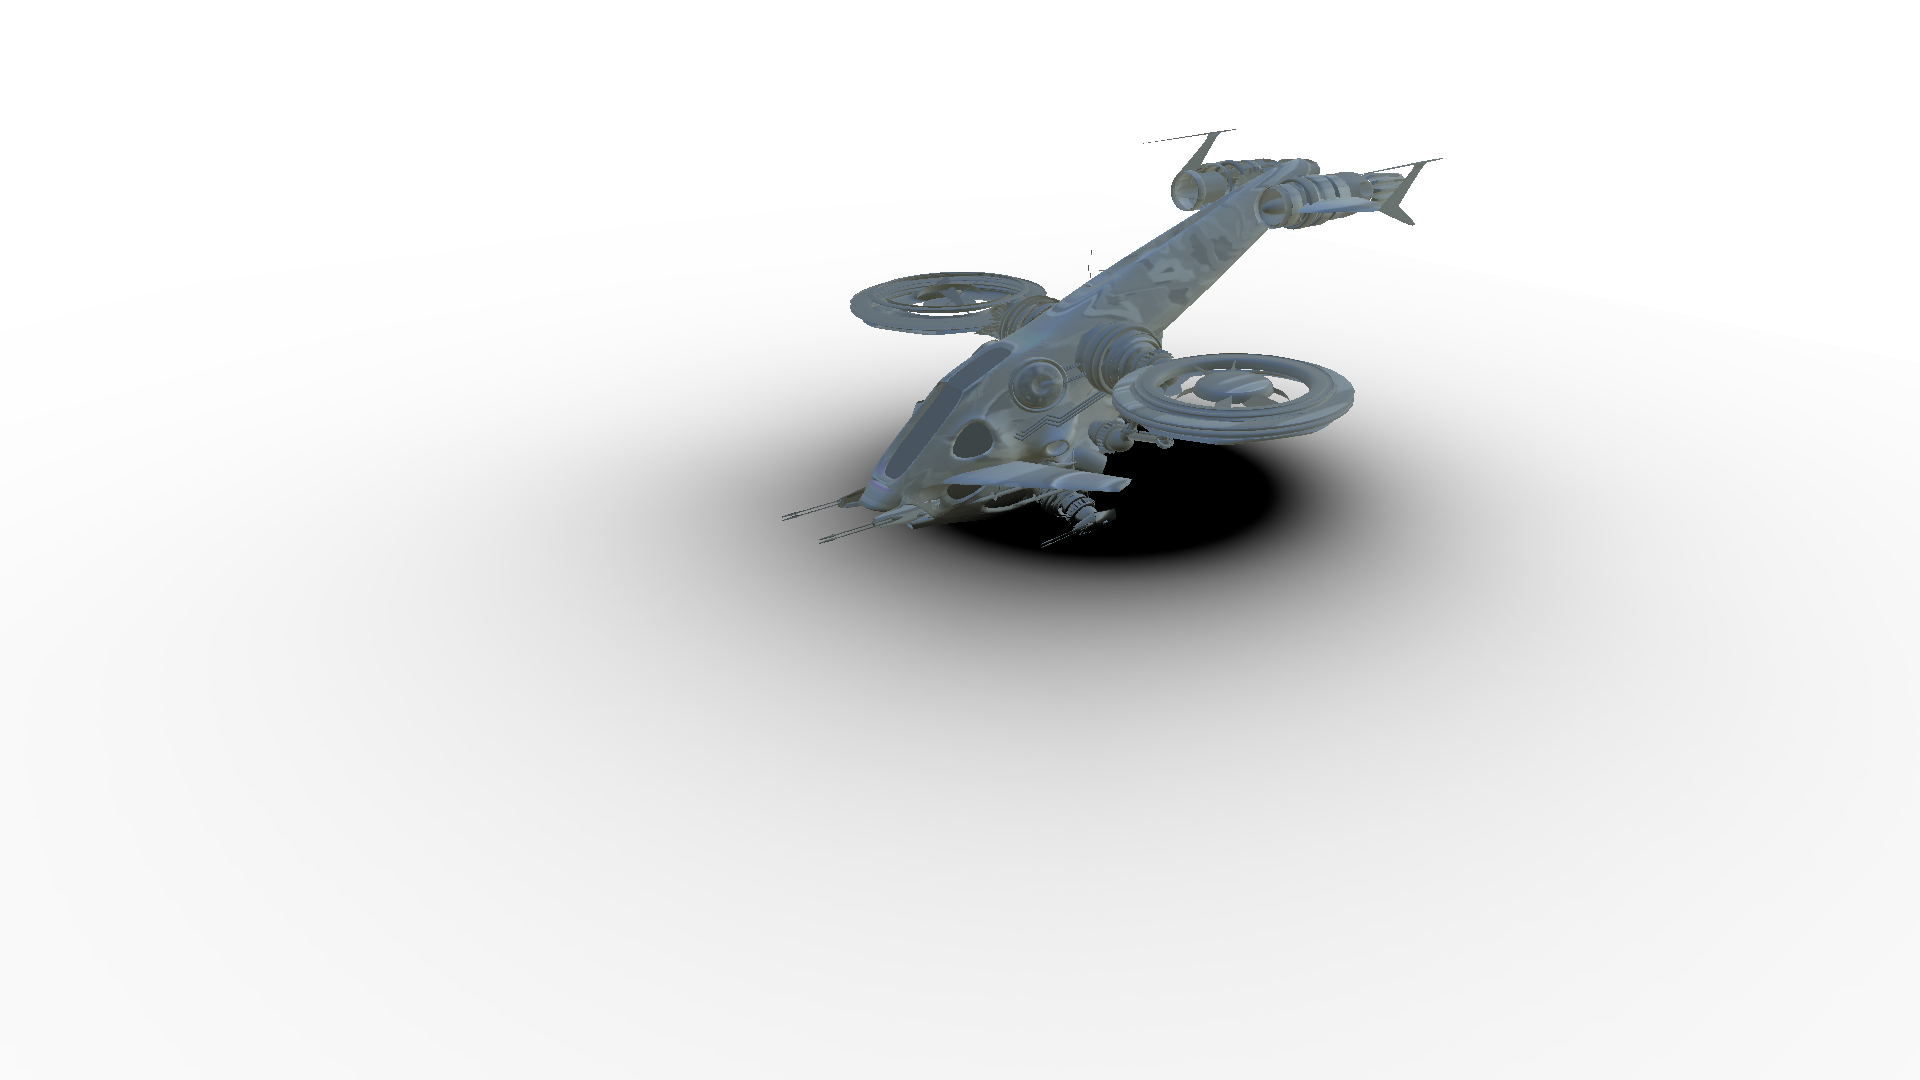
\includegraphics[width=\textwidth]{\rootPath Imgs/screen/sphere-single-2.png}
	\end{subfigure}
	\begin{subfigure}[b]{0.45\textwidth}\centering
		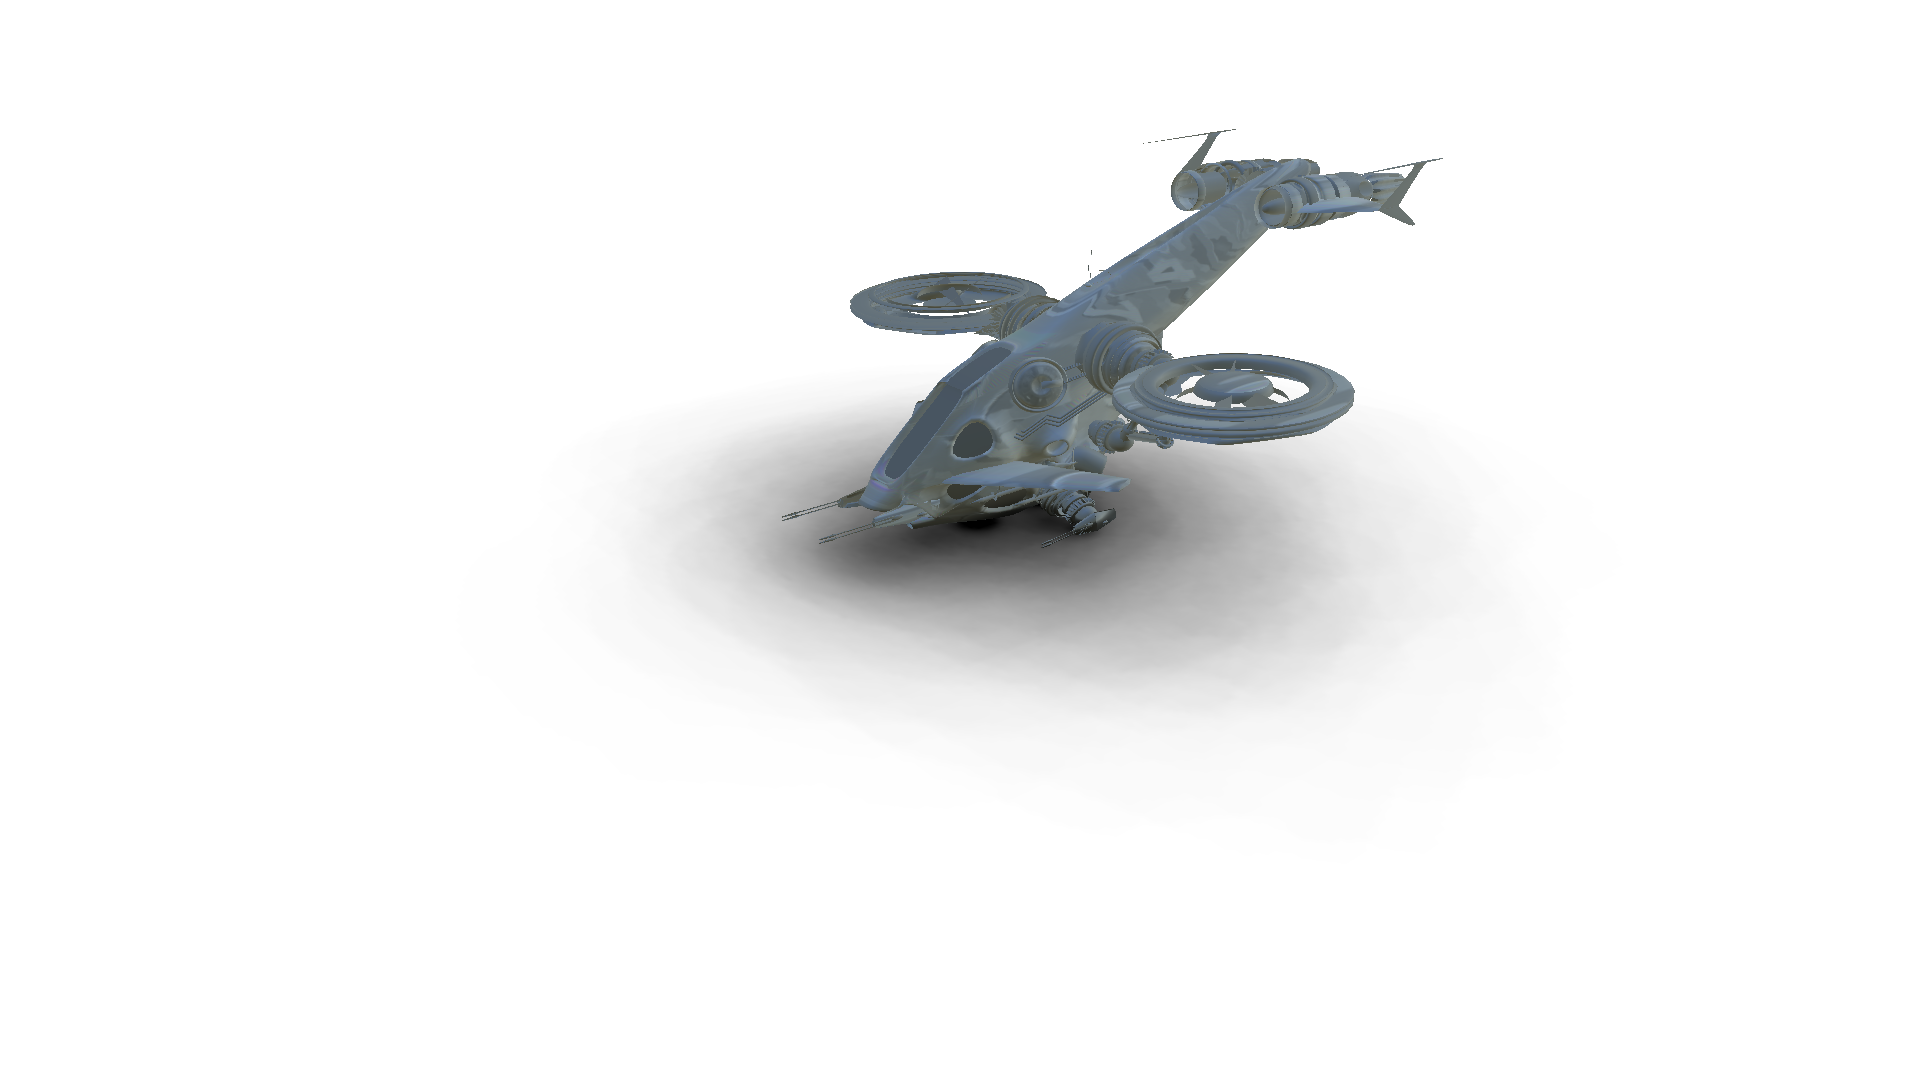
\includegraphics[width=\textwidth]{\rootPath Imgs/screen/sphere-mult-2.png}
	\end{subfigure}
	
	\caption{Rendu des ombres portées sans (gauche) et avec (droite) les informations de sphères englobantes}
	\label{fig:result:spheres}
\end{figure*}


\iftwocolumn \begin{multicols}{2} \fi
Ce portage a permis de confirmer que la génération de terminaux mobiles actuellement sur le marché présente de fait tous les pré-requis, aussi bien matériel que logiciel, nécessaires au développement de la réalité augmentée réaliste et temps réel.

Les méthodes développées sont utilisables dans le développement de nombreuses applications mobiles, notamment pour des fins culturelles (mise en valeur du patrimoine par l’ajout virtuelle d’éléments historiques) ou publicitaires (visualisation d’un objet, d’un meuble ou de vêtements avant achat).
\iftwocolumn \end{multicols} \fi


%=====================================================================
%=====================================================================
\ifstandalone
	\addcontentsline{toc}{chapter}{Bibliographie}
	\bibliographystyle{apalike}
	\bibliography{\rootPath Annexes/biblio}
\fi
%=====================================================================
%=====================================================================
\end{document}
\documentclass[10pt,a4paper,twoside, twocolumn]{report}
%% Lots of packages !
\usepackage{etex}

%% Francisation
\usepackage[francais]{babel}
\usepackage[T1]{fontenc}
\usepackage[utf8]{inputenc}
%\usepackage{textcomp}

%% Réglages généraux
\usepackage[left=1.5cm,right=1.5cm,top=2cm,bottom=2cm]{geometry}
\usepackage{fancyhdr}
\usepackage{setspace}
\usepackage{lscape}
%\usepackage{multicol}
\usepackage{makeidx}
\usepackage[clearempty]{titlesec}
\usepackage{cite}

%% Packages pour le texte
\usepackage{pifont}
\usepackage{eurosym}
\usepackage{soul}
\usepackage[normalem]{ulem}
\usepackage{fancybox}
\usepackage{boxedminipage}
\usepackage{enumerate}
\usepackage{verbatim}
\usepackage{moreverb}
\usepackage{listings}
\usepackage[table]{xcolor}

%% Packages pour les tableaux
\usepackage{array}
\usepackage{multirow}
\usepackage{tabularx}
\usepackage{longtable}

%% Packages pour les dessins
\usepackage{graphicx}
\usepackage{wrapfig}
%\usepackage{picins}
\usepackage{picinpar}
\usepackage{epic}
\usepackage{eepic}
\usepackage{tikz}
\usepackage{afterpage}
\usepackage{rotating}
\usepackage{float}
\usepackage{caption}

%% Packages pour les maths
\usepackage{amsmath}
\usepackage{amssymb}
\usepackage{dsfont}
\usepackage{mathrsfs}
\usepackage{bussproofs}
\usepackage[thmmarks,amsmath]{ntheorem}

%% Création de nouvelles commandes
%\usepackage{calc}
\usepackage{ifthen}
\usepackage{xspace}



\usepackage{url}
\usepackage{hyperref}
\usepackage{todonotes}
\usepackage{subcaption}
\usepackage[french,ruled,vlined,linesnumbered,algochapter,dotocloa]{algorithm2e}
\usepackage{MnSymbol}

\usepackage{chngcntr}

\usepackage{standalone}
\usepackage{import}



\frenchbsetup{StandardEnumerateEnv=true}

%% =======================================================================

\fancypagestyle{empty}{%
  \fancyhf{}
  \fancyhead[L]{}
  \fancyhead[C]{}
  \fancyhead[R]{}
  \fancyfoot[L]{}
  \fancyfoot[C]{}
  \fancyfoot[R]{}
}
\fancypagestyle{basicstyle}{
	\fancyhf{}	
	\fancyhead[L]{}
	\fancyhead[C]{Rendu réaliste et temps réel pour la réalité augmentée}
	\fancyhead[R]{}
	\fancyfoot[L]{hadrien.croubois@ens-lyon.fr}
	\fancyfoot[C]{--~\thepage~--}
	\fancyfoot[R]{}
}
\pagestyle{basicstyle}

%% =======================================================================

\titleformat{\section}[frame]
{\normalfont}
{\filright \footnotesize \enspace Partie \thesection\enspace}
{6pt}
{\bfseries\filcenter}
	
\titleformat{\subsection}[frame]
{\normalfont}
{\filright \footnotesize \enspace \thesubsection\enspace}
{6pt}
{\filcenter}

\titleformat{\subsubsection}
{\titlerule \vspace{.8ex} \normalfont\itshape}
{\thesubsubsection}
{.5em}
{}

\titleformat{\chapter}[display]
{\normalfont\bfseries\filcenter}
{}
{1ex}
{\titlerule[2pt] \vspace{2ex} \LARGE}
[\vspace{1ex} {\titlerule[2pt]}]

\parindent=10pt
\DeclareUnicodeCharacter{00A0}{~}

%% =======================================================================



\newcommand{\HRule}{\rule{\linewidth}{0.5mm}}
\newcommand{\Hs}{\operatorname{HS}}




\floatstyle{ruled}
\restylefloat{figure}
\restylefloat{table}
\newfloat{code}{!h}{locode}{}
\floatname{code}{\textsc{code}}

\addto\captionsfrench{%
  \renewcommand{\listfigurename}{Liste des figures}%
  \renewcommand{\listtablename}{Liste des tableaux}%
  \renewcommand{\listalgorithmcfname}{Liste des algorithmes}%
}
\newcommand{\listofcode}{\listof{code}{Liste des codes}}

\numberwithin{code}{chapter}
\numberwithin{equation}{subsection}
\counterwithout{footnote}{chapter}






\newcommand{\framedgraphics}[2]{%
  \setlength{\fboxsep}{0pt}%
  \setlength{\fboxrule}{1pt}%
  \fbox{\includegraphics[{#1}]{{#2}}}%
}

\newcommand*{\captionsource}[2]{%
  \caption[{#1}]{%
    #1%
    \\\hspace{\linewidth}%
    \textbf{\textsc{Source}} #2%
  }%
}

\newcommand{\footurl}[2][]{\footnote{\textbf{#1}\href{#2}{#2}}}
% \newcommand{\footurl}[2][]{\footnote{\textbf{#1}\url{#2}}}







\newif\iftwocolumn
\twocolumntrue
\usetikzlibrary{3d,arrows, calc, backgrounds, petri, positioning, shadows, shapes}


\tikzset{
	persp/.style={scale=3.0,x={(-0.8cm,-0.4cm)},y={(0.8cm,-0.4cm)}, z={(0cm,1cm)}},
	points/.style={fill=white,draw=black,thick}
	grid/.style={very thin,gray},
	axis/.style={->,ultra thick},
	cube/.style={thick, fill=black!15,opacity=0.5},
	cube hidden/.style={dashed},
	block/.style={
		rectangle, rounded corners,
		draw=black!80,
		fill=black!10, fill opacity=0.5,
		text=black!90, text opacity=1.0,
    text height=1.5ex,
    text depth=.25ex,
    text width=6em,
    text centered
	}
}

\tikzstyle{class}			=[rectangle, rounded corners, draw=black, fill=blue!40, drop shadow, text centered, anchor=north, text=white,    text width=3cm]
\tikzstyle{module}		=[rectangle, rounded corners, draw=black, fill=red!40, 	drop shadow, text centered, anchor=north, text=white,    text width=3cm]
\tikzstyle{component}	=[rectangle, rounded corners, draw=black, fill=green,   drop shadow, text centered, anchor=north, text=black!90, text width=3cm]
\tikzstyle{single}		=[text height=1.5ex, text depth=0.25ex]
\tikzstyle{double}		=[text height=4.0ex, text depth=2.75ex]
\tikzstyle{triple}		=[text height=6.5ex, text depth=5.25ex]
\tikzstyle{quadru}		=[text height=9.0ex, text depth=7.75ex]
\newcommand*{\rootPath}{../}
\standalonetrue

\begin{document}


\iftwocolumn \twocolumn \else \onecolumn \fi


\chapter{Perspectives d’évolution}

Au delà des travaux développés au cours de ce stage, certains aspect sont encore en travaux. Les problématiques discutées dans ce chapitre sont sujet à modifications et pourrait faire l’objet de nouveaux travaux dans ma continuité des résultats déjà obtenus.


\section{Acquisition HDR}

La méthode de rendu développée utilise les informations le luminosité de la scène. Ces informations, issues de camera standard, ne traduisent pas la réalité physique de la luminosité de la scène mais plutôt la perception que l’on peut avoir de cette scène. Les données obtenus par le capteur photosensible sont en effet traités pour obtenir une image classique.

L’imagerie HDR\footurl[HDR:~]{http://en.wikipedia.org/wiki/High-dynamic-range\_imaging} (High dynamic range), par opposition aux images classique ou LDR (Low dynamic range), vise à considérer une dynamique de luminosité plus large qui permettent de représenter les contrastes présent dans la nature. 

Les calculs d’éclairement développée dans ce rapport étant fait du point de vue de l’intensité lumineuse reçu par unité de surface, il faudrait théoriquement les appliquer à une envmap HDR qui reflètent les fortes différences de luminosité présentes dans la scène. Cela implique d’acquérir, en temps réel, une vue HDR de la scène. 

Les méthodes d’acquisition HDR nécessite généralement plusieurs prise de vues avec différentes expositions qui sont par la suite fusionnées en un unique image HDR. D’autres méthodes proposent, à défaut d’un grand nombres de prise de vue, d’utiliser différentes heuristiques pour reconstruire une image HDR à partir d’une unique image LDR\cite{Rempel2006}.

L’utilisation d’une envmap devrait améliorer les résultats de rendu, notamment pour des scènes présentant de forts contrastes. Le modèle d’ombre douce présenté plus tôt devrai par ailleurs, avec une telle envmap, permettre de reconstruire des ombres assez dures dans le cas d’une source principale comme le soleil.

La principale difficultés viens de la reconstruction de l’image HDR en temps réel, notamment avec des cameras ne permettant pas de régler ou même de fixer les paramètres d’exposition. L’étape de calibration des cameras d’être une étape difficile. 

La version $3.0$ d’OpenCV\footurl[OpenCV:~]{http://opencv.org/} devrait voir l’apparition d’outils pour la reconstruction et la manipulation d’images HDR. Il semble intéressant, une fois cette mise a jour disponible, d’étudier les possibilités offertes pour éventuellement les intégrer au module d’acquisition \texttt{videodevice\_opencv}.


\section{BRDF anisotropes}

Une des possibilités perspectives évoquées dans la section rendu est la possibilités de considérer un modèle de surface à micro-facettes.

Un tel modèle, étoffé d’informations surfacique décrivant la distribution de micro-facettes permet un rendu réaliste de matières anisotropes comme le métal brossé.

Pour cela de lourds calcules statistiques sont nécessaires dans l’évaluation de la direction de réflexion étant donné l’angle de vue et les caractéristiques de la distribution de micro-facettes au point considéré. Ces calculs statistique devront par ailleurs résolues de manière analytique, quitte à les approcher, au risque de trop ralentir l’étape de rendu.

La principal difficulté dans l’application d’un tel modèle reste cependant la nécessité d’évaluer l’envmap de manière anisotrope. La ou le filtrage linéaire permet d’intégrer l’envmap de manière isotrope de manière satisfaisante, le filtrage anisotrope de l’envmap pose problème au niveau des bordures entre les différentes faces constituants l’envmap cubique.


\section{Modèles animés}

Afin améliorer l’expérience de l’utilisateur, il pourrai être intéressant d’intégrer des modèles animés. Cela permettrait par exemple d’insérer des éléments dynamique à un scène historique ou bien de d’afficher de manière vraisemblable des vêtements qui s’ajusteraient au client.

Afin de pouvoir insérer de tels objets, il est nécessaire de pouvoir adapter les données pré-calculées. 

Les sphères utilisés dans le calcul des ombres portées sont facilement adaptables. Il suffit de les poser sur un modèle de fil de fer qui représente les articulation de l’objet.

L’animation des textures d’auto-occultation à par ailleurs déjà été étudié dans \cite{Kontkanen2006}

La plus grande difficulté reste à intégrer la gestion des objet animés et à mettre en place les éventuels mécanismes d’asservissement de l’animation par rapport à l’environnement.

%=====================================================================
%=====================================================================
\ifstandalone
	\addcontentsline{toc}{chapter}{Bibliographie}
	\bibliographystyle{apalike}
	\bibliography{\rootPath Annexes/biblio}
\fi
%=====================================================================
%=====================================================================
\end{document}

%----------------------------------------------------------------------

\clearpage
\pagenumbering{Roman}\setcounter{page}{1} 
\appendix
\chapter{Annexes}

\begingroup
	\let\chapter\section
	\let\section\subsection
	\let\subsection\subsubsection
	\let\subsubsection\paragraph
	\documentclass[10pt,a4paper,twoside, twocolumn]{report}
%% Lots of packages !
\usepackage{etex}

%% Francisation
\usepackage[francais]{babel}
\usepackage[T1]{fontenc}
\usepackage[utf8]{inputenc}
%\usepackage{textcomp}

%% Réglages généraux
\usepackage[left=1.5cm,right=1.5cm,top=2cm,bottom=2cm]{geometry}
\usepackage{fancyhdr}
\usepackage{setspace}
\usepackage{lscape}
%\usepackage{multicol}
\usepackage{makeidx}
\usepackage[clearempty]{titlesec}
\usepackage{cite}

%% Packages pour le texte
\usepackage{pifont}
\usepackage{eurosym}
\usepackage{soul}
\usepackage[normalem]{ulem}
\usepackage{fancybox}
\usepackage{boxedminipage}
\usepackage{enumerate}
\usepackage{verbatim}
\usepackage{moreverb}
\usepackage{listings}
\usepackage[table]{xcolor}

%% Packages pour les tableaux
\usepackage{array}
\usepackage{multirow}
\usepackage{tabularx}
\usepackage{longtable}

%% Packages pour les dessins
\usepackage{graphicx}
\usepackage{wrapfig}
%\usepackage{picins}
\usepackage{picinpar}
\usepackage{epic}
\usepackage{eepic}
\usepackage{tikz}
\usepackage{afterpage}
\usepackage{rotating}
\usepackage{float}
\usepackage{caption}

%% Packages pour les maths
\usepackage{amsmath}
\usepackage{amssymb}
\usepackage{dsfont}
\usepackage{mathrsfs}
\usepackage{bussproofs}
\usepackage[thmmarks,amsmath]{ntheorem}

%% Création de nouvelles commandes
%\usepackage{calc}
\usepackage{ifthen}
\usepackage{xspace}



\usepackage{url}
\usepackage{hyperref}
\usepackage{todonotes}
\usepackage{subcaption}
\usepackage[french,ruled,vlined,linesnumbered,algochapter,dotocloa]{algorithm2e}
\usepackage{MnSymbol}

\usepackage{chngcntr}

\usepackage{standalone}
\usepackage{import}



\frenchbsetup{StandardEnumerateEnv=true}

%% =======================================================================

\fancypagestyle{empty}{%
  \fancyhf{}
  \fancyhead[L]{}
  \fancyhead[C]{}
  \fancyhead[R]{}
  \fancyfoot[L]{}
  \fancyfoot[C]{}
  \fancyfoot[R]{}
}
\fancypagestyle{basicstyle}{
	\fancyhf{}	
	\fancyhead[L]{}
	\fancyhead[C]{Rendu réaliste et temps réel pour la réalité augmentée}
	\fancyhead[R]{}
	\fancyfoot[L]{hadrien.croubois@ens-lyon.fr}
	\fancyfoot[C]{--~\thepage~--}
	\fancyfoot[R]{}
}
\pagestyle{basicstyle}

%% =======================================================================

\titleformat{\section}[frame]
{\normalfont}
{\filright \footnotesize \enspace Partie \thesection\enspace}
{6pt}
{\bfseries\filcenter}
	
\titleformat{\subsection}[frame]
{\normalfont}
{\filright \footnotesize \enspace \thesubsection\enspace}
{6pt}
{\filcenter}

\titleformat{\subsubsection}
{\titlerule \vspace{.8ex} \normalfont\itshape}
{\thesubsubsection}
{.5em}
{}

\titleformat{\chapter}[display]
{\normalfont\bfseries\filcenter}
{}
{1ex}
{\titlerule[2pt] \vspace{2ex} \LARGE}
[\vspace{1ex} {\titlerule[2pt]}]

\parindent=10pt
\DeclareUnicodeCharacter{00A0}{~}

%% =======================================================================



\newcommand{\HRule}{\rule{\linewidth}{0.5mm}}
\newcommand{\Hs}{\operatorname{HS}}




\floatstyle{ruled}
\restylefloat{figure}
\restylefloat{table}
\newfloat{code}{!h}{locode}{}
\floatname{code}{\textsc{code}}

\addto\captionsfrench{%
  \renewcommand{\listfigurename}{Liste des figures}%
  \renewcommand{\listtablename}{Liste des tableaux}%
  \renewcommand{\listalgorithmcfname}{Liste des algorithmes}%
}
\newcommand{\listofcode}{\listof{code}{Liste des codes}}

\numberwithin{code}{chapter}
\numberwithin{equation}{subsection}
\counterwithout{footnote}{chapter}






\newcommand{\framedgraphics}[2]{%
  \setlength{\fboxsep}{0pt}%
  \setlength{\fboxrule}{1pt}%
  \fbox{\includegraphics[{#1}]{{#2}}}%
}

\newcommand*{\captionsource}[2]{%
  \caption[{#1}]{%
    #1%
    \\\hspace{\linewidth}%
    \textbf{\textsc{Source}} #2%
  }%
}

\newcommand{\footurl}[2][]{\footnote{\textbf{#1}\href{#2}{#2}}}
% \newcommand{\footurl}[2][]{\footnote{\textbf{#1}\url{#2}}}







\newif\iftwocolumn
\twocolumntrue
\usetikzlibrary{3d,arrows, calc, backgrounds, petri, positioning, shadows, shapes}


\tikzset{
	persp/.style={scale=3.0,x={(-0.8cm,-0.4cm)},y={(0.8cm,-0.4cm)}, z={(0cm,1cm)}},
	points/.style={fill=white,draw=black,thick}
	grid/.style={very thin,gray},
	axis/.style={->,ultra thick},
	cube/.style={thick, fill=black!15,opacity=0.5},
	cube hidden/.style={dashed},
	block/.style={
		rectangle, rounded corners,
		draw=black!80,
		fill=black!10, fill opacity=0.5,
		text=black!90, text opacity=1.0,
    text height=1.5ex,
    text depth=.25ex,
    text width=6em,
    text centered
	}
}

\tikzstyle{class}			=[rectangle, rounded corners, draw=black, fill=blue!40, drop shadow, text centered, anchor=north, text=white,    text width=3cm]
\tikzstyle{module}		=[rectangle, rounded corners, draw=black, fill=red!40, 	drop shadow, text centered, anchor=north, text=white,    text width=3cm]
\tikzstyle{component}	=[rectangle, rounded corners, draw=black, fill=green,   drop shadow, text centered, anchor=north, text=black!90, text width=3cm]
\tikzstyle{single}		=[text height=1.5ex, text depth=0.25ex]
\tikzstyle{double}		=[text height=4.0ex, text depth=2.75ex]
\tikzstyle{triple}		=[text height=6.5ex, text depth=5.25ex]
\tikzstyle{quadru}		=[text height=9.0ex, text depth=7.75ex]
\newcommand*{\rootPath}{../}
\standalonetrue

\begin{document}



\chapter{L’application}


%%=====================================================================


\section{Généralitées}
\subsection{Obtenir le code source}

Le code source de l’application est disponible en ligne sur GitHub \footurl{https://github.com/Amxx/MobileReality/tree/master/code}. Ce code disponible est sous licence CeCILL-B\footurl[CeCILL:~]{http://www.cecill.info/}.


\subsection{Installation}

Développé en C++11, la compilation de l’application nécessite \texttt{gcc 4.7} ou supérieure. L’outil \texttt{cmake} est par ailleurs utilisé afin d’automatiser les différentes étapes de la compilation et de l’installation.

Pour plus d’informations sur la procédure d’installation, un fichier \texttt{README.txt} est disponible avec le code.

\subsection{Dépendances}

Le code développé fait appel à différentes bibliothèques pour remplir des tâches spécifiques. À ce titre, l’utilisation de l’application peut demander l’installation préalable des outils utilisés.

\begin{description}
	\item[OpenCV:] Regroupant de nombreuses opérations de traitement d’image, OpenCV\footurl[OpenCV:~]{http://opencv.org/} est utilisé pour la manipulation des images ainsi que pour les différentes étapes de calibration et les calculs matriciels associés.
	\item[Eigen:] Utilisée pour le pré-calcule des sphères (voir section~\ref{section:precomputation_spheres}, page~\pageref{section:precomputation_spheres}), Eigen\footurl[Eigen:~]{http://eigen.tuxfamily.org/} est une bibliothèques de calcul matriciel ne nécessitant pas d’installation préalable.
\end{description}

Le framework gKit, développé au LIRIS\footurl[LIRIS:~]{http://liris.cnrs.fr/}, utilisé dans cette application induit également un certain nombre de dépendances.

\begin{description}
	\item[GLEW:] GLEW\footurl[GLEW:~]{http://glew.sourceforge.net/} est une bibliothèque multiplateforme utilisée pour la gestion des extentions OpenGL.
	\item[SDL2:] SDL\footurl[SDL2:~]{http://www.libsdl.org/} est une bibliothèque multiplateforme permettant un accès bas niveau aux différentes interfaces utilisateurs ainsi qu’au matériel graphique via OpenGL et Direct3D.
	\item[SDL2 Image:] SDL2\_image\footurl[SDL2 Image:~]{http://www.libsdl.org/projects/SDL\_image/} est une extension de SDL permettant la gestion d’images dans différents formats.
	\item[SDL2 TTF:] SDL2\_ttf\footurl[SDL2 TTF:~]{http://www.libsdl.org/projects/SDL\_ttf/} est une extension de SDL permettant la gestion des polices de caractères.
	\item[OpenEXR:] OpenEXR\footurl[OpenEXR:~]{http://www.openexr.com/} est une dépendance optionnelle utilisée pour la gestion des formats d’image HDR.
\end{description}

Enfin la construction des différents modèles induit aussi certaines dépendances supplémentaires.

\begin{description}
	\item[OpenCV:] En plus des outils de traitement d’image, OpenCV\footurl[OpenCV:~]{http://opencv.org/} est utilisé par le module du même nom pour la gestion des interfaces d’acquisition vidéo (webcam).
	\item[ZBar:] La bibliothèque ZBar\footurl[ZBar:~]{http://zbar.sourceforge.net/} est utilisée par le module du même nom pour la détection et le décodage des QRCodes présents dans les images issues des caméras.
\end{description}
 


%%=====================================================================


\section{Structure}

Écrite en C++11, l’application développée profite de la programmation orientée objet pour organiser le code suivant les différentes fonctionnalités. Afin de rendre l’application modulable, certains composants sont par ailleurs encapsulés suivant des modèles de classes virtuelles et chargé dynamiquement.

\subsection{Hiérarchie}

Les différents composants logiciels sont encapsulés dans des objets spécifiques selon le paradigme de programmation orienté objet. La figure~\ref{fig:tikz:app_structure} (page~\pageref{fig:tikz:app_structure}) présente cette hiérarchie.
\begin{figure*}[ht!]
	\centering
	\includestandalone[width=0.8\textwidth]{\rootPath Figures/app_structure}
	\caption{Structure de l’application}
	\label{fig:tikz:app_structure}
\end{figure*}

\begin{description}
	\item[Core:] La classe \texttt{Core} décrit un instance de l’application. Héritant du modèle \texttt{gk::App} présent dans \texttt{gKit}, elle est créée au lancement du programme et gère l’application graphique ainsi que toute la hiérarchie de classes gérant les différents composants et fonctionnalités.

	\item[Module:] La classe \texttt{Module} est une classe mettant en place les différentes méthodes nécessaires au chargement dynamique d’objets pré-compilés correspondant à différents types de structures. Cette classe permet ainsi une grande flexibilité dans le chargement de composants externes.

	\item[VideoDevice:] La classe \texttt{VideoDevice} est une classe virtuelle décrivant l’interface acquisition vidéo. Cette classe est implémentée par les modules \texttt{videodevice\_opencv} et \texttt{videodevice\_uvc} qui constituent l’interface entre l’application et les périphériques d’acquisition vidéo.
	\item[Calibration:] La classe \texttt{Calibration} gèrent les différentes valeurs caractérisant un objet de type \texttt{VideoDevice}. Elle intègre aussi les méthodes de calcul et d’enregistrement / chargement de ces données de calibration.
	\item[Camera:] La classe \texttt{Camera} regroupe un objet de type \texttt{VideoDevice} ainsi qu’un objet de type \texttt{Calibration}. Héritant de la structure virtuelle \texttt{VideoDevice}, elle permet de gérer un périphérique vidéo calibré de manière transparente.

	\item[Scanner:] La classe \texttt{Scanner} est une classe virtuelle décrivant l’interface relatives aux modules de détection de symboles dans les images. Cette classe virtuelle est implémentée dans le module \texttt{scanner\_zbar} qui utilise par bibliothèque ZBar\footurl[ZBar:~]{http://zbar.sourceforge.net/} pour l’identification de QRCodes.
	\item[Symbol:] La classe \texttt{Symbol} décrit les symboles identifiés par les modules de type \texttt{Scanner}. Contenant les informations de positionnement ainsi que les données encodées, ils permettent de calculer les données de positionnement (voir section~\ref{section:positionnement}, page~\pageref{section:positionnement}).

	\item[Envmap:] La classe \texttt{Envmap} encapsule les fonctions nécessaires à la reconstruction de la carte d’environnement, sur GPU, à partir des différentes images issues des caméras ainsi que des données de positionnement correspondantes.

	\item[Occlusion:] La classe \texttt{Occlusion} gère les données relatives aux sphères d’occlusion pré-calculées ainsi que les méthodes de construction des ombres.

	\item[Configuration:] La classe \texttt{Configuration} contient l’ensemble des paramètres lus dans le fichier de configuration.
\end{description}



\subsection{Modules “videodevice”}

La classe virtuelle \texttt{VideoDevice} décrit les méthodes utilisées par l’application pour communiquer avec les périphériques d’acquisition. Afin de simplifier leur chargement, les implémentations de cette classe sont encapsulées dans un module qui facilite l’instanciation d’un objet à partir de sources pré-compilées.

L’implémentation des différents prototypes relatifs à cette API donne donc le schéma suivant :

\begin{code}[ht!]\centering
	\lstset{
		tabsize=2,
	  language=C++,
	  showstringspaces=true,
	  morekeywords={control,IplImage,Module,VideoDevice},
	  basicstyle=\footnotesize\ttfamily,
	  keywordstyle=\bfseries\color{blue},
	  % commentstyle=\itshape\color{purple!40!black},
	  % identifierstyle=\color{blue},
	  % stringstyle=\color{orange},
	}
	\begin{lstlisting}
namespace videodevices
{
	class myVideoObject : public Module<VideoDevice>
	{		
		public:
			myVideoObject();
			~myVideoObject();

			bool			open(int idx = 0);
			void			close();
			bool			isopen();
			void			grabFrame();
			IplImage*	getFrame();
			IplImage*	frame();
			int 			getParameter(control);
			void			setParameter(control, int);
			void			resetParameter(control);
			void			showParameters();
		private:
			[...]
	};
};
	\end{lstlisting}
	\caption{Prototype d’un module \texttt{VideoDevice}}
\end{code}

Les méthodes \texttt{open}, \texttt{close} et \texttt{isopen} ont pour rôle de réserver, libérer et indiquer le statut des ressources matérielles. L’entier fourni à la fonction \texttt{open} indique quelle camera utiliser. Ces indices commence à $1$, l’indice $0$ représentant la camera par défaut.

L’acquisition des images, au format \texttt{IplImage}, est faite via les fonctions \texttt{grabFrame()}, \texttt{getFrame()} et \texttt{frame()} :
\begin{itemize}
	\item La méthode \texttt{grabFrame()} récupère l’image courante;
	\item La méthode \texttt{getFrame()} récupère l’image courante et la renvoie;
	\item La méthode \texttt{frame()} renvoie la dernière image récupérée.
\end{itemize}

Enfin, les méthodes \texttt{getParameter()}, \texttt{setParameter()}, \texttt{resetParameter()} et \texttt{showParameters()} sont utilisées pour le contrôle des paramètres d'exposition et de contraste de la caméra.



\subsection{Modules “scanner”}\label{section:module:scanner}

Les objets correspondants à la classe virtuelle \texttt{Scanner} implémentent l’identification des marqueurs présents dans les images fourni par les cameras.

L’implémentation des différents prototypes relatifs à cette API donne donc le schéma suivant :

\begin{code}[ht!]\centering
	\lstset{
		tabsize=2,
	  language=C++,
	  showstringspaces=true,
	  morekeywords={std,vector,IplImage,Symbol,Module,Scanner},
	  basicstyle=\footnotesize\ttfamily,
	  keywordstyle=\bfseries\color{blue},
	  % commentstyle=\itshape\color{purple!40!black},
	  % identifierstyle=\color{blue},
	  % stringstyle=\color{orange},
	}
	\begin{lstlisting}
namespace scanners
{
	class myScannerObject : public Module<Scanner>
	{
		public:
			myScannerObject();
			~myScannerObject();
			std::vector<Symbol>	scan(IplImage*);
		private :
			[...]
	};
};
	\end{lstlisting}
	\caption{Prototype d’un module \texttt{Scanner}}
\end{code}

La méthode \texttt{scan()} prend une image en paramètre et renvoi la liste des marqueurs identifiés.

%%=====================================================================


\section{Configuration}

Le comportement de l'application est configurable par le biais d'un fichier de configuration au format XML (voir code~\ref{code:config}, en annexe). Les options sont les suivantes:
\begin{description}
	\item[\textsc{object}:]		Paramètres décrivant l'objet à intégrer à la scène;
		\begin{description}
			\item[\texttt{obj}:]						Chemin vers le fichier contenant le maillage (au format \texttt{.obj});
			\item[\texttt{spheres}:]				Chemin vers le fichier contenant les sphères englobantes (si cette entrée est vide, une seule sphère, construite à partir de la sphère englobante, sera utilisée);
			\item[\texttt{scale}:]					Facteur de mise à l’échelle de l'objet;
		\end{description}

	\item[\textsc{device}:]		Paramètres décrivant les périphériques à utiliser. \texttt{front} représente la camera principale et \texttt{back} représente la camera arrière. Pour chacune de ces caméras on a les options suivantes;
		\begin{description}
			\item[\texttt{enable}:]					Activer / désactiver la caméra (désactiver la caméra désactive également certains composants pour lesquels elle est indispensable);
			\item[\texttt{id}:]							Identifiant de la caméra à ouvrir automatiquement;
			\item[\texttt{param}:]					Chemin vers le fichier de configuration contenant les paramètres de la caméra. Si le fichier n'existe pas il sera créé et rempli avec les informations de calibration calculées automatiquement;
		\end{description}

	\item[\textsc{markers}:]	Paramètres des marqueurs;
		\begin{description}
			\item[\texttt{size}:]						Taille des marqueurs (définit l’unité de distance);
			\item[\texttt{scale}:]					Facteur d’échelle entre le marqueur et la mire qui le contient\footnote{$1.0$ pour un marqueur qui occuperai tout la surface, $0.5$ pour un marqueur centré représentant $1/4$ de la surface};
		\end{description}
	
	\item[\textsc{generalParameter}:]		Paramètres généraux de l'application
		\begin{description}
			\item[\texttt{verbose}:]				Niveau de verbosité de l'application;
			\item[\texttt{defaultValues}:]	Paramètre de luminosité et de contraste. L’option \texttt{persistency} indique le nombre d'images pendant lesquels sont conservées les informations de positionnement en cas de perte des marqueurs;
			\item[\texttt{envamp}:]					Paramètres de l'envmap tels que la définition, l'activation de la construction au démarrage ou le chargement d'une envmap déjà reconstruite;
			\item[\texttt{localisation}:]		Activer / désactiver les mécanisme de positionnement à partir de marqueurs. Taille de la scène (pour la correction de parallaxe);
			\item[\texttt{rendering}:]			Options de rendu (\texttt{backgound} affiche l’arrière plan, \texttt{scene} rend l'objet et son ombre portée, \texttt{view} est un mode de debug);
			\item[\texttt{modules}:]				Chemins vers les sources binaires des modules à utiliser.
		\end{description}
		
\end{description}


%%=====================================================================


\section{Portage}

L'application développée initialement sous Linux, à par la suite été portée sous iOS\footurl[iOS:~]{https://www.apple.com/fr/ios/} et est aujourd'hui exécutable sur les périphériques Apple récents\todo{lesquels, version minimum ?}. Ce portage a été rendu possible par l'utilisation du C++11, qui est une partie intégrante de l'objective-C utilisée pour le développement d'applications iOS.

De fait, presque aucune modifications de l'application principale n'ont été nécessaires (liées à la non gestion de certaines commandes de l'API OpenGL).

Pour ce qui est des modules, le module de reconnaissance utilisant la bibliothèque multiplate-forme ZBar\footurl[ZBar:~]{http://zbar.sourceforge.net/} a pu être re-utilisée en l'état. Seul le module de gestion des cameras a du être récrit pour permettre l’acquisition d'images à partir de l'API propre à iOS.

Les différents shaders ont également du être adaptés afin de suivre les spécification OpenGL ES $2.0$\footurl[OpenGL ES:~]{http://www.khronos.org/opengles/}. OpenGL ES $2.0$ étant de fait très proche de OpenGL $3$, seules quelques modifications, notamment de typage des variables, ont été nécessaires.

À l'avenir, un portage vers Android\footurl[Android:~]{http://www.android.com/} sera également effectué.

%=====================================================================
%=====================================================================
\ifstandalone
	\addcontentsline{toc}{chapter}{Bibliographie}
	\bibliographystyle{apalike}
	\bibliography{\rootPath Annexes/biblio}
\fi
%=====================================================================
%=====================================================================
\end{document}
\endgroup

\section{Codes et figures}
\documentclass[10pt,a4paper,twoside,twocolumn]{report}
%% Lots of packages !
\usepackage{etex}

%% Francisation
\usepackage[francais]{babel}
\usepackage[T1]{fontenc}
\usepackage[utf8]{inputenc}
%\usepackage{textcomp}

%% Réglages généraux
\usepackage[left=1.5cm,right=1.5cm,top=2cm,bottom=2cm]{geometry}
\usepackage{fancyhdr}
\usepackage{setspace}
\usepackage{lscape}
%\usepackage{multicol}
\usepackage{makeidx}
\usepackage[clearempty]{titlesec}
\usepackage{cite}

%% Packages pour le texte
\usepackage{pifont}
\usepackage{eurosym}
\usepackage{soul}
\usepackage[normalem]{ulem}
\usepackage{fancybox}
\usepackage{boxedminipage}
\usepackage{enumerate}
\usepackage{verbatim}
\usepackage{moreverb}
\usepackage{listings}
\usepackage[table]{xcolor}

%% Packages pour les tableaux
\usepackage{array}
\usepackage{multirow}
\usepackage{tabularx}
\usepackage{longtable}

%% Packages pour les dessins
\usepackage{graphicx}
\usepackage{wrapfig}
%\usepackage{picins}
\usepackage{picinpar}
\usepackage{epic}
\usepackage{eepic}
\usepackage{tikz}
\usepackage{afterpage}
\usepackage{rotating}
\usepackage{float}
\usepackage{caption}

%% Packages pour les maths
\usepackage{amsmath}
\usepackage{amssymb}
\usepackage{dsfont}
\usepackage{mathrsfs}
\usepackage{bussproofs}
\usepackage[thmmarks,amsmath]{ntheorem}

%% Création de nouvelles commandes
%\usepackage{calc}
\usepackage{ifthen}
\usepackage{xspace}



\usepackage{url}
\usepackage{hyperref}
\usepackage{todonotes}
\usepackage{subcaption}
\usepackage[french,ruled,vlined,linesnumbered,algochapter,dotocloa]{algorithm2e}
\usepackage{MnSymbol}

\usepackage{chngcntr}

\usepackage{standalone}
\usepackage{import}



\frenchbsetup{StandardEnumerateEnv=true}

%% =======================================================================

\fancypagestyle{empty}{%
  \fancyhf{}
  \fancyhead[L]{}
  \fancyhead[C]{}
  \fancyhead[R]{}
  \fancyfoot[L]{}
  \fancyfoot[C]{}
  \fancyfoot[R]{}
}
\fancypagestyle{basicstyle}{
	\fancyhf{}	
	\fancyhead[L]{}
	\fancyhead[C]{Rendu réaliste et temps réel pour la réalité augmentée}
	\fancyhead[R]{}
	\fancyfoot[L]{hadrien.croubois@ens-lyon.fr}
	\fancyfoot[C]{--~\thepage~--}
	\fancyfoot[R]{}
}
\pagestyle{basicstyle}

%% =======================================================================

\titleformat{\section}[frame]
{\normalfont}
{\filright \footnotesize \enspace Partie \thesection\enspace}
{6pt}
{\bfseries\filcenter}
	
\titleformat{\subsection}[frame]
{\normalfont}
{\filright \footnotesize \enspace \thesubsection\enspace}
{6pt}
{\filcenter}

\titleformat{\subsubsection}
{\titlerule \vspace{.8ex} \normalfont\itshape}
{\thesubsubsection}
{.5em}
{}

\titleformat{\chapter}[display]
{\normalfont\bfseries\filcenter}
{}
{1ex}
{\titlerule[2pt] \vspace{2ex} \LARGE}
[\vspace{1ex} {\titlerule[2pt]}]

\parindent=10pt
\DeclareUnicodeCharacter{00A0}{~}

%% =======================================================================



\newcommand{\HRule}{\rule{\linewidth}{0.5mm}}
\newcommand{\Hs}{\operatorname{HS}}




\floatstyle{ruled}
\restylefloat{figure}
\restylefloat{table}
\newfloat{code}{!h}{locode}{}
\floatname{code}{\textsc{code}}

\addto\captionsfrench{%
  \renewcommand{\listfigurename}{Liste des figures}%
  \renewcommand{\listtablename}{Liste des tableaux}%
  \renewcommand{\listalgorithmcfname}{Liste des algorithmes}%
}
\newcommand{\listofcode}{\listof{code}{Liste des codes}}

\numberwithin{code}{chapter}
\numberwithin{equation}{subsection}
\counterwithout{footnote}{chapter}






\newcommand{\framedgraphics}[2]{%
  \setlength{\fboxsep}{0pt}%
  \setlength{\fboxrule}{1pt}%
  \fbox{\includegraphics[{#1}]{{#2}}}%
}

\newcommand*{\captionsource}[2]{%
  \caption[{#1}]{%
    #1%
    \\\hspace{\linewidth}%
    \textbf{\textsc{Source}} #2%
  }%
}

\newcommand{\footurl}[2][]{\footnote{\textbf{#1}\href{#2}{#2}}}
% \newcommand{\footurl}[2][]{\footnote{\textbf{#1}\url{#2}}}







\newif\iftwocolumn
\twocolumntrue
\usetikzlibrary{3d,arrows, calc, backgrounds, petri, positioning, shadows, shapes}


\tikzset{
	persp/.style={scale=3.0,x={(-0.8cm,-0.4cm)},y={(0.8cm,-0.4cm)}, z={(0cm,1cm)}},
	points/.style={fill=white,draw=black,thick}
	grid/.style={very thin,gray},
	axis/.style={->,ultra thick},
	cube/.style={thick, fill=black!15,opacity=0.5},
	cube hidden/.style={dashed},
	block/.style={
		rectangle, rounded corners,
		draw=black!80,
		fill=black!10, fill opacity=0.5,
		text=black!90, text opacity=1.0,
    text height=1.5ex,
    text depth=.25ex,
    text width=6em,
    text centered
	}
}

\tikzstyle{class}			=[rectangle, rounded corners, draw=black, fill=blue!40, drop shadow, text centered, anchor=north, text=white,    text width=3cm]
\tikzstyle{module}		=[rectangle, rounded corners, draw=black, fill=red!40, 	drop shadow, text centered, anchor=north, text=white,    text width=3cm]
\tikzstyle{component}	=[rectangle, rounded corners, draw=black, fill=green,   drop shadow, text centered, anchor=north, text=black!90, text width=3cm]
\tikzstyle{single}		=[text height=1.5ex, text depth=0.25ex]
\tikzstyle{double}		=[text height=4.0ex, text depth=2.75ex]
\tikzstyle{triple}		=[text height=6.5ex, text depth=5.25ex]
\tikzstyle{quadru}		=[text height=9.0ex, text depth=7.75ex]
\newcommand*{\rootPath}{../}
\standalonetrue

\begin{document}


\begin{code*}[ht!]\centering
  \addcontentsline{toc}{subsection}{Fichier de calibration}

	\lstset{language=XML,tabsize=2}
	\begin{lstlisting}
<?xml version="1.0"?>
<opencv_storage>
<Camera_Matrix type_id="opencv-matrix">
  <rows>3</rows>
  <cols>3</cols>
  <dt>f</dt>
  <data>
    5.35921936e+02 0. 3.20000000e+02
		0. 5.59243896e+02 2.40000000e+02
		0. 0. 1.</data></Camera_Matrix>
<Distortion_Coefficients type_id="opencv-matrix">
  <rows>1</rows>
  <cols>5</cols>
  <dt>d</dt>
  <data>
    1.2795843004319202e-01 -1.2722157813678139e-01
    -5.3120929078121173e-02 -3.1157837204309542e-02
    4.5978051085070831e-01</data></Distortion_Coefficients>
<Image_Size>
  640 480</Image_Size>
<Root_Mean_Square>3.8408414491248599e-01</Root_Mean_Square>
</opencv_storage>
	\end{lstlisting}
	\caption{Fichier de calibration}
	\label{code:calibration}
\end{code*}

\end{document}

\documentclass[10pt,a4paper,twoside,twocolumn]{report}
%% Lots of packages !
\usepackage{etex}

%% Francisation
\usepackage[francais]{babel}
\usepackage[T1]{fontenc}
\usepackage[utf8]{inputenc}
%\usepackage{textcomp}

%% Réglages généraux
\usepackage[left=1.5cm,right=1.5cm,top=2cm,bottom=2cm]{geometry}
\usepackage{fancyhdr}
\usepackage{setspace}
\usepackage{lscape}
%\usepackage{multicol}
\usepackage{makeidx}
\usepackage[clearempty]{titlesec}
\usepackage{cite}

%% Packages pour le texte
\usepackage{pifont}
\usepackage{eurosym}
\usepackage{soul}
\usepackage[normalem]{ulem}
\usepackage{fancybox}
\usepackage{boxedminipage}
\usepackage{enumerate}
\usepackage{verbatim}
\usepackage{moreverb}
\usepackage{listings}
\usepackage[table]{xcolor}

%% Packages pour les tableaux
\usepackage{array}
\usepackage{multirow}
\usepackage{tabularx}
\usepackage{longtable}

%% Packages pour les dessins
\usepackage{graphicx}
\usepackage{wrapfig}
%\usepackage{picins}
\usepackage{picinpar}
\usepackage{epic}
\usepackage{eepic}
\usepackage{tikz}
\usepackage{afterpage}
\usepackage{rotating}
\usepackage{float}
\usepackage{caption}

%% Packages pour les maths
\usepackage{amsmath}
\usepackage{amssymb}
\usepackage{dsfont}
\usepackage{mathrsfs}
\usepackage{bussproofs}
\usepackage[thmmarks,amsmath]{ntheorem}

%% Création de nouvelles commandes
%\usepackage{calc}
\usepackage{ifthen}
\usepackage{xspace}



\usepackage{url}
\usepackage{hyperref}
\usepackage{todonotes}
\usepackage{subcaption}
\usepackage[french,ruled,vlined,linesnumbered,algochapter,dotocloa]{algorithm2e}
\usepackage{MnSymbol}

\usepackage{chngcntr}

\usepackage{standalone}
\usepackage{import}



\frenchbsetup{StandardEnumerateEnv=true}

%% =======================================================================

\fancypagestyle{empty}{%
  \fancyhf{}
  \fancyhead[L]{}
  \fancyhead[C]{}
  \fancyhead[R]{}
  \fancyfoot[L]{}
  \fancyfoot[C]{}
  \fancyfoot[R]{}
}
\fancypagestyle{basicstyle}{
	\fancyhf{}	
	\fancyhead[L]{}
	\fancyhead[C]{Rendu réaliste et temps réel pour la réalité augmentée}
	\fancyhead[R]{}
	\fancyfoot[L]{hadrien.croubois@ens-lyon.fr}
	\fancyfoot[C]{--~\thepage~--}
	\fancyfoot[R]{}
}
\pagestyle{basicstyle}

%% =======================================================================

\titleformat{\section}[frame]
{\normalfont}
{\filright \footnotesize \enspace Partie \thesection\enspace}
{6pt}
{\bfseries\filcenter}
	
\titleformat{\subsection}[frame]
{\normalfont}
{\filright \footnotesize \enspace \thesubsection\enspace}
{6pt}
{\filcenter}

\titleformat{\subsubsection}
{\titlerule \vspace{.8ex} \normalfont\itshape}
{\thesubsubsection}
{.5em}
{}

\titleformat{\chapter}[display]
{\normalfont\bfseries\filcenter}
{}
{1ex}
{\titlerule[2pt] \vspace{2ex} \LARGE}
[\vspace{1ex} {\titlerule[2pt]}]

\parindent=10pt
\DeclareUnicodeCharacter{00A0}{~}

%% =======================================================================



\newcommand{\HRule}{\rule{\linewidth}{0.5mm}}
\newcommand{\Hs}{\operatorname{HS}}




\floatstyle{ruled}
\restylefloat{figure}
\restylefloat{table}
\newfloat{code}{!h}{locode}{}
\floatname{code}{\textsc{code}}

\addto\captionsfrench{%
  \renewcommand{\listfigurename}{Liste des figures}%
  \renewcommand{\listtablename}{Liste des tableaux}%
  \renewcommand{\listalgorithmcfname}{Liste des algorithmes}%
}
\newcommand{\listofcode}{\listof{code}{Liste des codes}}

\numberwithin{code}{chapter}
\numberwithin{equation}{subsection}
\counterwithout{footnote}{chapter}






\newcommand{\framedgraphics}[2]{%
  \setlength{\fboxsep}{0pt}%
  \setlength{\fboxrule}{1pt}%
  \fbox{\includegraphics[{#1}]{{#2}}}%
}

\newcommand*{\captionsource}[2]{%
  \caption[{#1}]{%
    #1%
    \\\hspace{\linewidth}%
    \textbf{\textsc{Source}} #2%
  }%
}

\newcommand{\footurl}[2][]{\footnote{\textbf{#1}\href{#2}{#2}}}
% \newcommand{\footurl}[2][]{\footnote{\textbf{#1}\url{#2}}}







\newif\iftwocolumn
\twocolumntrue
\usetikzlibrary{3d,arrows, calc, backgrounds, petri, positioning, shadows, shapes}


\tikzset{
	persp/.style={scale=3.0,x={(-0.8cm,-0.4cm)},y={(0.8cm,-0.4cm)}, z={(0cm,1cm)}},
	points/.style={fill=white,draw=black,thick}
	grid/.style={very thin,gray},
	axis/.style={->,ultra thick},
	cube/.style={thick, fill=black!15,opacity=0.5},
	cube hidden/.style={dashed},
	block/.style={
		rectangle, rounded corners,
		draw=black!80,
		fill=black!10, fill opacity=0.5,
		text=black!90, text opacity=1.0,
    text height=1.5ex,
    text depth=.25ex,
    text width=6em,
    text centered
	}
}

\tikzstyle{class}			=[rectangle, rounded corners, draw=black, fill=blue!40, drop shadow, text centered, anchor=north, text=white,    text width=3cm]
\tikzstyle{module}		=[rectangle, rounded corners, draw=black, fill=red!40, 	drop shadow, text centered, anchor=north, text=white,    text width=3cm]
\tikzstyle{component}	=[rectangle, rounded corners, draw=black, fill=green,   drop shadow, text centered, anchor=north, text=black!90, text width=3cm]
\tikzstyle{single}		=[text height=1.5ex, text depth=0.25ex]
\tikzstyle{double}		=[text height=4.0ex, text depth=2.75ex]
\tikzstyle{triple}		=[text height=6.5ex, text depth=5.25ex]
\tikzstyle{quadru}		=[text height=9.0ex, text depth=7.75ex]
\newcommand*{\rootPath}{../}
\standalonetrue

\begin{document}


\begin{code*}[ht!]\centering
	\addcontentsline{toc}{subsection}{Fichier de configuration}

	\lstset{language=XML,tabsize=2}
	\begin{lstlisting}
<?xml version="1.0"?>
<opencv_storage>
	
	<!-- ############################### Object ############################### -->
	<object>
		<obj>data/objects/bigguy/bigguy.obj</obj>
		<spheres>data/objects/bigguy/bigguy.obj.spheres</spheres>
		<scale>1.0</scale>
	</object>
	<!-- ########################## Devices options ########################### -->
	<devices>
		<front>
			<enable>on</enable>												<!-- on | off									-->
			<id>0</id>																<!-- [int] | auto | manual		-->
			<params>data/params/logitech.xml</params>
		</front>
		<back>
			<enable>on</enable>												<!-- on | off									-->
			<id>1</id>																<!-- [int] | auto | manual		-->
			<params>data/params/c910-fisheye.xml</params>
		</back>
	</devices>
	<!-- ######################## Markers description ######################### -->
	<markers>
		<size>6.0</size>
		<scale>0.786667</scale>
	</markers>
	<!-- ############### General parameters of the application ################ -->
	<generalParameters>
		<verbose>2</verbose>												<!-- [int] | off | low | high -->
		<defaultValues>
			<brightness>128</brightness>							<!-- -1 for auto							-->
			<gain>64</gain>														<!-- -1 for auto							-->
			<persistency>10</persistency>
		</defaultValues>
		<envmap>
			<path>data/envmap/%03d.jpg</path>					<!-- [path] | empty for clean	-->
			<build>on</build>													<!-- on | off									-->
			<size>512 512</size>
			<dual>off</dual>													<!-- on | off									-->
		</envmap>
		<localisation>
			<type>dynamic</type>											<!-- dynamic | debug					-->
			<size>400.0</size>												<!-- [float] (0 for infinity) -->
		</localisation>		
		<rendering>
			<background>on</background>								<!-- on | off									-->
			<scene>on</scene>													<!-- on | off									-->
			<view>off</view>													<!-- on | off									-->
		</rendering>
		<modules>
			<scanner>install/share/libscanner_zbar.so</scanner>
			<video>install/share/libvideodevice_uvc.so</video>
		</modules>
	</generalParameters>
</opencv_storage>
	\end{lstlisting}
	\caption{Fichier de configuration}
	\label{code:config}
\end{code*}

\end{document}

\documentclass[10pt,a4paper,twoside, twocolumn]{report}
%% Lots of packages !
\usepackage{etex}

%% Francisation
\usepackage[francais]{babel}
\usepackage[T1]{fontenc}
\usepackage[utf8]{inputenc}
%\usepackage{textcomp}

%% Réglages généraux
\usepackage[left=1.5cm,right=1.5cm,top=2cm,bottom=2cm]{geometry}
\usepackage{fancyhdr}
\usepackage{setspace}
\usepackage{lscape}
%\usepackage{multicol}
\usepackage{makeidx}
\usepackage[clearempty]{titlesec}
\usepackage{cite}

%% Packages pour le texte
\usepackage{pifont}
\usepackage{eurosym}
\usepackage{soul}
\usepackage[normalem]{ulem}
\usepackage{fancybox}
\usepackage{boxedminipage}
\usepackage{enumerate}
\usepackage{verbatim}
\usepackage{moreverb}
\usepackage{listings}
\usepackage[table]{xcolor}

%% Packages pour les tableaux
\usepackage{array}
\usepackage{multirow}
\usepackage{tabularx}
\usepackage{longtable}

%% Packages pour les dessins
\usepackage{graphicx}
\usepackage{wrapfig}
%\usepackage{picins}
\usepackage{picinpar}
\usepackage{epic}
\usepackage{eepic}
\usepackage{tikz}
\usepackage{afterpage}
\usepackage{rotating}
\usepackage{float}
\usepackage{caption}

%% Packages pour les maths
\usepackage{amsmath}
\usepackage{amssymb}
\usepackage{dsfont}
\usepackage{mathrsfs}
\usepackage{bussproofs}
\usepackage[thmmarks,amsmath]{ntheorem}

%% Création de nouvelles commandes
%\usepackage{calc}
\usepackage{ifthen}
\usepackage{xspace}



\usepackage{url}
\usepackage{hyperref}
\usepackage{todonotes}
\usepackage{subcaption}
\usepackage[french,ruled,vlined,linesnumbered,algochapter,dotocloa]{algorithm2e}
\usepackage{MnSymbol}

\usepackage{chngcntr}

\usepackage{standalone}
\usepackage{import}



\frenchbsetup{StandardEnumerateEnv=true}

%% =======================================================================

\fancypagestyle{empty}{%
  \fancyhf{}
  \fancyhead[L]{}
  \fancyhead[C]{}
  \fancyhead[R]{}
  \fancyfoot[L]{}
  \fancyfoot[C]{}
  \fancyfoot[R]{}
}
\fancypagestyle{basicstyle}{
	\fancyhf{}	
	\fancyhead[L]{}
	\fancyhead[C]{Rendu réaliste et temps réel pour la réalité augmentée}
	\fancyhead[R]{}
	\fancyfoot[L]{hadrien.croubois@ens-lyon.fr}
	\fancyfoot[C]{--~\thepage~--}
	\fancyfoot[R]{}
}
\pagestyle{basicstyle}

%% =======================================================================

\titleformat{\section}[frame]
{\normalfont}
{\filright \footnotesize \enspace Partie \thesection\enspace}
{6pt}
{\bfseries\filcenter}
	
\titleformat{\subsection}[frame]
{\normalfont}
{\filright \footnotesize \enspace \thesubsection\enspace}
{6pt}
{\filcenter}

\titleformat{\subsubsection}
{\titlerule \vspace{.8ex} \normalfont\itshape}
{\thesubsubsection}
{.5em}
{}

\titleformat{\chapter}[display]
{\normalfont\bfseries\filcenter}
{}
{1ex}
{\titlerule[2pt] \vspace{2ex} \LARGE}
[\vspace{1ex} {\titlerule[2pt]}]

\parindent=10pt
\DeclareUnicodeCharacter{00A0}{~}

%% =======================================================================



\newcommand{\HRule}{\rule{\linewidth}{0.5mm}}
\newcommand{\Hs}{\operatorname{HS}}




\floatstyle{ruled}
\restylefloat{figure}
\restylefloat{table}
\newfloat{code}{!h}{locode}{}
\floatname{code}{\textsc{code}}

\addto\captionsfrench{%
  \renewcommand{\listfigurename}{Liste des figures}%
  \renewcommand{\listtablename}{Liste des tableaux}%
  \renewcommand{\listalgorithmcfname}{Liste des algorithmes}%
}
\newcommand{\listofcode}{\listof{code}{Liste des codes}}

\numberwithin{code}{chapter}
\numberwithin{equation}{subsection}
\counterwithout{footnote}{chapter}






\newcommand{\framedgraphics}[2]{%
  \setlength{\fboxsep}{0pt}%
  \setlength{\fboxrule}{1pt}%
  \fbox{\includegraphics[{#1}]{{#2}}}%
}

\newcommand*{\captionsource}[2]{%
  \caption[{#1}]{%
    #1%
    \\\hspace{\linewidth}%
    \textbf{\textsc{Source}} #2%
  }%
}

\newcommand{\footurl}[2][]{\footnote{\textbf{#1}\href{#2}{#2}}}
% \newcommand{\footurl}[2][]{\footnote{\textbf{#1}\url{#2}}}







\newif\iftwocolumn
\twocolumntrue
\usetikzlibrary{3d,arrows, calc, backgrounds, petri, positioning, shadows, shapes}


\tikzset{
	persp/.style={scale=3.0,x={(-0.8cm,-0.4cm)},y={(0.8cm,-0.4cm)}, z={(0cm,1cm)}},
	points/.style={fill=white,draw=black,thick}
	grid/.style={very thin,gray},
	axis/.style={->,ultra thick},
	cube/.style={thick, fill=black!15,opacity=0.5},
	cube hidden/.style={dashed},
	block/.style={
		rectangle, rounded corners,
		draw=black!80,
		fill=black!10, fill opacity=0.5,
		text=black!90, text opacity=1.0,
    text height=1.5ex,
    text depth=.25ex,
    text width=6em,
    text centered
	}
}

\tikzstyle{class}			=[rectangle, rounded corners, draw=black, fill=blue!40, drop shadow, text centered, anchor=north, text=white,    text width=3cm]
\tikzstyle{module}		=[rectangle, rounded corners, draw=black, fill=red!40, 	drop shadow, text centered, anchor=north, text=white,    text width=3cm]
\tikzstyle{component}	=[rectangle, rounded corners, draw=black, fill=green,   drop shadow, text centered, anchor=north, text=black!90, text width=3cm]
\tikzstyle{single}		=[text height=1.5ex, text depth=0.25ex]
\tikzstyle{double}		=[text height=4.0ex, text depth=2.75ex]
\tikzstyle{triple}		=[text height=6.5ex, text depth=5.25ex]
\tikzstyle{quadru}		=[text height=9.0ex, text depth=7.75ex]
\newcommand*{\rootPath}{../}
\standalonetrue

\begin{document}

\begin{figure*}[ht!]\centering
\vspace{0.5cm}
\framedgraphics{width=0.25\textwidth}{\rootPath Imgs/qrcodes/cube/E.png}%
\\%
\vspace{-2pt}\framedgraphics{width=0.25\textwidth}{\rootPath Imgs/qrcodes/cube/C.png}%
\\%
\vspace{-2pt}\framedgraphics{width=0.25\textwidth}{\rootPath Imgs/qrcodes/cube/J.png}%
\hspace{-1pt}\framedgraphics{width=0.25\textwidth}{\rootPath Imgs/qrcodes/cube/A.png}%
\hspace{-1pt}\framedgraphics{width=0.25\textwidth}{\rootPath Imgs/qrcodes/cube/M.png}%
\\%
\vspace{-2pt}\framedgraphics{width=0.25\textwidth}{\rootPath Imgs/qrcodes/cube/G.png}%
\vspace{0.5cm}
\caption{Patron de mire cubique}\label{extra:patron_cube}
\end{figure*}

\end{document}

\documentclass[10pt,a4paper,twoside, twocolumn]{report}
%% Lots of packages !
\usepackage{etex}

%% Francisation
\usepackage[francais]{babel}
\usepackage[T1]{fontenc}
\usepackage[utf8]{inputenc}
%\usepackage{textcomp}

%% Réglages généraux
\usepackage[left=1.5cm,right=1.5cm,top=2cm,bottom=2cm]{geometry}
\usepackage{fancyhdr}
\usepackage{setspace}
\usepackage{lscape}
%\usepackage{multicol}
\usepackage{makeidx}
\usepackage[clearempty]{titlesec}
\usepackage{cite}

%% Packages pour le texte
\usepackage{pifont}
\usepackage{eurosym}
\usepackage{soul}
\usepackage[normalem]{ulem}
\usepackage{fancybox}
\usepackage{boxedminipage}
\usepackage{enumerate}
\usepackage{verbatim}
\usepackage{moreverb}
\usepackage{listings}
\usepackage[table]{xcolor}

%% Packages pour les tableaux
\usepackage{array}
\usepackage{multirow}
\usepackage{tabularx}
\usepackage{longtable}

%% Packages pour les dessins
\usepackage{graphicx}
\usepackage{wrapfig}
%\usepackage{picins}
\usepackage{picinpar}
\usepackage{epic}
\usepackage{eepic}
\usepackage{tikz}
\usepackage{afterpage}
\usepackage{rotating}
\usepackage{float}
\usepackage{caption}

%% Packages pour les maths
\usepackage{amsmath}
\usepackage{amssymb}
\usepackage{dsfont}
\usepackage{mathrsfs}
\usepackage{bussproofs}
\usepackage[thmmarks,amsmath]{ntheorem}

%% Création de nouvelles commandes
%\usepackage{calc}
\usepackage{ifthen}
\usepackage{xspace}



\usepackage{url}
\usepackage{hyperref}
\usepackage{todonotes}
\usepackage{subcaption}
\usepackage[french,ruled,vlined,linesnumbered,algochapter,dotocloa]{algorithm2e}
\usepackage{MnSymbol}

\usepackage{chngcntr}

\usepackage{standalone}
\usepackage{import}



\frenchbsetup{StandardEnumerateEnv=true}

%% =======================================================================

\fancypagestyle{empty}{%
  \fancyhf{}
  \fancyhead[L]{}
  \fancyhead[C]{}
  \fancyhead[R]{}
  \fancyfoot[L]{}
  \fancyfoot[C]{}
  \fancyfoot[R]{}
}
\fancypagestyle{basicstyle}{
	\fancyhf{}	
	\fancyhead[L]{}
	\fancyhead[C]{Rendu réaliste et temps réel pour la réalité augmentée}
	\fancyhead[R]{}
	\fancyfoot[L]{hadrien.croubois@ens-lyon.fr}
	\fancyfoot[C]{--~\thepage~--}
	\fancyfoot[R]{}
}
\pagestyle{basicstyle}

%% =======================================================================

\titleformat{\section}[frame]
{\normalfont}
{\filright \footnotesize \enspace Partie \thesection\enspace}
{6pt}
{\bfseries\filcenter}
	
\titleformat{\subsection}[frame]
{\normalfont}
{\filright \footnotesize \enspace \thesubsection\enspace}
{6pt}
{\filcenter}

\titleformat{\subsubsection}
{\titlerule \vspace{.8ex} \normalfont\itshape}
{\thesubsubsection}
{.5em}
{}

\titleformat{\chapter}[display]
{\normalfont\bfseries\filcenter}
{}
{1ex}
{\titlerule[2pt] \vspace{2ex} \LARGE}
[\vspace{1ex} {\titlerule[2pt]}]

\parindent=10pt
\DeclareUnicodeCharacter{00A0}{~}

%% =======================================================================



\newcommand{\HRule}{\rule{\linewidth}{0.5mm}}
\newcommand{\Hs}{\operatorname{HS}}




\floatstyle{ruled}
\restylefloat{figure}
\restylefloat{table}
\newfloat{code}{!h}{locode}{}
\floatname{code}{\textsc{code}}

\addto\captionsfrench{%
  \renewcommand{\listfigurename}{Liste des figures}%
  \renewcommand{\listtablename}{Liste des tableaux}%
  \renewcommand{\listalgorithmcfname}{Liste des algorithmes}%
}
\newcommand{\listofcode}{\listof{code}{Liste des codes}}

\numberwithin{code}{chapter}
\numberwithin{equation}{subsection}
\counterwithout{footnote}{chapter}






\newcommand{\framedgraphics}[2]{%
  \setlength{\fboxsep}{0pt}%
  \setlength{\fboxrule}{1pt}%
  \fbox{\includegraphics[{#1}]{{#2}}}%
}

\newcommand*{\captionsource}[2]{%
  \caption[{#1}]{%
    #1%
    \\\hspace{\linewidth}%
    \textbf{\textsc{Source}} #2%
  }%
}

\newcommand{\footurl}[2][]{\footnote{\textbf{#1}\href{#2}{#2}}}
% \newcommand{\footurl}[2][]{\footnote{\textbf{#1}\url{#2}}}







\newif\iftwocolumn
\twocolumntrue
\usetikzlibrary{3d,arrows, calc, backgrounds, petri, positioning, shadows, shapes}


\tikzset{
	persp/.style={scale=3.0,x={(-0.8cm,-0.4cm)},y={(0.8cm,-0.4cm)}, z={(0cm,1cm)}},
	points/.style={fill=white,draw=black,thick}
	grid/.style={very thin,gray},
	axis/.style={->,ultra thick},
	cube/.style={thick, fill=black!15,opacity=0.5},
	cube hidden/.style={dashed},
	block/.style={
		rectangle, rounded corners,
		draw=black!80,
		fill=black!10, fill opacity=0.5,
		text=black!90, text opacity=1.0,
    text height=1.5ex,
    text depth=.25ex,
    text width=6em,
    text centered
	}
}

\tikzstyle{class}			=[rectangle, rounded corners, draw=black, fill=blue!40, drop shadow, text centered, anchor=north, text=white,    text width=3cm]
\tikzstyle{module}		=[rectangle, rounded corners, draw=black, fill=red!40, 	drop shadow, text centered, anchor=north, text=white,    text width=3cm]
\tikzstyle{component}	=[rectangle, rounded corners, draw=black, fill=green,   drop shadow, text centered, anchor=north, text=black!90, text width=3cm]
\tikzstyle{single}		=[text height=1.5ex, text depth=0.25ex]
\tikzstyle{double}		=[text height=4.0ex, text depth=2.75ex]
\tikzstyle{triple}		=[text height=6.5ex, text depth=5.25ex]
\tikzstyle{quadru}		=[text height=9.0ex, text depth=7.75ex]
\newcommand*{\rootPath}{../}
\standalonetrue

\begin{document}

\begin{figure*}[ht!]\centering
\vspace{0.5cm}
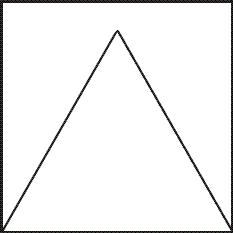
\includegraphics[width=0.25\textwidth]{\rootPath Imgs/qrcodes/joinup.png}%
\framedgraphics{width=0.25\textwidth}{\rootPath Imgs/qrcodes/octo/D.png}%
\includegraphics[width=0.25\textwidth]{\rootPath Imgs/qrcodes/joinup.png}%
\\%
\vspace{-2pt}\framedgraphics{width=0.25\textwidth}{\rootPath Imgs/qrcodes/octo/O.png}%
\hspace{-1pt}\framedgraphics{width=0.25\textwidth}{\rootPath Imgs/qrcodes/octo/C.png}%
\hspace{-1pt}\framedgraphics{width=0.25\textwidth}{\rootPath Imgs/qrcodes/octo/P.png}%
\\%
\vspace{-2pt}\includegraphics[width=0.25\textwidth]{\rootPath Imgs/qrcodes/joindown.png}%
\framedgraphics{width=0.25\textwidth}{\rootPath Imgs/qrcodes/octo/B.png}%
\includegraphics[width=0.25\textwidth]{\rootPath Imgs/qrcodes/joindown.png}\\

\vspace{0.5cm}
\caption{Patron de mire hémisphérique octogonale}\label{extra:patron_octo}
\end{figure*}

\end{document}

%----------------------------------------------------------------------

\clearpage
\phantomsection
\bibliographystyle{apalike}
\bibliography{\rootPath Annexes/biblio}

% \phantomsection \listoffigures

% \clearpage
% \begingroup
% 	\let\clearpage\relax
% 	\onecolumn
% 	\phantomsection \listoftables
% 	\phantomsection \listofalgorithms
% 	\phantomsection \listofcode
% \endgroup

%\addcontentsline{toc}{section}{Table des matières}
%\printindex

%======================================================================
\end{document}
%======================================================================
